\documentclass[paper=A4,DIV=calc]{scrartcl}
%\documentclass[draft,paper=A4]{scrartcl}

\newif\ifhtml
% HTML generation (.doc-conversion) > set html to true and use htlatex. else set html to false
%\htmltrue
%\htmlfalse

\ifhtml % In case of web format output...
	\def\pgfsysdriver{pgfsys-tex4ht.def}	
	\usepackage[dvips]{graphicx}
\else
   \usepackage{graphicx}
\fi

\usepackage[ansinew]{inputenc} 						% so I can write my Name without \"{u}
\usepackage[T1]{fontenc} 							% Standard Latex-Fonts
\usepackage[english]{babel}
\usepackage{svn-multi} 								% to add SVN-Versioning-Info
\usepackage{caption,subfig}                         % [font = small]
\usepackage[alsoload=binary]{siunitx}		 		% typographically correct units (\milli\meter, \kilo\electronvolt), with [alsoload=binary] \SI{100}{\giga\byte}
\usepackage{booktabs}		 						% nice tables
\usepackage{tikz} 									% extremely nice drawings
\usepackage{pgfplots} 								% ditto for plots
\usepackage{lipsum}									% for blind-text
\usepackage{fancyhdr}
\usepackage{tikz}									% TikZ is no drawing program
\usepackage[numbers,square,sort&compress]{natbib} 	% nice bibliography
%\usepackage{endfloat}				 				% floats at the end, use [nomarker] if "Figure x approx. here" is undesired
%	\renewcommand{\efloatseparator}{}
%\usepackage{flafter} 								% floats after their first instance
%\usepackage{microtype} 							% for nicer typography
	%\DisableLigatures{encoding=T1}
%\usepackage{setspace}
%	\doublespacing
%	\onehalfspacing
%	\singlespacing

\ifhtml
	\usepackage{url}
	\usepackage{index}
	\usepackage{color}
	\newindex{todo}{todo}{tnd}{Todo List} 
	\newcommand{\todo}[1]{\textcolor{red}{[To do: #1]}\index[todo]{#1}}
\else
	\usepackage{lineno}
		% line numbers
		\linenumbers
		%\pagewiselinenumbers
		\modulolinenumbers[2]
	\usepackage[backref]{hyperref}					% backref generates link from references back to text
	\usepackage[]{todonotes} 		 				% [disable]
%	\hypersetup{pdfauthor={David Haberth�r},%
%				pdftitle={WideFieldScanPaper},%
%				pdfsubject={Tomography},%
%				pdfkeywords={tomography, synchrotron, microscopy, field of view, enhancement, simulation},%
%%				pdfborder={0 0 0},% > no border around links, but...
%%				colorlinks=true % ... colored (true > no border, use "false" for final output)
%				}
\fi

%% Subversion Information
\svnidlong
{$HeadURL$}
{$LastChangedDate$}
{$LastChangedRevision$}
{$LastChangedBy$}

\pagestyle{fancy}

\newcommand{\imsize}{\linewidth}
\newlength\imagewidth % needed for scalebars
\newlength\imagescale % needed for scalebars

%from http://tinyurl.com/38rqn4 to use for institutions...
\newcommand{\footremember}[2]{\footnote{#2}\newcounter{#1}\setcounter{#1}{\value{footnote}}}
\newcommand{\footrecall}[1]{\footnotemark[\value{#1}]} 

\title{Wide Field Scan Paper}
\ifhtml % In case of web format output...
    \author{David Haberth�r \and Christoph Hinterm�ller \and Johannes Schittny \and Marco Stampanoni}
	\date{\today}
\else
    \author{David Haberth�r\footremember{ana}{Institute of Anatomy, University of Bern, Switzerland}%   
		\and Christoph Hinterm�ller\footremember{sls}{Swiss Light Source, Paul Scherrer Institut, Villigen, Switzerland}%
		\and Johannes Schittny\footrecall{ana} \footnote{corresponding author: \href{mailto:johannes.schittny@ana.unibe.ch}{johannes.schittny@ana.unibe.ch}}%
		\and Marco Stampanoni\footrecall{sls} \footnote{Institute of Biomedical Engineering, University and ETH Z�rich, Switzerland}}
    \date{Version of \svnfileday.\svnfilemonth.\svnfileyear \space \svnfilehour:\svnfileminute \space (UTC\svnfiletimezone), Revision \svnkw{LastChangedRevision}.} 
\fi

\begin{document}

\maketitle

\begin{abstract}
State-of-the-art synchrotron-based tomographic microscopy end-stations acquire volumetric data at micrometer level within a few minutes. It is therefore possible to investigate large objects at a high resolution by stacking several tomograms together and perform a local tomographic reconstruction.

The stacking of tomograms increases the field of view in vertical direction. The present work aims to implement the necessary acquisition protocols at the TOMCAT beamline of the Swiss Light Source to increase the field of view of the tomographic imaging process in horizontal direction. It is the base for imaging of samples bigger than the size currently possible. Different image acquisition protocols have been implemented for the end-user at the beamline. We have shown that the lateral field of view of TOMCAT can be increased up to five times and provide the end-user of the beamline the possibility to acquire quality guided tomographic wide field scans of his sample in an unattended, automatic way.
\end{abstract}

\begin{center}
	\fbox{
		\begin{minipage}{.618\textwidth}
		The file \url{\svnkw{HeadURL}}, was last changed at: \svnfileday.\svnfilemonth.\svnfileyear \space \svnfilehour:\svnfileminute \space (UTC\svnfiletimezone) and is at revision \svnkw{LastChangedRevision}.
		\end{minipage}
	} 
\end{center}

\ifhtml
	\emph{Did you sort out all todos?}
\else
	\listoftodos
\fi

%\tableofcontents

%!TEX root = widefieldscan.tex
\svnidlong
{$HeadURL$}
{$LastChangedDate$}
{$LastChangedRevision$}
{$LastChangedBy$}

\ifhtml
\else
\begin{center}
	\fbox{
		\begin{minipage}{.618\columnwidth}
		The section below is versioned at \url{\svnkw{HeadURL}} (last commit @ \svnfileday.\svnfilemonth.\svnfileyear \space \svnfilehour:\svnfileminute, Revision: \svnkw{LastChangedRevision}).
		\end{minipage}
	} 
\end{center}
\fi

\section{Introduction}%
Synchrotron radiation based x-ray tomographic microscopy (SRXTM) is a powerful method for the non-destructive three-dimensional imaging of a broad kind of materials with a resolution on the sub-micrometer scale.

At TOMCAT---the beamline for TOmographic Microscopy and Coherent rAdiology experimenTs~\cite{Stampanoni2007} at the Swiss Light Source (SLS), Paul Scherrer Institute, Villigen, Switzerland---many user groups are presently working in diverse research areas, ranging from biology~\cite{McDonald2009,PerezHuerta2009}, biomedical research~\cite{Schittny2008,Tsuda2008,Heinzer2008} and paleontology~\cite{Gostling2008,Friis2007,Hagadorn2006,Donoghue2006} to material science~\cite{Gallucci2007}, geology~\cite{Carminati2007} to process engineering~\cite{Davenport2007,Vaucher2007}.

We are studying the structural alterations of the lung parenchyma throughout development using SRXTM. In particular we are interested in the development of the acini over the course of the postnatal lung development in mammals. An acinus represents the functional respiratory lung unit containing groups of alveoli, where the gas-exchange in the lung takes place and is defined as the complex of alveolated airways distal to the terminal bronchiole~\cite{Rodriguez1987}.

Until now, the investigation of the three dimensional structure of an acinus was either limited by the resolution of the imaging method (in the case of micro-computed tomography (\micro CT)) or the sample volume (in the case of SRXTM).  The available field of view of microscopy based imaging methods like synchrotron based tomographic beam lines and lab-based \micro CT stations is limited by the camera and microscope optics. Commonly a larger field of view resulting in a larger sample volume is traded against a lower magnification. Therefore, at TOMCAT the sample volume is limited to a cylinder with a diameter of \SI{1.52}{\milli\meter} and a height of \SI{1.52}{\milli\meter}, if only one tomogram is taken at a resolution of \SI{1.48}{\micro\meter}.

Samples of a diameter larger than the FOV in the direction perpendicular to the rotational axis require local tomography. During local tomography only the central cylinder where every part of the sample is included on the projectional image of every rotational angle may be reconstructed without artifacts. These artifacts are introduced due to the fact that lateral regions of the sample not included in all projectional images of every rotational angle (i.e.\ partial volume effects). Generally, a local tomography approach is not suitable for studies investigating the development~\cite{Schittny2008,Mund2008} and structure~\cite{Tsuda2008} of lungs using SRXTM, which require high resolution datasets providing a large lateral field of view.

To overcome these limitation, we developed a synchrotron radiation x-ray tomographic microscopy method which combines several tomographic scans into one large three dimensional dataset increasing the scanned volume up to 25 times.

\subsection{Enhancing the Field of View}%
\label{subsec:enhancing the field of view}%
An increase of the field of view parallel to the rotation axis of the sample can be achieved through the stacking of multiple scans on top of each other. For this protocol, the scan time is linearly increasing with the number of scans required to cover the size of the sample. Due to the restrictions implied by the sampling theorem this approach can not directly be used to increase the field of view horizontal to the rotation axis. The sampling theorem states, that we need to acquire an amount of projections $P=D\frac{\pi}{2}$ for a detector width $D$.

As a consequence, when enlarging the field of view perpendicular to the rotation axis it is necessary to record more projections at the lateral parts of the sample compared to the central parts of the sample to equally fulfill the sampling theorem. This leads to an increase in acquisition and post-processing time as compared to a standard scan. We defined and validated multiple scanning protocols to decrease the acquisition time and performed three-dimensional reconstructions of datasets with increased lateral field of view of up to \SI{7}{\milli\meter} at a voxel size of \SI{1.48}{\micro\meter}.
%!TEX root = widefieldscan.tex
\svnidlong
{$HeadURL$}
{$LastChangedDate$}
{$LastChangedRevision$}
{$LastChangedBy$}

\begin{center}
	\fbox{
		\begin{minipage}{.618\textwidth}
		The file of this section is \url{\svnkw{HeadURL}}, was last changed at: \svnfileday.\svnfilemonth.\svnfileyear \space \svnfilehour:\svnfileminute \space (UTC\svnfiletimezone) and is at revision \svnkw{LastChangedRevision}.
		\end{minipage}
	} 
\end{center}

\section{Materials and Methods}
\label{sec:materials and methods}
\subsection{Animal Handling and Tissue Preparation}
The preparation of the lung samples has been performed according to~\citet{Schittny1997,Schittny1998}. Briefly, the lungs have been extracted from Sprague-Dawley rats after they have been perfused and filled with phosphate buffered saline by instillation via tracheostomy until the midrespiratory lung volume was reached.

The extracted lung lobes have been fixed for potential storage in 2.5\% glutaraldehyde (C$_5$H$_8$O$_2$). For the preparation of the imaging the samples have been postfixed---as in electron microscopy---with 1\% osmium tetroxide (OsO$_4$) and stained with 4\% uranyl acetate (C$_4$H$_6$O$_6$U), dehydrated in a graded series of ethanol and transferred into paraffin. \todo{Citation needed! Or longer explanation} Osmium tetroxide and uranyl acetate exhibit a higher absorption contrast for x-rays than the unstained lung tissue, thus facilitating the imaging of the stained tissue. The lung samples have been mounted onto standard electron microscopy sample mounts with a diameter of approximately \SI{13}{\milli\meter} (PLANO GmbH, Wetzlar, Germany) using paraffin.

Handling of the animals before and during the experiments, as well as the experiments themselves, were approved and supervised by the Swiss Agency for the Environment, Forests and Landscape and the Veterinary Service of the Canton of Bern.

\subsection{SRXTM}
The experiments were performed on the TOMCAT beamline at the Swiss Light Source, Paul Scherrer Institut, Villigen, Switzerland. TOMCAT is one of 15 currently operating beam lines at the SLS. TOMCAT is located at the port X02DA of the SLS. The beamline receives photons from a \SI{2.9}{\tesla} super-bending magnet. The critical energy of this super-bending magnet is \SI{11.1}{\kilo\electronvolt} (corresponding to a wavelength of \SI{0.122}{\nano\meter}). A double crystal multilayer monochromator covers an energy range between 6 and \SI{45}{\kilo\electronvolt} with a bandwidth of a few percent down to \SI{e-4}. Detailed technical specifications of the beamline and beam characteristics have been described by~\citeauthor{Stampanoni2006a}~\cite{Stampanoni2006a,Stampanoni2007}.

\subsubsection{Image Acquisition}
\label{seq:Image Acquisition}
The sample holder at TOMCAT is equipped with an appropriate collet chuck to mount standard electron microscopy (EM) sample tables into the beam. The samples have been scanned at an x-ray energy of \SI{12.6}{\kilo\electronvolt}. After penetration of the sample, the x-rays are converted into visible light by a Ce-doped YAG scintillator (Crismatec Saint-Gobain, Nemours, France). The projection images were further magnified by diffraction limited microscope optics and digitized by a high-resolution 2048$\times$2048 pixel CCD camera (PCO AG, Kelheim, Germany) with 14 bit nominal dynamic range which can record projections into the internal memory of \SI{4}{\giga B}. All samples were imaged using a 10$\times$ magnification, with 2$\times$2 binning and \SI{125}{\milli\second} exposure time or no binning and \SI{500}{\milli\second} exposure time, resulting in isotropic voxels with a side length of \SI{1.43}{\micro\meter} or \SI{0.72}{\micro\meter}, respectively.

\subsubsection{Generation of tomographic datasets}
The principles of x-ray computed tomography are explained in details by \citet{Kak2002} and \citet{Hsieh2003}. Briefly, projection images $I_{Pr}$---essentially single radiographies---of the sample are recorded at several angular positions between \SI{0}{\degree} and \SI{180}{\degree}. Additionally, a set of dark ($I_{D}$) and flat images ($I_{F}$) are recorded. The dark image set is obtained with a closed shutter at the start of the scan, it captures the camera noise and dark current and are used to baseline correct the projection images. The flat image set is recorded at the start and at the end of the scan, it captures the beam profile and are used to normalize the projection images. The corrected projection images $I_{cPr}$ are then computed corrected with the average dark ($\overline{I_{D}}$) and average flat image ($\overline{I_{F}}$) using equation~\ref{eq:cpr}.
\begin{equation}
	I_{cPr} = -ln\left(\frac{I_{Pr}-\overline{I_{D}}}{\overline{I_{F}}-\overline{I_{D}}}\right)=ln(\overline{I_{F}}-\overline{I_{D}})-ln(I_{Pr}-\overline{I_{D}})
\label{eq:cpr}
\end{equation}
The corrected projections are then transformed into so-called sinograms, where the $n$\textsuperscript{th} is composed of the $n$\textsuperscript{th} line of every corrected projection. One sinogram thus contains as many rows as the amount of obtained corrected projections---the angular steps---and as many columns as the width of the projection images. Each sinogram corresponds to one slice of the full tomographic dataset. The $n$\textsuperscript{th} slice of the resulting tomographic scan can be reconstructed from the $n$\textsuperscript{th} sinogram using for instance a standard filtered back-projection~\cite{Kak2002,Hsieh2003} or gridrec~\cite{Dowd1999} algorithm. The absorption properties of the sample are encoded by the gray values of the reconstructed dataset. The full work flow from image acquisition to tomographic dataset on the disk contains several steps more, all the details are explained by~\citet{Hintermueller2009}.

\subsection{Wide Field Scanning}
As mentioned in section~\ref{subsec:enhancing the field of view}, to obtain an enhanced FOV, we need to scan the samples with multiple subscans at varying positions covering the whole sample. To achieve this, we have written a custom MATLAB-script \todo{Script(s) in Appendix?}(MATLAB$^\text{\textregistered}$ 7.6.0.321 (R2008a), The MathWorks, Inc.), where the user is able to input the scanning parameters like desired FOV, detector width, desired overlap between the subscans, magnification and binning. The script then simulates different scanning protocols and calculates the expected reconstruction quality, which is then plotted against the acquisition time. Such a plot is shown in figure~\ref{fig:2008c-qualityplot}.

\begin{figure}
	\centering
		%\documentclass{article}
%\usepackage{tikz,pgfplots}
%\usepackage[pdftex,active,tightpage]{preview}
%\begin{document}
%\begin{preview}
\begin{tikzpicture}
\begin{axis}[%
	xlabel={estimated Scanning Time [min]},%
	ylabel={Expected Quality of the Scan [\%]},%
	]

% Line plot
\addplot [ color = red, only marks, mark = *] 
coordinates{
 (5.5875,10) (6.98958,51.0063) (8.3875,48.3324) (11.1813,69.4075) (11.6458,81.985) (13.975,80.0399) (16.3021,90.7093) (16.7688,85.096) (18.6354,93.3621) (19.5625,88.5423) (20.9625,96.7319) (22.3625,90.8617) (23.2917,96.3704) (25.1563,92.5481) (27.9479,98.2413) (27.95,93.8354) (30.2813,98.9979) (30.7437,94.8773) (31.4438,99.5581) (33.5375,95.6051) (34.9375,99.4314) (36.3375,96.2983) (39.1313,96.6062) (39.5938,99.5875) (39.5958,99.5241) (41.925,100) (41.925,96.9138) (41.9271,99.6929) (44.7188,97.1848) (46.5833,99.6309) (47.5125,97.3067) (50.3125,97.4836) (53.1063,97.603) (55.9,97.4336)
};

% Line plot
\addplot [ smooth ] 
coordinates{
 (5.5875,23.213) (6.98958,37.7379) (8.3875,50.0404) (11.1813,68.9695) (11.6458,71.4736) (13.975,81.6837) (16.3021,88.5733) (16.7688,89.6234) (18.6354,92.9028) (19.5625,94.0559) (20.9625,95.3079) (22.3625,96.078) (23.2917,96.3777) (25.1563,96.6032) (27.9479,96.3862) (27.95,96.3859) (30.2813,96.0569) (30.7437,96.0006) (31.4438,95.9286) (33.5375,95.8484) (34.9375,95.9383) (36.3375,96.1591) (39.1313,96.986) (39.5938,97.167) (39.5958,97.1679) (41.925,98.211) (41.925,98.211) (41.9271,98.212) (44.7188,99.5426) (46.5833,100.268) (47.5125,100.516) (50.3125,100.492) (53.1063,98.6574) (55.9,94.0299)
};


\pgfplotsset{every axis legend/.append style={
at={(0.618,0.2)},
anchor=base}}

\legend{Protocols,Polynomial Fit (x=4)}%$p(x)=p_{1}x^{n}+p_{2}x^{n-1}+...+p_{n}x+p_{n+1}$}

\end{axis}
\end{tikzpicture}
%\end{preview}
%\end{document}
	\caption{Quality-Plot of 34 calculated protocols. The red dots show the expected the quality of the, the black plot is a polynomial fit $p(x)$ with $n=4$ for $p(x)=p_{1}x^{n}+p_{2}x^{n-1}+...+p_{n}x+p_{n+1}$. 19 of these protocols have been scanned. Details of these scans are shown in table~\ref{tab:projections} and are discussed in section~\ref{sec: Results I}.}
	\label{fig:2008c-qualityplot}
\end{figure}

The proposed protocols are designed in such a way that the total scanning time---which scales with the total amount of recorded projections---can be greatly reduced. Depending on the demand of the end-user, we were able to reduce the total acquisition time by 86\percent, as can be seen in table~\ref{tab:projections}. Albeit this reduction introduces some artifacts in the dataset, an automated segmentation of the airways is still possible, as is shown later on.

\begin{table}
\centering
	\caption{Specification of different protocols and time used compared to gold standard}
	\begin{tabular*}{\textwidth}{l@{\extracolsep\fill}ccccccccccccccccccc}
		\toprule
		Protocol 			& B & C & D & E & F & G & H\\
		\midrule
		Total Projections 	& 15732 & 13110 & 13110 & 10925 & 11799 & 9833 & 10488\\
		Time [\%] 			& 100 & 83.33 & 83.33 & 69.44 & 75 & 62.5 & 66.67\\
%		\bottomrule
	\end{tabular*}
	\begin{tabular*}{\textwidth}{l@{\extracolsep\fill}ccccccccccccccccccc}
		\toprule
		Protocol 			& I & J & K & L & M & N \\
		\midrule
		Total Projections 	& 5436 & 8740 & 9177 & 7648 & 7866 & 6555 \\
		Time [\%] 			& 34.7 & 55.6 & 58.3 & 48.6 & 50 & 41.7 \\
%		\bottomrule
	\end{tabular*}
	\begin{tabular*}{\textwidth}{l@{\extracolsep\fill}ccccccccccccccccccc}
		\toprule
		Protocol 			& O & P & Q & R & S & T \\
		\midrule
		Total Projections 	& 6555 & 5244 & 4370 & 3933 & 2622 & 2185 \\
		Time [\%] 			& 41.7 & 33.3 & 27.8 & 25 & 16.7 & 13.9 \\
		\bottomrule
	\end{tabular*}
	\label{tab:projections}
\end{table}

After the user has chosen a suitable protocol, the MATLAB-script writes a preference file to the disk. This preference file is parsed by a custom Python-script to interact with the EPIC-System (Experimental Physics and Industrial Control System, \url{http://www.aps.anl.gov/epics/}), which is used to acces and control all hardware of the TOMCAT beamline. We thus perform several subscans without user intervention, execpt entry of the sample name. All parameters like filename-suffixes of the subscans, sample-position in relation to the beam, rotation angles and amount of projections to obtain for the subscans have been set beforehand by the MATLAB-script, also permitting a multiple batch scans of the same sample without any manual intervention. The sample on the sample holder was thus not touched during the acquisition of the 57 different subscans for the 19 protocols discussed lateron. 

\subsection{Image Processing}
\label{subsec:image processing}
After the acquisition of the sub-scan projection images, these image sets are corrected with the so called dark field and flat field images. The dark field images are obtained while all the shutters are closed---thus no x-rays are present---and are used for the detection of camera noise and dark current. The flat field images (FI) are obtained with x-ray beam, but without the sample. They are recorded to remove the varying beam profile brightness from the projection images. The projections (PI) are first baseline corrected, then the average of the dark images is subtracted and afterwards they are normalized into corrected projections (CPR) as seen in equation~\ref{eq:correction}:%
\begin{equation}
	\text{CPR}=-ln\left(\frac{\text{PI}}{\text{FI}}\right)=ln(\text{FI})-ln(\text{PI})
	\label{eq:correction}
\end{equation}

\subsubsection{Covering a broad FOV}
\label{subsec:covering a broad fov}
Generally, tomographic images are obtained in such a manner, that the sample is rotated for \SI{180}{\degree} while multiple projection images are obtained, as is shown in figure~\ref{fig:covering-one scan}. After reconstructing the sample, the images show the FOV of the camera.

\begin{figure}[tb]
	\centering
	\subfloat[\SI{180}{\degree}]{%\documentclass{article}
%\usepackage{tikz}
%\begin{document}

\begin{figure}[tb]
	\centering
	\begin{tikzpicture}
		%drawing grid
		%\draw[color=gray] (0,0) grid (8,1);
		%camera
		\draw (-.2,-.2) rectangle (1.2,1.2);
		\draw (.5,-.25) node [below] {camera};
		% beam
		\draw[<-] (1.2,0) -- (8,0);
		\draw[<-] (1.2,1) -- (8,1);
		\draw (2.5,1.25) node [above] {beam};
		\draw (6.5,1.25) node [above] {beam};
		%sample
		\draw (4.5,0.5) circle (.5);
		\draw (4.5,-.25) node [below] {sample};
		%sample rotation
		\draw[->] (4.5,0.25) arc (-90:90:.25);
	\end{tikzpicture}
	\caption{Covering the FOV -- one scan}
	\label{fig:covering-one scan}
\end{figure}

%\end{document}\label{subfig:cover180}}\\
	\subfloat[\SI{360}{\degree}]{%\documentclass{article}
%\usepackage[pdftex,active,tightpage]{preview}
%\usepackage{tikz}
%\usepackage{pgfplots}
%\usetikzlibrary{plotmarks}
%\begin{document}
%\begin{preview}
	\begin{tikzpicture}
		%drawing grid
		%\draw[color=gray] (0,0) grid (8,1);
		%camera
		\draw[fill=gray] (-.2,-.2) rectangle (1.2,1.2);
		\draw (.5,-.25) node [below] {camera};
		% beam
		\foreach \x in {0,...,10}
			\draw[gray!50,<-] (1.2,0.1*\x) -- (8,0.1*\x);
		\draw[<-] (1.2,0) -- (8,0);
		\draw[<-] (1.2,1) -- (8,1);			
		\draw (2.5,1.25) node [above] {beam};
		\draw (6.5,1.25) node [above] {beam};
		%sample
		\draw[ultra thick] (4.5,1) circle (1);
		\draw (4.5,-.25) node [below] {sample};
		%sample rotation
		\draw[thick,->] (4.5,0.75) arc (-85:265:.25);
	\end{tikzpicture}
%\end{preview}
%\end{document}\label{subfig:cover360}}
	\caption{Covering the FOV -- one scan}
	\label{fig:covering-one scan}
\end{figure}

\begin{figure}[tb]
	\centering
		\documentclass{article}
\usepackage[pdftex,active,tightpage]{preview}
\usepackage{tikz}
\usetikzlibrary{arrows,shapes,backgrounds}
\begin{document}
\begin{preview}
\begin{tikzpicture}%[ultra thick,scale=1]%,show background grid]
	%draw axes
		%\draw[ultra thick] (-10,0) -- (10,0);
		%\draw[ultra thick] (0,-10) -- (0,10);
		%\draw[ultra thick] (0,0) circle (.125);
	% rotation axis
		\draw[->] (0,-2) ++ (-50:.75) arc (-50:300:.75 and .25);
		\draw (0,-3) node [below] {Rotation axis} -- ++(0,2);
		\draw[dotted] (0,-1) -- ++(0,2);
		\draw (0,1) -- ++(0,0.25);
		\draw[dotted] (0,1.25) -- ++(0,2);
	% position 1
		\draw (0,-1) circle (1.5 and .5);
		\fill[shade,semitransparent] (-1.5,-1) arc (-180:0:1.5 and .5) -- ++(0,2) arc (0:180:1.5 and .5) -- cycle;
		\draw (-1.5,-1) arc (-180:0:1.5 and .5) -- ++(0,2) arc (0:180:1.5 and .5) -- cycle;		
		\draw (-1.5,1) arc (-180:0:1.5 and .5);
		\draw (1.5,0) node [right] {First Position};
	% position 2
		\draw (0,1.25) circle (1.5 and .5);
		\fill[shade,semitransparent] (-1.5,1.25) arc (-180:0:1.5 and .5) -- ++(0,2) arc (0:180:1.5 and .5) -- cycle;
		\draw (-1.5,1.25) arc (-180:0:1.5 and .5) -- ++(0,2) arc (0:180:1.5 and .5) -- cycle;		
		\draw (-1.5,3.25) arc (-180:0:1.5 and .5);
		\draw (1.5,2.25) node [right] {Second Position};
	% rotation axis on top
		\draw (0,3.25) -- ++(0,1.5);									
	% sample movement
		\draw[double,->] (-2.5,0) -- (-2.5,2.25) ;% node [text width=10cm,midway,left] {Sample movement relative to beam and camera};	
		% sample movement
		\node (movefrom) at (0,5.75) {Sample movement relative to beam and camera};
		\node (moveto) at (-2.5,1.125) {};
		\draw [->,dotted] (movefrom) to [bend right=54] (moveto);
\end{tikzpicture}
\end{preview}
\end{document}
	\caption{Stacked Scanning - long and thin samples}
	\label{fig:stacked-scanning}
\end{figure}

\begin{figure}[tb]
	\centering
		%\documentclass{article}
%\usepackage[pdftex,active,tightpage]{preview}
%\usepackage{tikz}
%\begin{document}
%\begin{preview}
\begin{tikzpicture}%[ultra thick,scale=1]%,show background grid]
	%draw axes
		%\draw[ultra thick] (-10,0) -- (10,0);
		%\draw[ultra thick] (0,-10) -- (0,10);
		%\draw[ultra thick] (0,0) circle (.125);
	% rotation axis
		\draw[->] (0,-3) ++ (-50:.75) arc (-50:300:.75 and .25);
		\draw[] (0,-4) node [below] {Rotation axis} -- ++(0,3);
		\draw[dotted] (0,-1) -- ++(0,2);
	% position 1
		\draw (0,-1) circle (1.5 and .5);
		\fill[shade,semitransparent] (-1.5,-1) arc (-180:0:1.5 and .5) -- ++(0,2) arc (0:180:1.5 and .5) -- cycle;
		\draw (-1.5,-1) arc (-180:0:1.5 and .5) -- ++(0,2) arc (0:180:1.5 and .5) -- cycle;		
		\draw (-1.5,1) arc (-180:0:1.5 and .5);
		\draw (1.25,-1.5) node [right] {First Position};
	% position 2
		\draw (0,-1) circle (4.5 and 1.5);
		\fill[shade,semitransparent] (-4.5,-1) arc (-180:0:4.5 and 1.5) -- ++(0,2) arc (0:180:4.5 and 1.5) -- cycle;
		\draw (-4.5,-1) arc (-180:0:4.5 and 1.5) -- ++(0,2) arc (0:180:4.5 and 1.5) -- cycle;		
		\draw (-4.5,1) arc (-180:0:4.5 and 1.5);
		\draw (2.25,-2.7) node [right] {Second Position};
	% top from position 1 on top
		\draw (0,1) circle (1.5 and .5);
	% rotation axis on top
		\draw (0,1) -- ++(0,2.5);									
	% sample movement
		\draw[double,->] (0,1) -- (3,1);
		\node (movefrom) at (0,4.5) {Sample movement relative to beam and camera};
		\node (moveto) at (2,1) {};
		\draw [->,dotted] (movefrom) to [bend left=45] (moveto);
\end{tikzpicture}
%\end{preview}
%\end{document}
	\caption{Stacked Scanning - broad samples}
	\label{fig:widefield-scanning}
\end{figure}

If we want to achieve tomographic scans covering a broader FOV, we have to move the sample in relation to the beam and camera, to be able to record projection images from the lateral parts of the sample. This can be done as shown in figure~\ref{fig:covering-three scans a}, \todo{which image variant: \ref{fig:covering-three scans a} or \ref{fig:covering-three scans b}?} where we obtain three subscans to be able to reconstruct a FOV covering the whole sample.

\begin{figure}[tb]
	\centering
	%\documentclass{article}
%\usepackage[pdftex,active,tightpage]{preview}
%\usepackage{tikz}
%\usepackage{pgfplots}
%\usetikzlibrary{plotmarks}
%\begin{document}
%\begin{preview}
	\begin{tikzpicture}[scale=1]
		%drawing grid
%		\draw[color=gray] (0,0) grid (10,1);
		%camera
			\draw (-.1,-.1) rectangle (1.1,1.1);
			\draw (.5,-.35) node {camera};
		% sample positions
			\foreach \x in {1,2,3}{
				\draw     (3*\x,\x-1.5) circle (.5) circle (1.5);			
				\draw[->] (3*\x,\x-1.75) arc (-90:90:.25);
				\draw     (3*\x,-3.25+\x)node {Position \x};
				}
		% movement		
			\foreach \x in {1,2}{				
			    \draw[->]  (3*\x,0.25+\x) -- (3*\x,1+\x);
		% beam
				\draw[<-] (1.2,\x-1) -- (12,\x-1);
				}
	\end{tikzpicture}
%\end{preview}
%\end{document}
	\caption{Covering the FOV -- three scans $\rightarrow$ sample has to move, explain that we still only do \SI{180}{\degree} scans!}
	\label{fig:covering-three scans a}
\end{figure}

\begin{figure}[tb]
	\centering
	\documentclass{article}
\usepackage[pdftex,active,tightpage]{preview}
\usepackage{tikz}
\usepackage{pgfplots}
\usetikzlibrary{plotmarks}
\begin{document}
\begin{preview}
%%%%%%%%%%%%%%%%%%%%%%%%%%%%%%%%%
	\begin{tikzpicture}
		%camera
			\draw (-.1,-.1) rectangle (1.1,1.1);
			\draw (.5,-.35) node {camera};
		% sample positions
			\foreach \x/\color in {1/red,2/green,3/blue}{
				\draw[color=\color]    (5,\x-1.5) circle (.5) circle (1.5);			
				\draw[color=\color,->] (5,\x-1.75) arc (-90:90:.25);
				\draw[color=\color]    (7.5,\x-1.5) node {Position \x};
				}
		% movement		
			\foreach \x/\e/\color in {1/3.25/red,2/3.25/green}{				
			    \draw[color=\color,->] (\e,-1.5+\x) node [left] {mov. \x} -- (\e,-.5+\x);
			    }
			 \foreach \x in {1,2}{				
		% beam
				\draw[<-] (1.2,\x-1) -- (9,\x-1);
				}
	\end{tikzpicture}
%%%%%%%%%%%%%%%%%%%%%%%%%%%%%%%%%
\end{preview}	
\end{document}
	\caption{Or is this better for the understanding?: Covering the FOV -- three scans $\rightarrow$ sample has to move, explain that we still only do \SI{180}{\degree} scans!}
	\label{fig:covering-three scans b}
\end{figure}

To cover the desired FOV, the projection images have to be obtained in such a manner that they overlap each other slightly. This overlap is necessary for the compensation of variations in the imaging process and correct stitching of the single projections into one big projection image. 

After correction, the projections of the single overlapping subscans are merged into one projection which covers the full FOV chosen by the user (see figure~\ref{fig:merge-proj}). To achieve a correct stitching of the multiple sub-scan projections into one projection coverint the full FOV, the cutting line between adjacent subscans has to be calculated. According to~\citet{Hintermueller2009} the cutting line to remove the overlap is calculated using the mean squared difference between adjacent subscan images. Briefly, for each displacement $\xi_{i,j}$ of the images $i$ and $j$ the mean squared difference of the displacement $\delta^2(\xi_{i,j})$ is computed. This directly provides a measure for the inequality of the two images within their overlapping parts. The local minimum of $\delta^2(\xi_{i,j})$ shows the effective displacement $\xi_{i,j}$ between the two adjacent images $i$and $j$. For three subscans we calculate the effective displacement $\xi_{1,2}$ and $\xi_{2,3}$ and stitch all the images into one big projection image.

Since the amount of obtained projection varies for different positions of the sample in relation to the camera window---at outer positions we record more projections compared to central positions to fulfill the sampling theorem---different amounts of projections have been obtained for each subscan. If $N_x$ is the total amount of projections for each subscan we cannot simply stitch together all the images from 1 to $N$ for each subscan $x$, or we will end up with wrong merged projections. Instead, we have to stitch them together in such a way that we chose the correspondent adjacent projections. \todo{Mention potential interpolation of the inner scans?}

All above mentioned steps have been implemented in a custom MATLAB\textsuperscript{\textregistered} function which takes the parameters of the single subscans (e.g.\ Samplename, Amount of subscans, Amount of Dark and Flat images) and desired Output-Name and -Suffix as inputs and performs all necessary calculations like loading, normalizing, interpolation and correct stitching of the images into wide field projections. Excemplary results can be seen in figure~\ref{fig:wide field scan results}\subref{fig:subscans} and \ref{fig:wide field scan results}\subref{fig:merge-proj}.

After the merging of the normalized projections, the merged projections were reconstructed into the virtual tomography slices using a standard filtered backprojection algorithm or a FFT-based gridrec algorithm~\cite{Dowd1999} on a 20-node server farm (Pentium 4, 2.8 GHz processor, 512 MB RAM \todo{cluster node specs?}). This reconstruction results in an image stack of 1024 or 2048 image slices in tif-format, depending on the binnig chosen at recording time. The size of the images recorded for this publication varies from 2996$\times$2996 pixels up to 9703$\times$9703 pixels.
%!TEX root = widefieldscan.tex
\svnidlong
{$HeadURL$}
{$LastChangedDate$}
{$LastChangedRevision$}
{$LastChangedBy$}

\ifhtml
\else
\begin{center}
	\fbox{
		\begin{minipage}{.618\columnwidth}
		The section below is versioned at \url{\svnkw{HeadURL}} (last commit @ \svnfileday.\svnfilemonth.\svnfileyear \space \svnfilehour:\svnfileminute, Revision: \svnkw{LastChangedRevision}).
		\end{minipage}
	} 
\end{center}
\fi

\section{Results}%
\label{sec:Results}%
\subsection{Image Merging and Reconstruction}%
\label{sec:Image Merging and Reconstruction}%
Multiple independently acquired projection images covering the desired FOV have been merged into single projections covering the full FOV. Figure~\ref{fig:subscans} shows exemplary projection images from overlapping subscans prior to correction and normalization. Figure~\ref{fig:merge-proj} shows a merged projection image prior to reconstruction and figure~\ref{fig:merge-rec} shows one slice of the reconstructed dataset acquired from 5244 projections. Such a reconstructed slice covers a FOV of \SI{2792}{pixels} (\SI{4.13}{\milli\meter}) which is three times the size of what can be achieved with one single binned scan (\SI{1024}{pixels} or \SI{1.52}{\milli\meter}). %1024 * 1.48 um/px = 1.51552mm

%%% iucr %%%
%\onecolumn
\begin{figure}%
	\caption{Wide field scan of a rat lung sample obtained from a Sprague-Dawley rat 21 days after birth, showing the distal-medial edge of the right lower lung lobe. The sample has been scanned at \SI{12.6}{\kilo\electronvolt}, the protocol details conform to protocol ``B'', described in table~\ref{tab:protocols}.}%
	\label{fig:wide field scan results}%
	\begin{tabular}{p{.75\linewidth}}%
	%\documentclass{article}
%\usepackage{subfig}
%\usepackage{tikz}
%\usepackage{siunitx}
%\begin{document}
%\newcommand{\imsize}{\linewidth}
%\newlength\imagewidth % needed for scalebars
%\newlength\imagescale % needed for scalebars
%\begin{figure}
%	\centering
%%%%%%%%%%%%%%%%%%%%%%%%%%%%%
	\renewcommand{\imsize}{.333\linewidth}
	\pgfmathsetlength{\imagewidth}{\imsize} % desired display width of image
	\pgfmathsetlength{\imagescale}{\imagewidth/1024} % pixel width of image
			% --------------------------------------------------------------
			% Cutline between SubScan 1 and 2: 141 pixels
			% Cutline between SubScan 2 and 3: 138 pixels
			% --------------------------------------------------------------
			\def\size{1023}%
			\begin{tikzpicture}[x=\imagescale,y=-\imagescale]%
				\node[anchor=north west, inner sep=0pt, outer sep=0pt] at (0,0)%
					{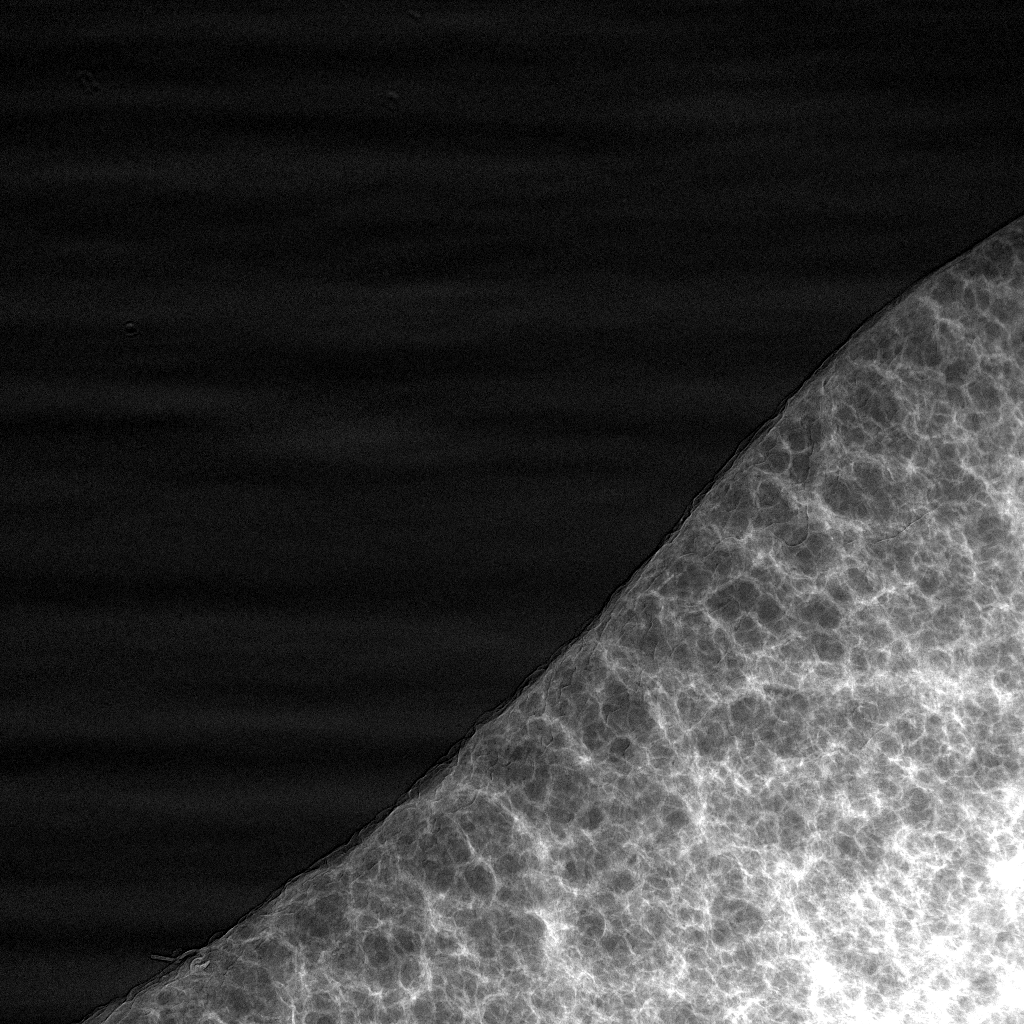
\includegraphics[width=\imagewidth]{img/merge/CP-R108C21Cb_s13358_normalize}};%
%					{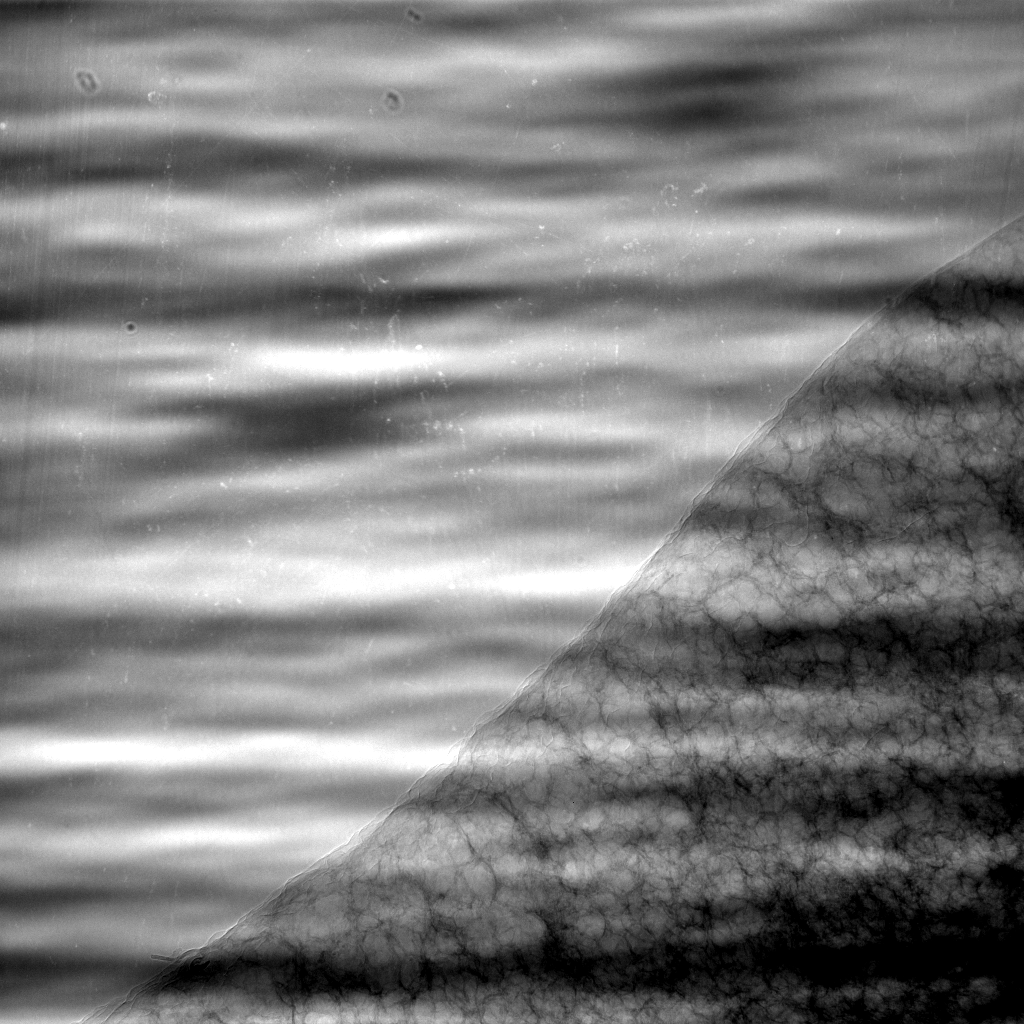
\includegraphics[width=\imagewidth]{R108C21Cb_s13358_normalize}};%
				\def\overlap{141}%
				\fill [red, nearly transparent] (1024-\overlap,1) rectangle (\size,\size);%
				\draw (1024-\overlap,1) rectangle (\size,\size);%
				\node [anchor=south west, color=white] at (0,1024) {(a)};				
			\end{tikzpicture}%
			\begin{tikzpicture}[x=\imagescale,y=-\imagescale]%
				\node[anchor=north west, inner sep=0pt, outer sep=0pt] at (0,0)%
					{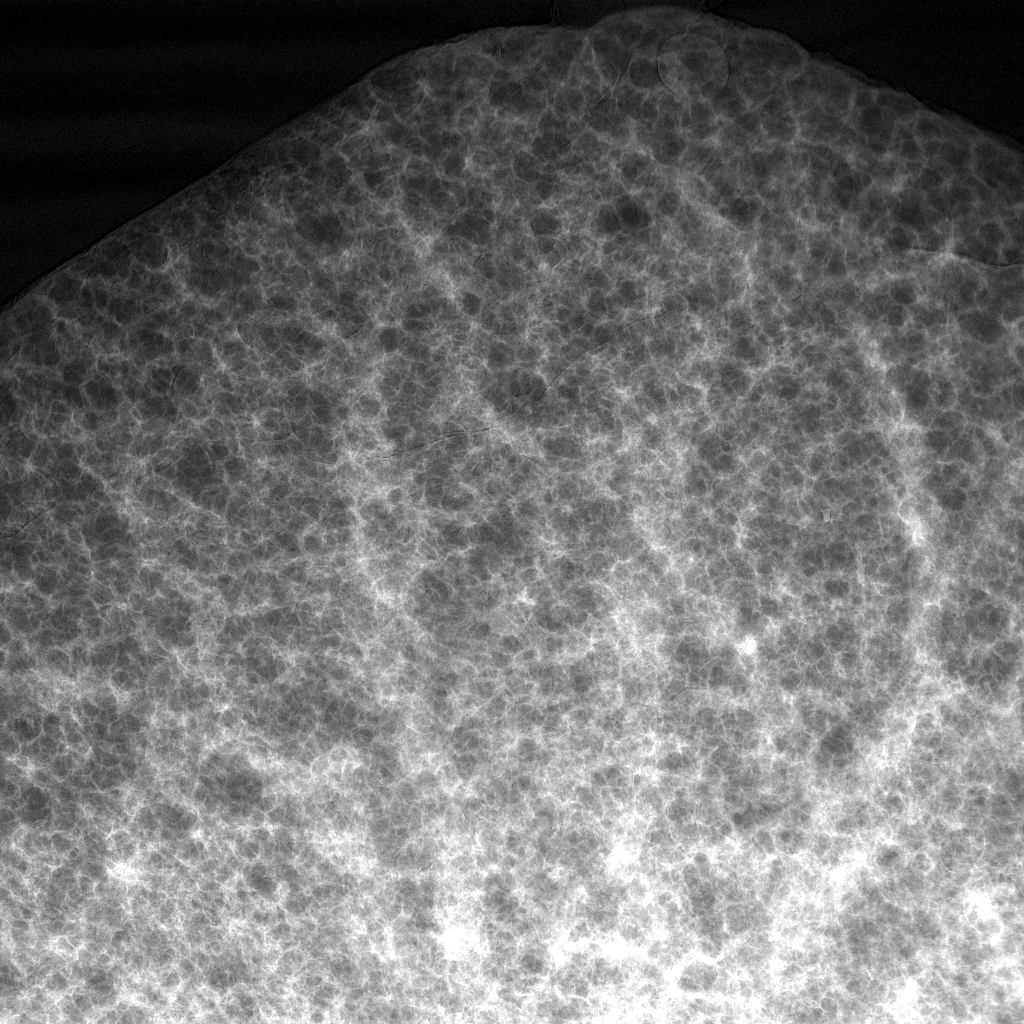
\includegraphics[width=\imagewidth]{img/merge/CP-R108C21Cb_s23358_normalize}};%
%					{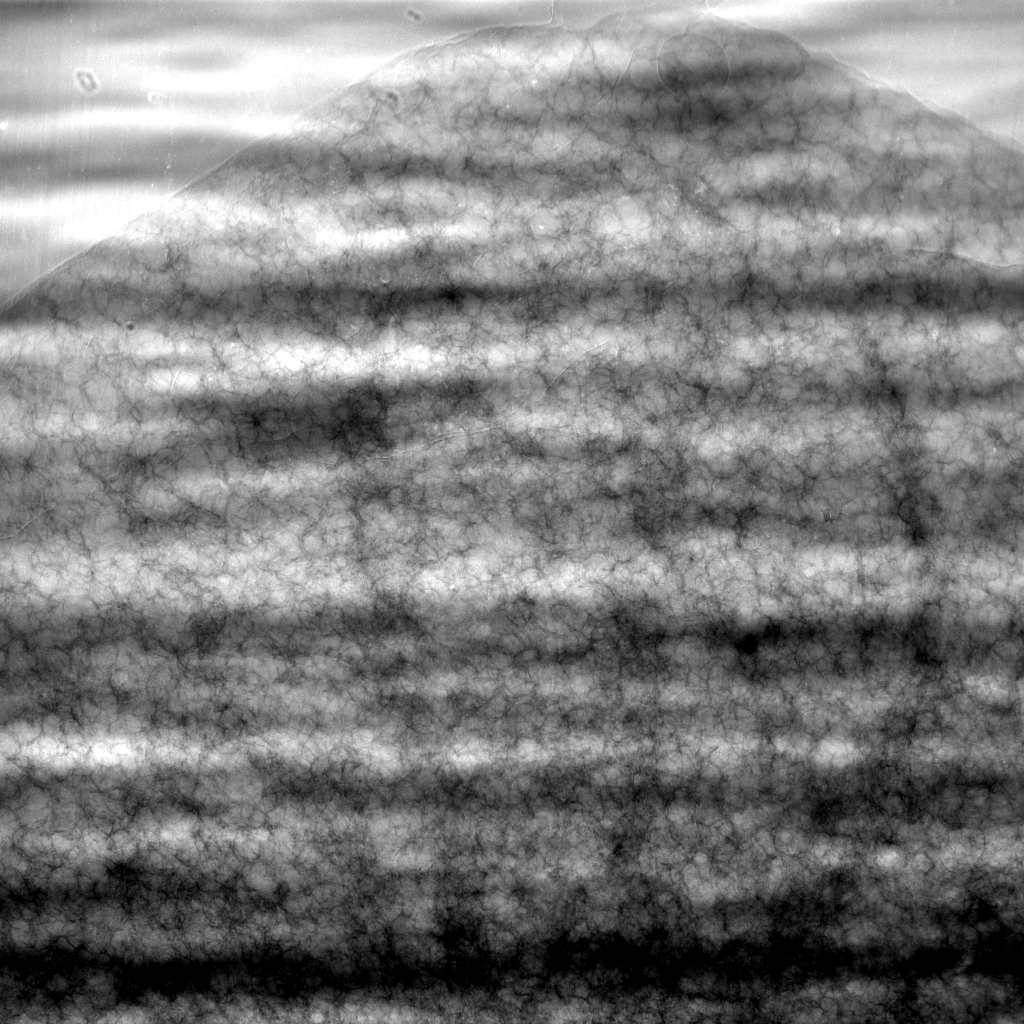
\includegraphics[width=\imagewidth]{R108C21Cb_s23358_normalize}};%
				\def\overlap{141}%
				\fill [green, nearly transparent] (1,1) rectangle (\overlap,\size);%
				\draw (1,1) rectangle (\overlap,\size);%
				\def\overlap{138}%
				\fill [blue, nearly transparent] (1024-\overlap,1) rectangle (\size,\size);%
				\draw (1024-\overlap,1) rectangle (\size,\size);%
			\end{tikzpicture}%
			\begin{tikzpicture}[x=\imagescale,y=-\imagescale]%
				% place image (integer coordinates refer to pixel centers):
				\node[anchor=north west, inner sep=0pt, outer sep=0pt] at (0,0)%
					{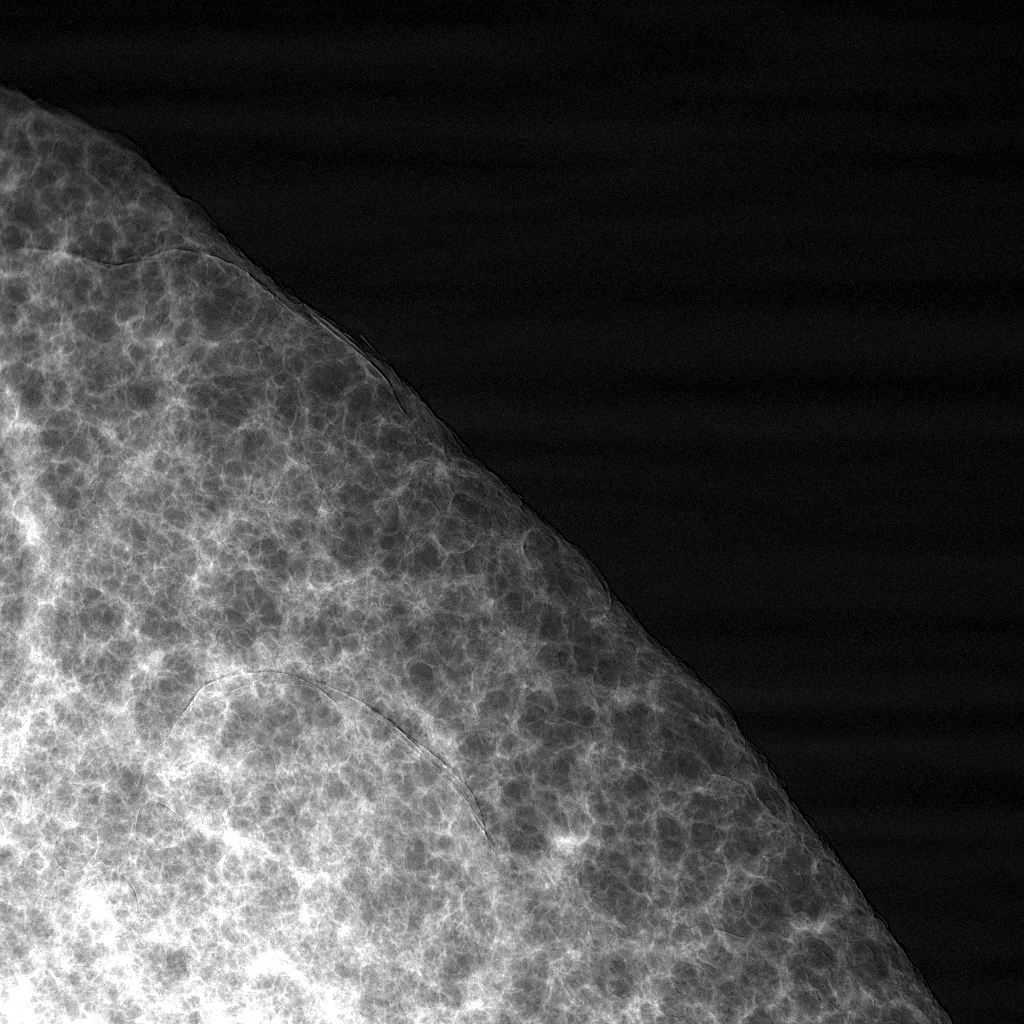
\includegraphics[width=\imagewidth]{img/merge/CP-R108C21Cb_s33358_normalize}};%
%					{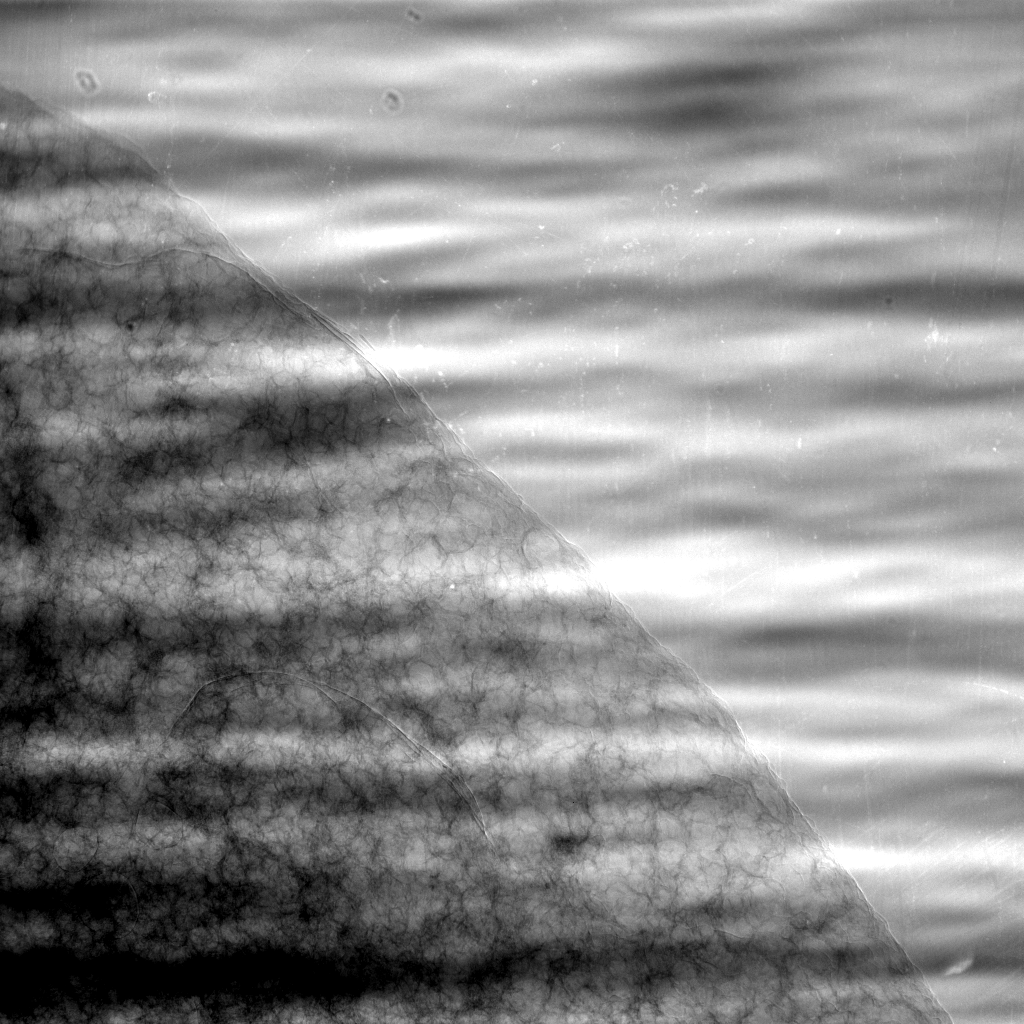
\includegraphics[width=\imagewidth]{R108C21Cb_s33358_normalize}};%
				\def\overlap{138}%
				\fill [yellow, nearly transparent] (1,1) rectangle (\overlap,\size);%
				\draw (1,1) rectangle (\overlap,\size);%
%				\draw[|-|,thick] (5,200) -- (1021,200) node [color=white,midway,above] {\SI{1.51552}{\milli\meter}};%
				\def\x{924}% 1024 - 100
				\def\y{922}% 1024 * .9 = 921.6
				\def\bar{338}% 100 px = 148 um
				\draw[|-|,thick, color=white] (\x-\bar,\y) -- (\x,\y) node [midway, above] {\SI{500}{\micro\meter}};%
			\end{tikzpicture}%
			\label{fig:subscans}%
%%%%%%%%%%%%%%%%%%%%%%%%%%%%%	
%	\caption{caption}
%\end{figure}
%\end{document}\\%
	a) Three uncorrected and independent projection images from subscans s$_1$--s$_3$, each with a size of 1024\(\times\)1024 pixels at a resolution of \SI{1.48}{\micro\meter\per pixel}, each covering a FOV of \SI{1.52}{\milli\meter}. Subscans s$_1$ and s$_2$ overlap each other by 141 pixels (red and green overlay), subscans s$_2$ and s$_3$ overlap each other by 138 pixels (blue and yellow overlay). 5244 projections  over a rotation of \SI{180}{\degree} have been acquired for all subscans.%
	\\%
	%\documentclass{article}
%\usepackage{subfig}
%\usepackage{tikz}
%\usepackage{siunitx}
%\begin{document}
%\newcommand{\imsize}{\linewidth}
%\newlength\imagewidth % needed for scalebars
%\newlength\imagescale % needed for scalebars
%\begin{figure}
%	\centering
%%%%%%%%%%%%%%%%%%%%%%%%%%%%%
		\renewcommand{\imsize}{\linewidth}%
		\pgfmathsetlength{\imagewidth}{\imsize} % desired displayed width of image
		\pgfmathsetlength{\imagescale}{\imagewidth/2793}% pixel width of image
			\begin{tikzpicture}[x=\imagescale,y=-\imagescale]%
				\node[anchor=north west,inner sep=0pt,outer sep=0pt] at (0,0)%
					{\includegraphics[width=\imagewidth]{img/merge/R108C21Cb_mrg3333_normalize}};%
%					{\includegraphics[width=\imagewidth]{R108C21Cb_mrg3333_normalize}};%
				\def\x{2693} % 2793-100
				\def\y{922} % 1024*.9 = 921.6
				\def\bar{338} % 100 px = 148 um
				\draw[|-|,thick,color=white] (5,256) -- (2787,256) node [midway,above] {\SI{4.13364}{\milli\meter}};
				\draw[|-|,thick,color=white] (\x-\bar,\y) -- (\x,\y) node [midway,above] {\SI{500}{\micro\meter}};
				\node [anchor=center,color=white] at (100,1024-100) {b)};
				\end{tikzpicture}%
			\label{fig:merge-proj}%
%%%%%%%%%%%%%%%%%%%%%%%%%%%%%	
%	\caption{caption}
%\end{figure}
%\end{document}\\%
	b) Merged and corrected image from the three subscans shown in subfigure a). Each merged projection has a size of 2793\(\times\)1024 pixels at a resolution of \SI{1.48}{\micro\meter\per pixel}. The width of the merged projections is slightly smaller than three times the width of the subscans due to the overlap needed to merge the projections (2793~px$=3\cdot3072$~px$-141$~px$-138$~px). Since the x-ray beam is extremely stable, the bands visible in the raw projections can be eliminated.%
	\\%
	%\documentclass{article}
%\usepackage{subfig}
%\usepackage{tikz}
%\usepackage{siunitx}
%\begin{document}
%\newcommand{\imsize}{\linewidth}
%\newlength\imagewidth % needed for scalebars
%\newlength\imagescale % needed for scalebars
%\begin{figure}
%	\centering
%%%%%%%%%%%%%%%%%%%%%%%%%%%%%
		\pgfmathsetlength{\imagewidth}{\imsize}%
		\pgfmathsetlength{\imagescale}{\imagewidth/2792}%
			\begin{tikzpicture}[x=\imagescale,y=-\imagescale]%
				\node [anchor=north west,inner sep=0pt,outer sep=0pt] at (0,0)%
					{\includegraphics[width=\imagewidth]{img/merge/R108C21Cb_mrg1024rec8bit}};% ``mogrify -shave 0x900 -format png R108C21Cb_mrg1024rec8bit.tif''
%					{\includegraphics[width=\imagewidth]{R108C21Cb_mrg1024rec8bit}};
				\clip (0,0) rectangle (2792,992);				
				\def\x{2692} % 2792-100
				\def\y{893} % 992 * .9 = 892.8
				\def\bar{338} % 100 px = 148 um
				%%%% scalebar
					\draw[|-|,thick,color=white] (\x-\bar,\y) -- (\x,\y) node [midway, above] {\SI{500}{\micro\meter}};
%					\draw[|-|,thick,color=white] (5,30) -- (2787,30) node [midway, below] {\SI{4.13216}{\milli\meter}};
				%%%% center
					\fill [color=red] (2792/2,992/2) circle (5);
				%%%% big circle
					\draw [dashed, ultra thick, color=red] (2792/2,992/2) circle (512);
					\def\angle{35}
					\draw [white, thick, <->] (2792/2,992/2) +(\angle:0) --  node (bigto) {} +(\angle:512); 
					\node [white] (bigfrom) at (349,256){$\frac{1024}{2}$px};
					\draw [white, ->, thick, densely dotted] (bigfrom) to [bend left=45] (bigto);
				%%%% big circle
				%%%% 141px circle
				\draw [dashed, ultra thick, color=red] (2792/2,992/2) circle (512-141);
				\def\angle{35+90}
					\draw [white,thick,<->] (2792/2,992/2) +(\angle:0) -- node (smallto) {} +(\angle:512-141);
					\node [white] (smallfrom) at (349,384) {$\frac{1024}{2}-141$px};
					\draw [white, ->, thick, densely dotted] (smallfrom) to [bend left=45] (smallto);
				%%%% 141px circle					
%				%%%% 138px circle
%				\draw [dashed,color=red] (2792/2,992/2) circle (512-138);
%				\def\angle{45+90+90}
%					\draw [white,<->] (2792/2,992/2) +(\angle:0) -- node (vsmallto) {} +(\angle:512-138);
%					\node [white] (vsmallfrom) at (2972-768,992-512) {$\frac{1024}{2}-138$px};
%					\draw [white,->,densely dotted] (vsmallfrom) to [bend right=45] (vsmallto);
%				%%%% 138px circle
				%%%% inset
%				\newcommand{\size}{.2\imagewidth}%
%				\clip (256,256) rectangle (512,512);
%				\node[anchor=north west,inner sep=0pt,outer sep=0pt] at (0,0)
%					{\includegraphics[width=\size]{R108C21Cb_mrg1024rec8bit}};
%					\draw[white] (0,0) rectangle (\size,-\size);
				%%%% inset
				\node [anchor=south west, color=white] at (0,990) {(c)};			
				\end{tikzpicture}%
			\label{fig:merge-rec}%
%%%%%%%%%%%%%%%%%%%%%%%%%%%%%	
%	\caption{caption}
%\end{figure}
%\end{document}\\%
	c) Cropped part of one slice of the tomographic dataset reconstructed from 5244 merged projections shown in subfigure b)�. Due to the coherence of the x-ray beam the air-to-paraffin interface is visible around the sample.%
	\end{tabular}%
\end{figure}%
%\twocolumn
%%% iucr %%%
%%% normal figures %%%
%\begin{figure*}[htp]
%	%\documentclass{article}
%\usepackage{subfig}
%\usepackage{tikz}
%\usepackage{siunitx}
%\begin{document}
%\newcommand{\imsize}{\linewidth}
%\newlength\imagewidth % needed for scalebars
%\newlength\imagescale % needed for scalebars
%\begin{figure}
%	\centering
%%%%%%%%%%%%%%%%%%%%%%%%%%%%%
	\renewcommand{\imsize}{.33\linewidth}
	\pgfmathsetlength{\imagewidth}{\imsize} % desired display width of image
	\pgfmathsetlength{\imagescale}{\imagewidth/1024} % pixel width of image
	\centering
		\subfloat[Three uncorrected and independent projection images from subscans s$_1$--s$_3$, each with a size of 1024\(\times\)1024 pixels at a resolution of \SI{1.48}{\micro\meter\per pixel}, each covering a FOV of \SI{1.52}{\milli\meter}. Subscans s$_1$ and s$_2$ overlap each other by 141 pixels (red and green overlay), subscans s$_2$ and s$_3$ overlap each other by 138 pixels (blue and yellow overlay). 5244 projections  over a rotation of \SI{180}{\degree} have been acquired for all subscans.]{%
			\label{fig:s1}%
			% --------------------------------------------------------------
			% Cutline between SubScan 1 and 2: 141 pixels
			% Cutline between SubScan 2 and 3: 138 pixels
			% --------------------------------------------------------------
			\begin{tikzpicture}[x=\imagescale,y=-\imagescale]%
				\node[anchor=north west,inner sep=0pt,outer sep=0pt] at (0,0)%
					{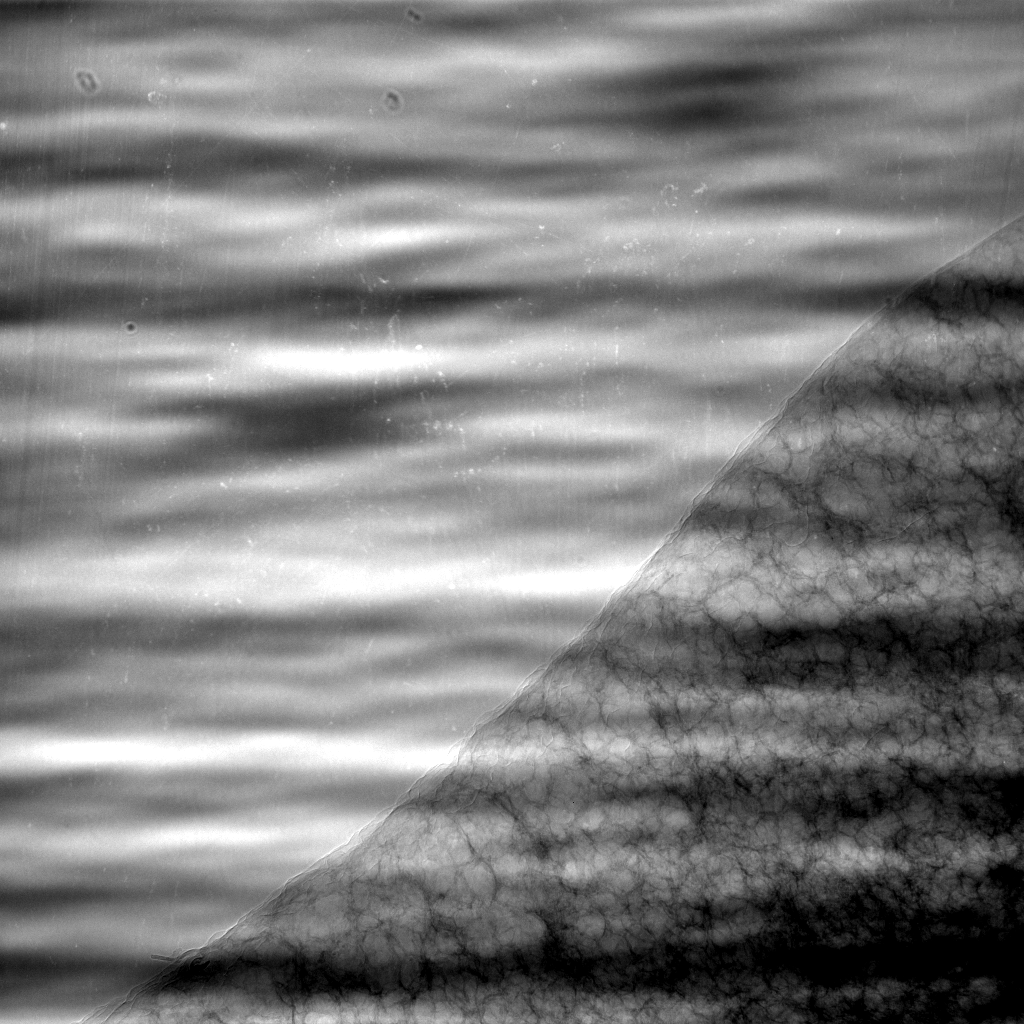
\includegraphics[width=\imagewidth]{R108C21Cb_s13358_normalize}};%
				\def\overlap{141}%
				\fill [red, nearly transparent] (1024-\overlap,1) rectangle (1024,1024);%
				\draw (1024-\overlap,1) rectangle (1024,1024);%
			\end{tikzpicture}%
			\begin{tikzpicture}[x=\imagescale,y=-\imagescale]%
				\node[anchor=north west,inner sep=0pt,outer sep=0pt] at (0,0)%
					{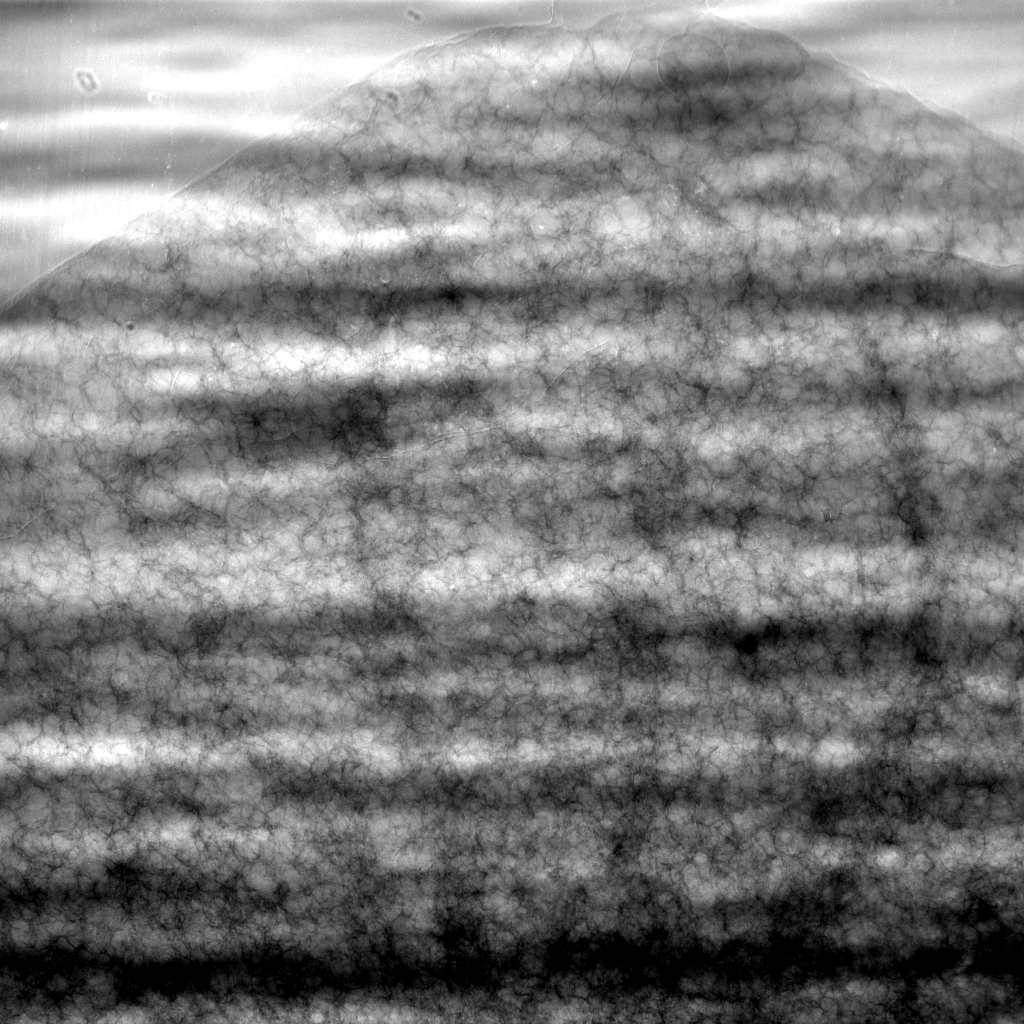
\includegraphics[width=\imagewidth]{R108C21Cb_s23358_normalize}};%
				\def\overlap{141}%
				\fill [green, nearly transparent] (1,1) rectangle (\overlap,1024);%
				\draw (1,1) rectangle (\overlap,1024);%
				\def\overlap{138}%
				\fill [blue, nearly transparent] (1024-\overlap,1) rectangle (1024,1024);%
				\draw (1024-\overlap,1) rectangle (1024,1024);%
			\end{tikzpicture}%
			\begin{tikzpicture}[x=\imagescale,y=-\imagescale]%
				% place image (integer coordinates refer to pixel centers):
				\node[anchor=north west,inner sep=0pt,outer sep=0pt] at (0,0)%
					{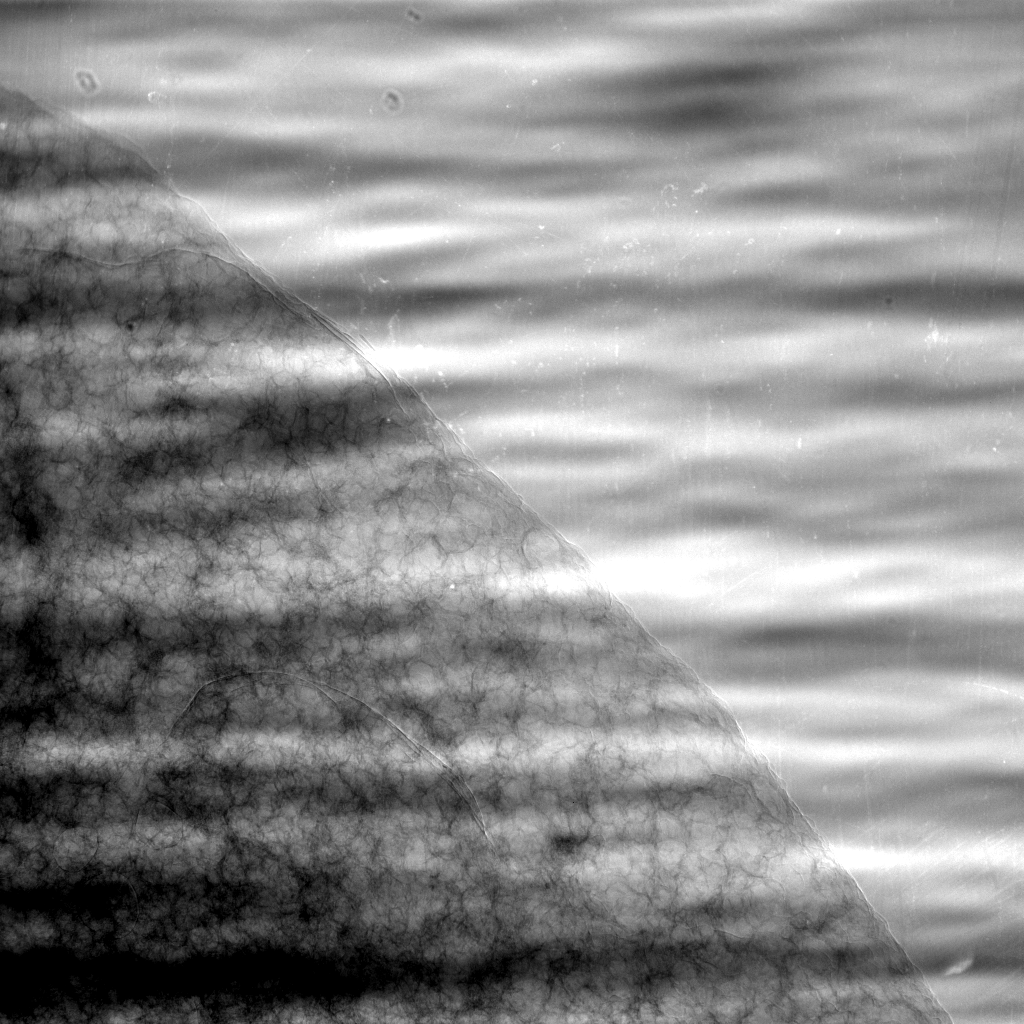
\includegraphics[width=\imagewidth]{R108C21Cb_s33358_normalize}};%
				\def\overlap{138}%
				\fill [yellow, nearly transparent] (1,1) rectangle (\overlap,1024);%
				\draw (1,1) rectangle (\overlap,1024);%
				\draw[|-|,color=white] (1,200) -- (1024,200) node [midway,above] {\SI{1.51552}{\milli\meter}};%
				\def\x{924}% 1024 - 100
				\def\y{922}% 1024 * .9 = 921.6
				\def\bar{338}% 100 px = 148 um
				\draw[|-|,color=white] (\x-\bar,\y) -- (\x,\y) node [midway,above] {\SI{500}{\micro\meter}};%
			\end{tikzpicture}%
			\label{fig:subscans}%
			}\\%
		\renewcommand{\imsize}{\linewidth}%
		\pgfmathsetlength{\imagewidth}{\imsize} % desired displayed width of image
		\pgfmathsetlength{\imagescale}{\imagewidth/2793}% pixel width of image
		\subfloat[Merged and corrected image from the three subscans shown in subfigure~\subref{fig:subscans}. Each merged projection has a size of 2793\(\times\)1024 pixels at a resolution of \SI{1.48}{\micro\meter\per pixel}. The width of the merged projections is slightly smaller than three times the width of the subscans due to the overlap needed to merge the projections (2793~px$=3\cdot3072$~px$-141$~px$-138$~px). Since the x-ray beam is extremely stable, the bands visible in the raw projections can be eliminated.]{%
			\begin{tikzpicture}[x=\imagescale,y=-\imagescale]%
				\node[anchor=north west,inner sep=0pt,outer sep=0pt] at (0,0)%
					{\includegraphics[width=\imagewidth]{R108C21Cb_mrg3333_normalize}};%
				\def\x{2693} % 2793-100
				\def\y{922} % 1024*.9 = 921.6
				\def\bar{338} % 100 px = 148 um
				\draw[|-|,color=white] (1,256) -- (2792,256) node [midway,above] {\SI{4.13364}{\milli\meter}};
				\draw[|-|,color=white] (\x-\bar,\y) -- (\x,\y) node [midway,above] {\SI{500}{\micro\meter}};
				\end{tikzpicture}%
			\label{fig:merge-proj}%
			}\\%
		\renewcommand{\imsize}{\linewidth}%
		\pgfmathsetlength{\imagewidth}{\imsize}% desired displayed width of image
		\pgfmathsetlength{\imagescale}{\imagewidth/2792}% pixel width of image (image has been resized from 2994*1123, so that scalebar is at the same height without calculating too much...)
		\subfloat[Cropped part of one slice of the tomographic dataset reconstructed from 5244 merged projections shown in subfigure~\subref{fig:merge-proj}. Due to the coherence of the x-ray beam the air-to-paraffin interface is visible around the sample.]{%
			\begin{tikzpicture}[x=\imagescale,y=-\imagescale]%
				% place image (integer coordinates refer to pixel centers):
				\node [anchor=north west,inner sep=0pt,outer sep=0pt] at (0,0)%
					{\includegraphics[width=\imagewidth]{R108C21Cb_mrg1024rec8bit}};% ``mogrify -shave 0x900 -normalize -format png R108C21Cb_mrg1024rec8bit.tif''
				\clip (0,0) rectangle (2792,992);				
				\def\x{2692} % 2708-100
				\def\y{893} % 992 * .9 = 892.8
				\def\bar{338} % 100 px = 148 um
				%%%% scalebar
					\draw[|-|,color=white] (\x-\bar,\y) -- (\x,\y) node [midway,above] {\SI{500}{\micro\meter}};
					\draw[|-|,color=white] (1,20) -- (2792,20) node [midway,below] {\SI{4.13216}{\milli\meter}};
				%%%% center
					\fill [color=red] (2792/2,992/2) circle (5);
				%%%% big circle
					\draw [dashed,color=red] (2792/2,992/2) circle (512);
					\def\angle{45}
					\draw [white,<->] (2792/2,992/2) +(\angle:0) --  node (bigto) {} +(\angle:512); 
					\node [white] (bigfrom) at (256,256){$\frac{1024}{2}$px};
					\draw [white,->,densely dotted] (bigfrom) to [bend left=45] (bigto);
				%%%% big circle
				%%%% 141px circle
				\draw [dashed,color=red] (2792/2,992/2) circle (512-141);
				\def\angle{45+90}
					\draw [white,<->] (2792/2,992/2) +(\angle:0) -- node (smallto) {} +(\angle:512-141);
					\node [white] (smallfrom) at (256,384) {$\frac{1024}{2}-141$px};
					\draw [white,->,densely dotted] (smallfrom) to [bend left=45] (smallto);
				%%%% 141px circle					
%				%%%% 138px circle
%				\draw [dashed,color=red] (2792/2,992/2) circle (512-138);
%				\def\angle{45+90+90}
%					\draw [white,<->] (2792/2,992/2) +(\angle:0) -- node (vsmallto) {} +(\angle:512-138);
%					\node [white] (vsmallfrom) at (2972-768,992-512) {$\frac{1024}{2}-138$px};
%					\draw [white,->,densely dotted] (vsmallfrom) to [bend right=45] (vsmallto);
%				%%%% 138px circle
				%%%% inset
%				\newcommand{\size}{.2\imagewidth}%
%				\clip (256,256) rectangle (512,512);
%				\node[anchor=north west,inner sep=0pt,outer sep=0pt] at (0,0)
%					{\includegraphics[width=\size]{R108C21Cb_mrg1024rec8bit}};
%					\draw[white] (0,0) rectangle (\size,-\size);
				%%%% inset
				\end{tikzpicture}%
			\label{fig:merge-rec}%
			}%
%%%%%%%%%%%%%%%%%%%%%%%%%%%%%	
%	\caption{caption}
%\end{figure}
%\end{document}
%	\caption{Wide field scan of a rat lung sample obtained from a Sprague-Dawley rat 21 days after birth, showing the distal-medial edge of the right lower lung lobe. The sample has been scanned at \SI{12.6}{\kilo\electronvolt}, the protocol details conform to protocol ``B'', described in table~\ref{tab:protocols}.}%
%	\label{fig:wide field scan results}%
%	\todo[inline]{this figure is much too big to fit on one page, but it's very hard to scale down. what can we do?}%
%	\todo[inline]{!!!ALL subsequent 3D-figures have ``strange'' scale bars on them. The long scale bars are there so YOU can control my work, the short scale bars are the correct ones!!!}%
%\end{figure*}
%%% normal figures %%%


\subsection{Increasing the FOV}


With the FOV available up to now at TOMCAT we have only been able to fit partial acini inside our datasets. Increasing the available FOV three times allows us to obtain three dimensional reconstructions of acini only restricted by the available sample size, but not by the FOV of the imaging method. From figure~\ref{subfig:overview-merge} it appears clearly that the FOV is increased, allowing the visualization of third acinus (yellow) which is not visible inside the FOV of a conventional scan (figure~\ref{subfig:overview-s2}). Additionally, it is also visible that both the red and green segment for the conventional scan are extend out of the FOV of the conventional scan, we need to record a wide field scan to visualize both these segments in three dimensions, as can be seen in figure~\ref{subfig:overview-merge}. The red and yellow segment visualized for the wide field scan are still only partial acini, but their size is only limited by the dimensions of the lung sample, not by the imaging method.

The data obtained from wide field scanning permits the visualizations of entire acini inside the rat lung and will help to gain a deep insight into the postnatal structural lung development, see section~\ref{sec:outlook}.


%%% iucr %%%
%\onecolumn
\begin{figure}%
	\centering%
	\caption{Three dimensional visualization of the distal-medial tip of the right lower lung lobe of a Sprague Dawley rat. The gray structure in the background shows a semitransparent view of the sample with segmented airways. The foreground shows isosurfaces of terminal airways that have been extracted using a threshold interval based region growing algorithm. a): Conventional scan; the extracted acini (green and red segments) contain only partial. b): Wide field scan; the green and red segment show multiple acini fully inside the dataset, the yellow segment contains a partial acinus. The segmentation is only limited by the sample size and not by the FOV of the tomographic scan.}%
	\def\x{250}%
	\def\y{575}%
	\begin{tabular}{p{.75\linewidth}p{.75\linewidth}}%
		\renewcommand{\imsize}{\linewidth}%
		\pgfmathsetlength{\imagewidth}{\imsize}%
		\pgfmathsetlength{\imagescale}{\imagewidth/1202}%
		\begin{tikzpicture}[x=\imagescale,y=-\imagescale]%
			\node[anchor=north west,inner sep=0pt,outer sep=0pt] at (0,0)%
				{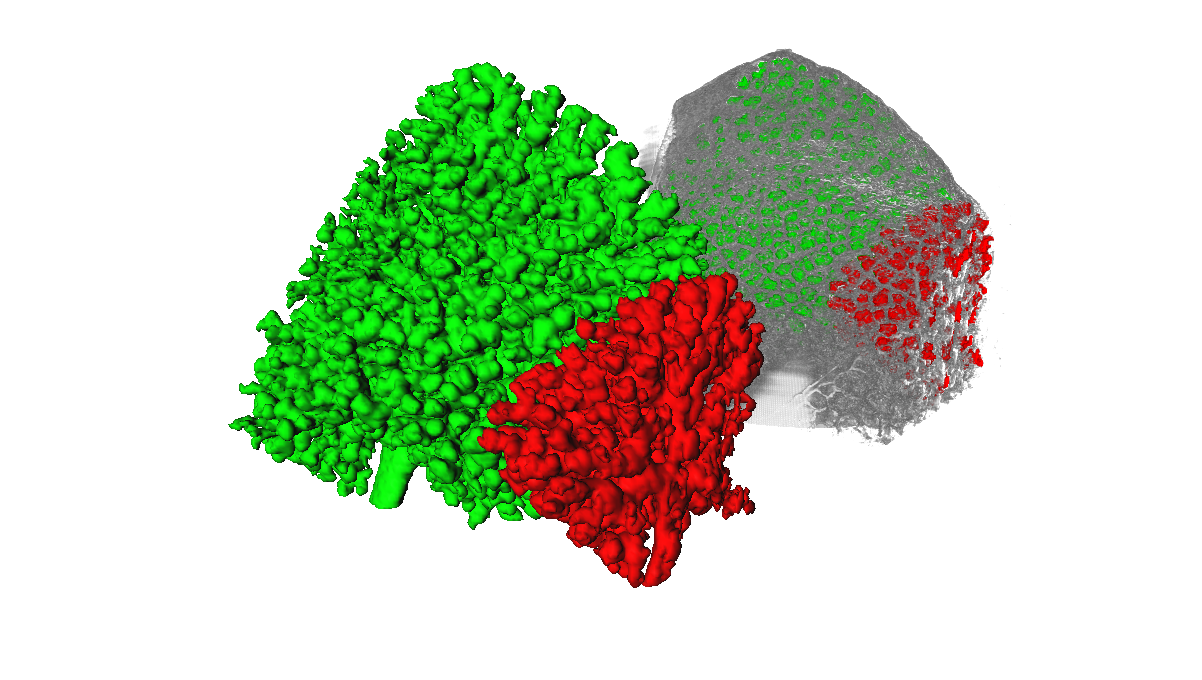
\includegraphics[width=\imagewidth]{img/widefieldscanning/R108C04C-overview-s2}};%
			% 510px = 1.5155mm > 100px = 297um > 168px = 500um
			\draw[|-|,thick] (244,367) -- (718,554) node [sloped,midway,above] {\SI{1.5155}{\milli\meter}};%
			\draw[|-|,thick] (\x,\y) -- (\x+168,\y) node [midway,above] {\SI{500}{\micro\meter}};%
		\end{tikzpicture}%
		\label{subfig:overview-s2}%
	\\%
	a) Conventional scan\\%
	\\%
		\renewcommand{\imsize}{\linewidth}%
		\pgfmathsetlength{\imagewidth}{\imsize}%
		\pgfmathsetlength{\imagescale}{\imagewidth/1202}%
	\def\x{150}%
	\def\y{575}%
		\label{subfig:overview-merge}%
		\begin{tikzpicture}[x=\imagescale,y=-\imagescale]%
			\node[anchor=north west,inner sep=0pt,outer sep=0pt] at (0,0)%
				{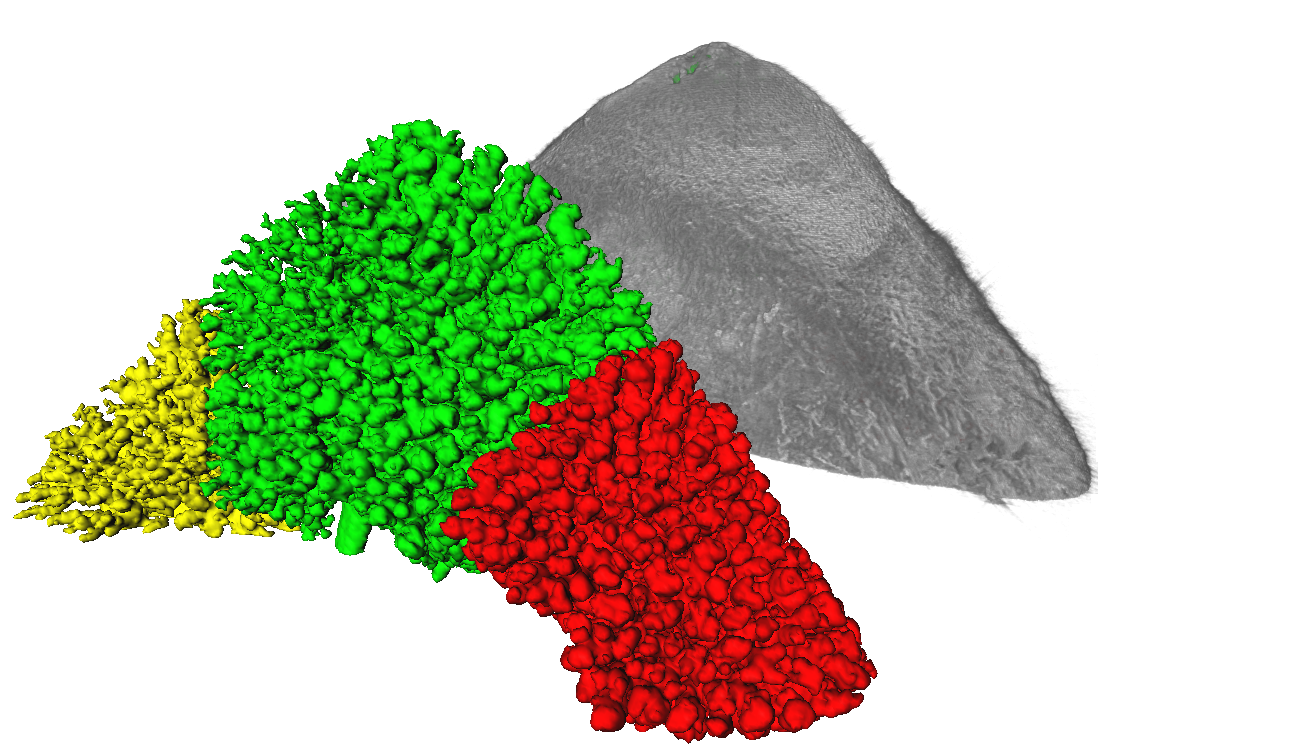
\includegraphics[width=\imagewidth]{img/widefieldscanning/R108C04C-overview-merge}};%
			% 906px = 4.0641mm > 100px = 449um > 111px = 500um
			\draw[|-|,thick] (39,454) -- (923,653) node [sloped,midway,above] {\SI{4.0641}{\milli\meter}};%
			\draw[|-|,thick] (\x,\y) -- (\x+222,\y) node [midway,above] {\SI{1}{\milli\meter}};%
		\end{tikzpicture}\\%
	b) Scan with increased FOV\\%
	\end{tabular}%
	\label{fig:FOV increase overview}%
\end{figure}%
%\twocolumn
%%% iucr %%%
%%% normal figures %%%
%\begin{figure*}[htp]%
%\renewcommand{\imsize}{\linewidth}%
%\pgfmathsetlength{\imagewidth}{\imsize}% desired displayed width of image
%\pgfmathsetlength{\imagescale}{\imagewidth/1202}% pixel width of imagefile used below
%	\centering%
%	\def\x{250}%
%	\def\y{575}%
%	\subfloat[Conventional scan]{%
%		\label{subfig:overview-s2}%
%		\begin{tikzpicture}[x=\imagescale,y=-\imagescale]
%			\node[anchor=north west,inner sep=0pt,outer sep=0pt] at (0,0)
%				{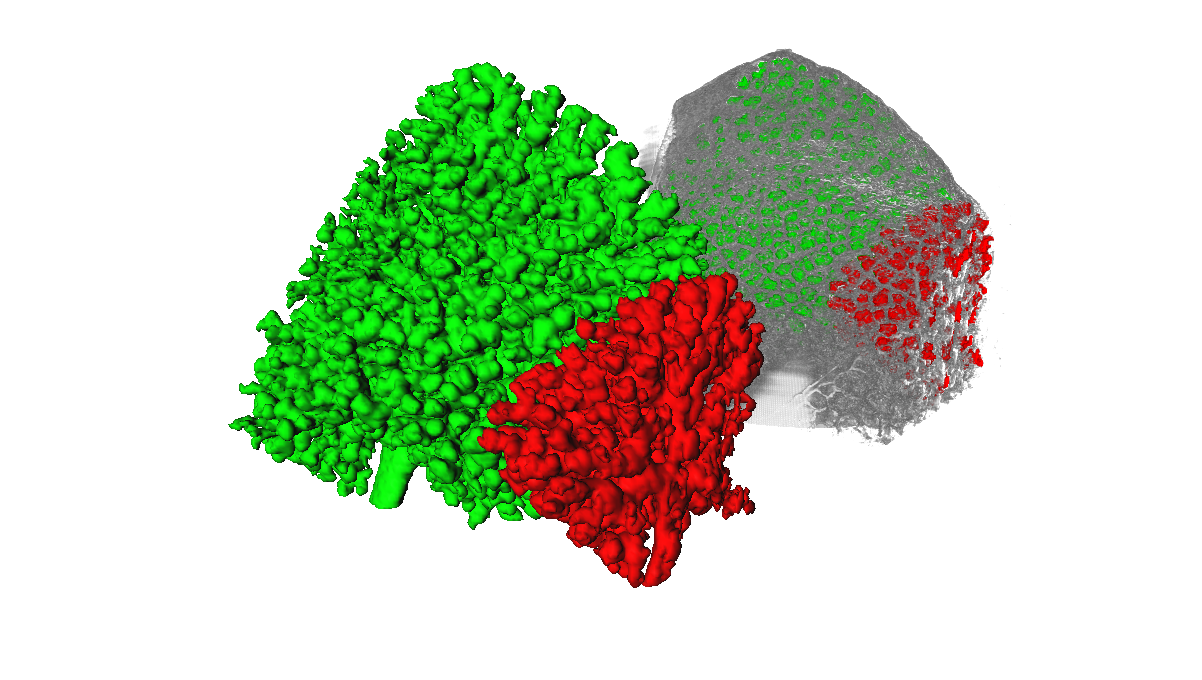
\includegraphics[width=\imagewidth]{img/widefieldscanning/R108C04C-overview-s2}};
%			% 510px = 1.5155mm > 100px = 297um > 168px = 500um
%			\draw[|-|,thick] (244,367) -- (718,554) node [sloped,midway,above] {\SI{1.5155}{\milli\meter}};
%			\draw[|-|,thick] (\x,\y) -- (\x+168,\y) node [midway,above] {\SI{500}{\micro\meter}};
%		\end{tikzpicture}%
%	}\\%
%	\def\x{150}%
%	\def\y{575}%
%	\subfloat[Scan with increased FOV]{%
%		\label{subfig:overview-merge}%
%		\begin{tikzpicture}[x=\imagescale,y=-\imagescale]
%			\node[anchor=north west,inner sep=0pt,outer sep=0pt] at (0,0)
%				{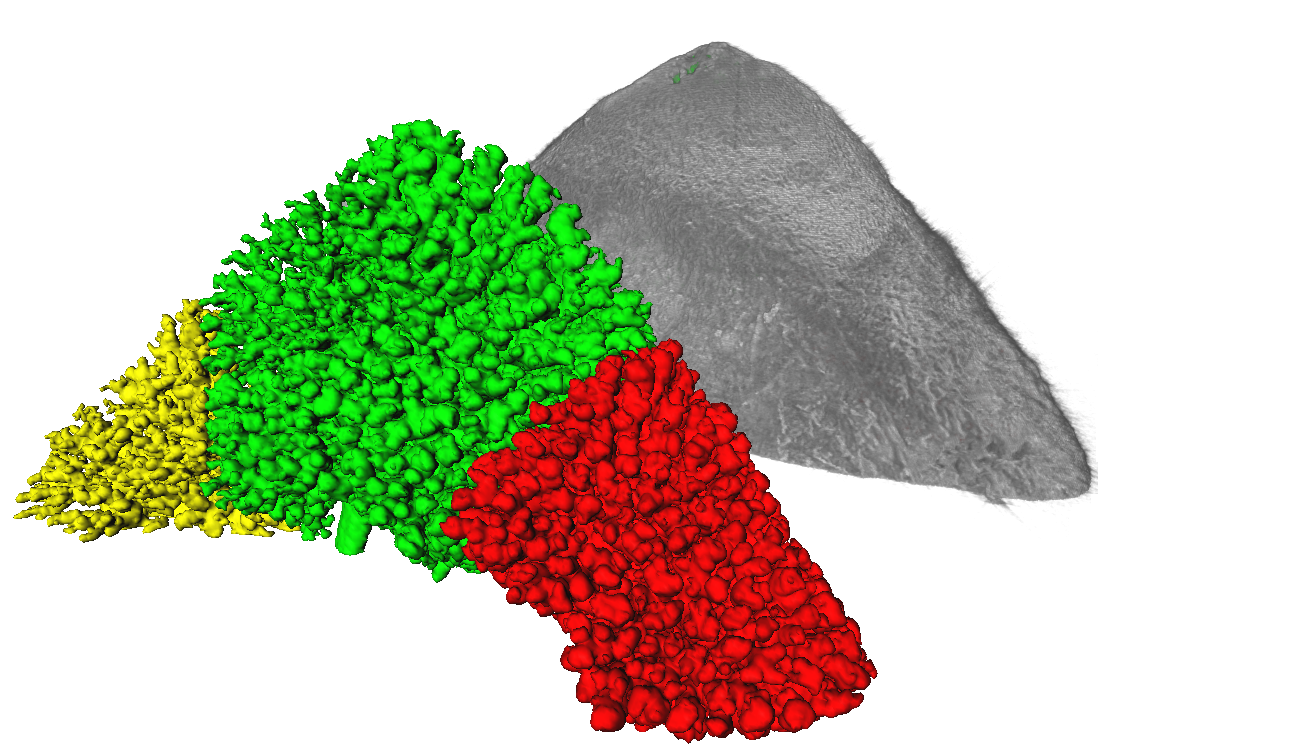
\includegraphics[width=\imagewidth]{img/widefieldscanning/R108C04C-overview-merge}};
%			% 906px = 4.0641mm > 100px = 449um > 111px = 500um
%			\draw[|-|,thick] (39,454) -- (923,653) node [sloped,midway,above] {\SI{4.0641}{\milli\meter}};
%			\draw[|-|,thick] (\x,\y) -- (\x+222,\y) node [midway,above] {\SI{1}{\milli\meter}};
%		\end{tikzpicture}%
%	}%
%%	\caption[3D visualization of the right lower lung lobe of a Sprague Dawley rat]
%	\caption{Three dimensional visualization of the distal-medial tip of the right lower lung lobe of a Sprague Dawley rat. The gray structure in the background shows a semitransparent view of the sample with segmented airways. The foreground shows isosurfaces of terminal airways that have been extracted using a threshold interval based region growing algorithm. \subref{subfig:overview-s2}: Conventional scan; the extracted acini (green and red segments) contain only partial. \subref{subfig:overview-merge}: Wide field scan; the green and red segment show multiple acini fully inside the dataset, the yellow segment contains a partial acinus. The segmentation is only limited by the sample size and not by the FOV of the tomographic scan.}%
%	\label{fig:FOV increase overview}%
%\end{figure*}
%%% normal figures %%%

\subsection{Quality guided protocols}%
A sequence of 19 protocols with varying quality has been scanned to assess the predictions obtained through preliminary simulations and to assess the plot that is presented to choose a scanning protocol suited for the demands on scanning time and reconstruction quality, as defined in section~\ref{subsec:wfs-setup}.

Differences between the protocols have been calculated using the difference image of binarized slices, segmented according to~\citeasnoun{Otsu1979}. The binarization of the images suppresses small variations in the gray values which occur through slight variation in the beam profile during the acquisition of the individual subscans, and enables us to only take into account the pixels that are differ between the 19 different protocols.

The difference value ($E_{norm}$) plotted in figure~\ref{fig:NormalizedErrorPlot} has been calculated for each protocol $i=$1--19 according to equations~\ref{eq:errorcalculation-a}--\ref{eq:errorcalculation-c}. Using a thresholded slice $i$ of each protocol $Prot$ ($Slice_{Prot_{i}}$) and the corresponding slice $i$ of the gold standard protocol $B$ ($Slice_{B_{i}}$) we calculated the absolute difference image ($D_{Prot_{i}}$) of these two slices $i$. The sum of all pixels of this difference image yields a value ($E_{Prot_{norm_{i}}}$) for each slice $i$ of each Protocol $Prot$, which assesses the difference of the examined slice with the corresponding slice of the gold standard protocol. 

\begin{eqnarray}%
	D_{Prot_{i}} &=& |Slice_{B_{i}}-Slice_{Prot_{i}}|\label{eq:errorcalculation-a}\\%
	E_{Prot_{norm_{i}}} &=& \sum_{x}\sum_{y} D_{Prot_{i}}\label{eq:errorcalculation-b}\\%
    E_{Prot_{norm}} &=& \overline{E_{Prot_{norm_{i}}}}\label{eq:errorcalculation-c}%
\end{eqnarray}%

Such a combined difference value ($E_{Prot_{norm_{i}}}$) has been calculated for 205 regularly spaced slices ($i=1:5:1024$) of the full dataset. The mean ($\overline{E_{Prot_{norm_{i}}}}$) difference value for all slices has been normalized to the scanned quality-steps from 20--\SI{100}{\percent} (as stated in table~\ref{tab:protocols}) and plotted as max$(E_{norm}-E_{Prot_{norm}})$ with its standard deviation ($\sigma(E_{Prot_{norm_{i}}})$), as can be seen in figure~\ref{fig:NormalizedErrorPlot}. The normalization and inversion has been done to make the plotted values directly comparable with the plotted simulated qualities shown in figure~\ref{fig:qualityplot}.

The calculated quality of the reconstructions from the different protocols decreases with decreasing amount of total obtained projections, as expected. Figure~\ref{fig:NormalizedErrorPlot} shows a plot of the calculated error of the different protocols compared to a gold standard protocol (blue diamonds), those are experimental results not derived using simulations with a phantom, but real data obtained from actual scans of lung tissue. Overlaid on this plot are the data obtained from simulations (red dots). Both the plots for the simulation and the normalized difference value are not perfectly in agreement, but show the same trend. The simulation shows an exponential decrease in quality, while the calculated, normalized error show a more linear decrease in quality from protocol B towards protocol T.

%%% iucr %%%
\begin{figure}%
	\centering%
	\caption{Plot of normalized difference Value ($E_{norm}$, blue diamonds) for the 19 scanned protocols overlaid over Quality-plot (red dots) obtained from the simulation. The normalized Error has been calculated in such a way that we calculated the difference image for Protocol $i$ compared to Protocol B. The error bars for each protocol show the standard deviation of the error which was calculated for 205 of the 1024 slices for each protocol. Note that the scale of the error been normalized to 20--\SI{100}{\percent}, so that both the quality from the simulation and the error are directly comparable. The abscissa shows the scanning time in percentage of time used for the gold standard scan. The protocols would be shown are in decreasing order from T--B for increasing percentage.}%
	%\documentclass{article}
%\usepackage{tikz,pgfplots}
%\usepackage[pdftex,active,tightpage]{preview}
%\begin{document}
%\begin{preview}
%%%%%%%%%%%%%%%%%%%%%%%%%%%%%%
\begin{tikzpicture}

\pgfplotsset{every axis legend/.append style={at={(0.8,0.08)},anchor=base}}

\begin{axis}[%
	xmajorgrids,
  ymajorgrids,
	width=\linewidth,
	height=0.618\linewidth,
	%scale only axis,
	%xmin=0,%xmax=129,
	ymin=0,%ymax=125,
  xlabel={Scanning Time [\%\ of Gold Standard]},%
	ylabel={Expected Quality [\%], Quality$-E_{i_{norm}}$}%
	]

% Protocols
\addplot [ fill=red, only marks, mark = *]
	coordinates{
		(16.14,20)
		(19.37,21.2284)
		(29.08,46.0522)
		(32.29,54.5201)
		(38.75,60.7072)
		(40.37,61.8107)
		(48.46,67.4167)
		(48.43,68.7811)
		(58.12,71.8724)
		(56.52,75.28)
		(67.83,76.1345)
		(64.58,80.1592)
		(77.49,78.0612)
		(72.67,83.9645)
		(87.20,80.4284)
		(80.72,86.6889)
		(96.87,84.9458)
		(96.84,89.1421)
		(116.24,100)
};

\addplot [domain=16.14:116.24,color=red, semitransparent,ultra thick]
	{0.6936*x+26.891}; 

%% Line plot
%\addplot [smooth, solid, semitransparent]
	%coordinates{
		%(16.14,16.8548)
		%(19.37,25.9575)
		%(29.08,46.6567)
		%(32.29,51.7347)
		%(38.75,59.9714)
		%(40.37,61.6854) 
		%(48.46,68.6146)
		%(48.43,68.6305) 
		%(56.52,73.5452)
		%(58.12,74.3455)
		%(64.58,77.1605)
		%(67.83,78.3754)
		%(72.67,80.0091)
		%(77.49,81.5005)
		%(80.72,82.4599)
		%(87.20,84.3973)
		%(96.87,87.719)
%%		(96.87,87.719)
		%(116.24,99.8565)
%};

\addplot [ color=blue, only marks, mark=diamond ]
plot [ error bars/.cd, y dir=both, y explicit ]
    coordinates{
	( 16.14,20.0000) +- (0,0)      % T
	( 19.37,38.1358) +- (0,3.1135) % S
	( 29.08,30.2919) +- (0,1.3958) % R
	( 32.29,42.2255) +- (0,2.5278) % Q
	( 38.75,49.2247) +- (0,7.6789) % P
	( 40.37,53.0181) +- (0,6.8507) % O 
	( 48.46,41.5079) +- (0,4.7824) % N  
	( 48.43,51.6990) +- (0,4.7110) % M
	( 58.12,49.9058) +- (0,9.1839) % L
	( 56.52,66.1100) +- (0,8.1635) % K
	( 67.83,50.4137) +- (0,5.5671) % J
	( 64.58,56.2138) +- (0,3.2329) % I
	( 77.49,60.0243) +- (0,8.0805) % H
	( 72.67,65.7727) +- (0,6.2214) % G
	( 87.20,55.0069) +- (0,4.1882) % F
	( 80.72,79.6708) +- (0,3.0107) % E
	( 96.87,70.4018) +- (0,3.0863) % D
	( 96.87,74.3991) +- (0,6.8125) % C
	(116.24,99.8987) +- (0,1.3487) % B
};

\addplot [domain=16.14:116.24,color=blue, semitransparent,ultra thick]
	{0.5833*x+20.226}; 

\legend{%
	Simulation,%
	linear Interpolation,%
	$E_{i_{norm}}$,%
	linear Interpolation}

% \draw [<-] (axis cs:97.87,74.3991) -- (axis cs:99.87,74.3991) node [anchor=text] {\tiny C}; 
% \draw [<-] (axis cs:97.87,70.4018) -- (axis cs:99.87,70.4018) node [anchor=text] {\tiny D};
% \draw [<-] (axis cs:81.72,79.6708) -- (axis cs:82.72,79.6708) node [anchor=text] {\tiny E};
% \draw [<-] (axis cs:78.49,60.0243) -- (axis cs:79.49,60.0243) node [anchor=text] {\tiny H};
% \draw [<-] (axis cs:65.58,56.2138) -- (axis cs:66.58,56.2138) node [anchor=text] {\tiny I};
% \draw [<-] (axis cs:49.43,51.6990) -- (axis cs:51.43,51.6990) node [anchor=text] {\tiny M};
% \draw [<-] (axis cs:49.46,41.5079) -- (axis cs:51.46,41.5079) node [anchor=text] {\tiny N};

\tikzstyle{every pin}=[pin distance=2ex,font=\scriptsize]
\node[coordinate, pin=below right:{B}] at (axis cs:116.24,99.8987) {}; % B
\node[coordinate, pin=-22.5:{C}] at (axis cs:96.87,74.3991) {}; % C
\node[coordinate, pin=below right:{D}] at (axis cs:96.87,70.4018) {}; % D
\node[coordinate, pin=-5:{E}] at (axis cs:80.72,79.6708) {}; % E
\node[coordinate, pin=below right:{F}] at (axis cs:87.20,55.0069) {}; % F
\node[coordinate, pin=above right:{G}] at (axis cs:72.67,65.7727) {}; % G
\node[coordinate, pin=below right:{H}] at (axis cs:77.49,60.0243) {}; % H
\node[coordinate, pin=above right:{I}] at (axis cs:64.58,56.2138) {}; % I
\node[coordinate, pin=below right:{J}] at (axis cs:67.83,50.4137) {}; % J
\node[coordinate, pin=right:{K}] at (axis cs:56.52,66.1100) {}; % K
\node[coordinate, pin=below right:{L}] at (axis cs:58.12,49.9058) {}; % L
\node[coordinate, pin=above right:{M}] at (axis cs:48.43,51.6990) {}; % M
\node[coordinate, pin=below right:{N}] at (axis cs:48.46,41.5079) {}; % N  
\node[coordinate, pin=above right:{O}] at (axis cs:40.37,53.0181) {}; % O
\node[coordinate, pin=below right:{P}] at (axis cs:38.75,49.2247) {}; % P
\node[coordinate, pin=below right:{Q}] at (axis cs:32.29,42.2255) {}; % Q
\node[coordinate, pin=below right:{R}] at (axis cs:29.08,30.2919) {}; % R
\node[coordinate, pin=right:{S}] at (axis cs:19.37,38.1358) {}; % S
\node[coordinate, pin=below right:{T}] at (axis cs:16.14,20.0000) {}; % T

\node[coordinate, pin=above left:{$R^2=0.8287$}] at (axis cs:106.24,100.5791) {};
\node[coordinate, pin=below right:{$R^2=0.7868$}] at (axis cs:106.24, 82.1958) {};


\end{axis}

\end{tikzpicture}
%%%%%%%%%%%%%%%%%%%%%%%%%%%%%%
%\end{preview}
%\end{document}

%%%%%%%%%%%%%%%%%%%%%%%%%%%%%%
% plot erstellt mit MATLAB-File p:\\MATLAB\WideFieldScan/Paper/wfs_Compare2008c_ErrorPlot.m
% mit FromToTo = 1:5:1024
% sowie matlab2tikz
% Daten
%%%%%%%%%%Time =
%%%%%%%%%%  Columns 1 through 12
%%%%%%%%%%
%%%%%%%%%%   13.75   16.50   24.77   27.50   33   34.38   41.27   41.25   49.50   48.14   57.77   55
%%%%%%%%%%
%%%%%%%%%%  Columns 13 through 19
%%%%%%%%%%
%%%%%%%%%%   66   61.89   74.27   68.75   82.50   82.50   99.01
%MeanCumulativeError =
%
%  Columns 1 through 12
%
%   20.0000   38.1358   30.2919   42.2255   49.2247   53.0181   41.5079   51.6990   49.9058   66.1100   50.4137   56.2138
%
%  Columns 13 through 19
%
%   60.0243   65.7727   55.0069   79.6708   70.4018   74.3991   99.8987
%
%
%StandardDeviationofCumulativeError =
%
%  Columns 1 through 12
%
%         0    3.1135    1.3958    2.5278    7.6789    6.8507    4.7824    4.7110    9.1839    8.1635    5.5671    3.2329
%
%  Columns 13 through 19
%
%    8.0805    6.2214    4.1882    3.0107    3.0863    6.8125    1.3487
%%%%%%%%%%%%%%%%%%%%%%%%%%%%%%%
	\label{fig:NormalizedErrorPlot}%
\end{figure}%
%%% iucr %%%
%%% normal figures %%%
%%\begin{figure*}[htp]
%%	\centering
%%	%\documentclass{article}
%\usepackage{tikz,pgfplots}
%\usepackage[pdftex,active,tightpage]{preview}
%\begin{document}
%\begin{preview}
%%%%%%%%%%%%%%%%%%%%%%%%%%%%%%
\begin{tikzpicture}

\pgfplotsset{every axis legend/.append style={at={(0.8,0.08)},anchor=base}}

\begin{axis}[%
	xmajorgrids,
  ymajorgrids,
	width=\linewidth,
	height=0.618\linewidth,
	%scale only axis,
	%xmin=0,%xmax=129,
	ymin=0,%ymax=125,
  xlabel={Scanning Time [\%\ of Gold Standard]},%
	ylabel={Expected Quality [\%], Quality$-E_{i_{norm}}$}%
	]

% Protocols
\addplot [ fill=red, only marks, mark = *]
	coordinates{
		(16.14,20)
		(19.37,21.2284)
		(29.08,46.0522)
		(32.29,54.5201)
		(38.75,60.7072)
		(40.37,61.8107)
		(48.46,67.4167)
		(48.43,68.7811)
		(58.12,71.8724)
		(56.52,75.28)
		(67.83,76.1345)
		(64.58,80.1592)
		(77.49,78.0612)
		(72.67,83.9645)
		(87.20,80.4284)
		(80.72,86.6889)
		(96.87,84.9458)
		(96.84,89.1421)
		(116.24,100)
};

\addplot [domain=16.14:116.24,color=red, semitransparent,ultra thick]
	{0.6936*x+26.891}; 

%% Line plot
%\addplot [smooth, solid, semitransparent]
	%coordinates{
		%(16.14,16.8548)
		%(19.37,25.9575)
		%(29.08,46.6567)
		%(32.29,51.7347)
		%(38.75,59.9714)
		%(40.37,61.6854) 
		%(48.46,68.6146)
		%(48.43,68.6305) 
		%(56.52,73.5452)
		%(58.12,74.3455)
		%(64.58,77.1605)
		%(67.83,78.3754)
		%(72.67,80.0091)
		%(77.49,81.5005)
		%(80.72,82.4599)
		%(87.20,84.3973)
		%(96.87,87.719)
%%		(96.87,87.719)
		%(116.24,99.8565)
%};

\addplot [ color=blue, only marks, mark=diamond ]
plot [ error bars/.cd, y dir=both, y explicit ]
    coordinates{
	( 16.14,20.0000) +- (0,0)      % T
	( 19.37,38.1358) +- (0,3.1135) % S
	( 29.08,30.2919) +- (0,1.3958) % R
	( 32.29,42.2255) +- (0,2.5278) % Q
	( 38.75,49.2247) +- (0,7.6789) % P
	( 40.37,53.0181) +- (0,6.8507) % O 
	( 48.46,41.5079) +- (0,4.7824) % N  
	( 48.43,51.6990) +- (0,4.7110) % M
	( 58.12,49.9058) +- (0,9.1839) % L
	( 56.52,66.1100) +- (0,8.1635) % K
	( 67.83,50.4137) +- (0,5.5671) % J
	( 64.58,56.2138) +- (0,3.2329) % I
	( 77.49,60.0243) +- (0,8.0805) % H
	( 72.67,65.7727) +- (0,6.2214) % G
	( 87.20,55.0069) +- (0,4.1882) % F
	( 80.72,79.6708) +- (0,3.0107) % E
	( 96.87,70.4018) +- (0,3.0863) % D
	( 96.87,74.3991) +- (0,6.8125) % C
	(116.24,99.8987) +- (0,1.3487) % B
};

\addplot [domain=16.14:116.24,color=blue, semitransparent,ultra thick]
	{0.5833*x+20.226}; 

\legend{%
	Simulation,%
	linear Interpolation,%
	$E_{i_{norm}}$,%
	linear Interpolation}

% \draw [<-] (axis cs:97.87,74.3991) -- (axis cs:99.87,74.3991) node [anchor=text] {\tiny C}; 
% \draw [<-] (axis cs:97.87,70.4018) -- (axis cs:99.87,70.4018) node [anchor=text] {\tiny D};
% \draw [<-] (axis cs:81.72,79.6708) -- (axis cs:82.72,79.6708) node [anchor=text] {\tiny E};
% \draw [<-] (axis cs:78.49,60.0243) -- (axis cs:79.49,60.0243) node [anchor=text] {\tiny H};
% \draw [<-] (axis cs:65.58,56.2138) -- (axis cs:66.58,56.2138) node [anchor=text] {\tiny I};
% \draw [<-] (axis cs:49.43,51.6990) -- (axis cs:51.43,51.6990) node [anchor=text] {\tiny M};
% \draw [<-] (axis cs:49.46,41.5079) -- (axis cs:51.46,41.5079) node [anchor=text] {\tiny N};

\tikzstyle{every pin}=[pin distance=2ex,font=\scriptsize]
\node[coordinate, pin=below right:{B}] at (axis cs:116.24,99.8987) {}; % B
\node[coordinate, pin=-22.5:{C}] at (axis cs:96.87,74.3991) {}; % C
\node[coordinate, pin=below right:{D}] at (axis cs:96.87,70.4018) {}; % D
\node[coordinate, pin=-5:{E}] at (axis cs:80.72,79.6708) {}; % E
\node[coordinate, pin=below right:{F}] at (axis cs:87.20,55.0069) {}; % F
\node[coordinate, pin=above right:{G}] at (axis cs:72.67,65.7727) {}; % G
\node[coordinate, pin=below right:{H}] at (axis cs:77.49,60.0243) {}; % H
\node[coordinate, pin=above right:{I}] at (axis cs:64.58,56.2138) {}; % I
\node[coordinate, pin=below right:{J}] at (axis cs:67.83,50.4137) {}; % J
\node[coordinate, pin=right:{K}] at (axis cs:56.52,66.1100) {}; % K
\node[coordinate, pin=below right:{L}] at (axis cs:58.12,49.9058) {}; % L
\node[coordinate, pin=above right:{M}] at (axis cs:48.43,51.6990) {}; % M
\node[coordinate, pin=below right:{N}] at (axis cs:48.46,41.5079) {}; % N  
\node[coordinate, pin=above right:{O}] at (axis cs:40.37,53.0181) {}; % O
\node[coordinate, pin=below right:{P}] at (axis cs:38.75,49.2247) {}; % P
\node[coordinate, pin=below right:{Q}] at (axis cs:32.29,42.2255) {}; % Q
\node[coordinate, pin=below right:{R}] at (axis cs:29.08,30.2919) {}; % R
\node[coordinate, pin=right:{S}] at (axis cs:19.37,38.1358) {}; % S
\node[coordinate, pin=below right:{T}] at (axis cs:16.14,20.0000) {}; % T

\node[coordinate, pin=above left:{$R^2=0.8287$}] at (axis cs:106.24,100.5791) {};
\node[coordinate, pin=below right:{$R^2=0.7868$}] at (axis cs:106.24, 82.1958) {};


\end{axis}

\end{tikzpicture}
%%%%%%%%%%%%%%%%%%%%%%%%%%%%%%
%\end{preview}
%\end{document}

%%%%%%%%%%%%%%%%%%%%%%%%%%%%%%
% plot erstellt mit MATLAB-File p:\\MATLAB\WideFieldScan/Paper/wfs_Compare2008c_ErrorPlot.m
% mit FromToTo = 1:5:1024
% sowie matlab2tikz
% Daten
%%%%%%%%%%Time =
%%%%%%%%%%  Columns 1 through 12
%%%%%%%%%%
%%%%%%%%%%   13.75   16.50   24.77   27.50   33   34.38   41.27   41.25   49.50   48.14   57.77   55
%%%%%%%%%%
%%%%%%%%%%  Columns 13 through 19
%%%%%%%%%%
%%%%%%%%%%   66   61.89   74.27   68.75   82.50   82.50   99.01
%MeanCumulativeError =
%
%  Columns 1 through 12
%
%   20.0000   38.1358   30.2919   42.2255   49.2247   53.0181   41.5079   51.6990   49.9058   66.1100   50.4137   56.2138
%
%  Columns 13 through 19
%
%   60.0243   65.7727   55.0069   79.6708   70.4018   74.3991   99.8987
%
%
%StandardDeviationofCumulativeError =
%
%  Columns 1 through 12
%
%         0    3.1135    1.3958    2.5278    7.6789    6.8507    4.7824    4.7110    9.1839    8.1635    5.5671    3.2329
%
%  Columns 13 through 19
%
%    8.0805    6.2214    4.1882    3.0107    3.0863    6.8125    1.3487
%%%%%%%%%%%%%%%%%%%%%%%%%%%%%%
%%%	\caption[Plot of normalized difference value for the 19 scanned protocols]
%%	\caption{Plot of normalized difference Value ($E_{norm}$) for the 19 scanned protocols overlaid over Quality-plot obtained from the simulation. The normalized Error has been calculated in such a way that we calculated the difference image for Protocol $i$ compared to Protocol B. The error bars for each protocol show the standard deviation of the error which was calculated for 205 of the 1024 slices for each protocol. Note that the scale of the error been normalized to 20--\SI{100}{\percent}, so that both the quality from the simulation and the error are directly comparable. The abscissa shows the scanning time in percentage of time used for the gold standard scan. The protocols would be shown are in decreasing order from T--B for increasing percentage.}
%%	\label{fig:NormalizedErrorPlot}
%%\end{figure*}
%%% normal figures %%%

For protocols with the same total amount of projections, but different configurations of amount of projections for the central and the ring scan we see a difference in reconstruction quality (compare the marked protocols C and D as well as protocols M and N in figure~\ref{fig:NormalizedErrorPlot}). This difference arises through the fact that the differing amount of subscans acquired for the central and the subscan add up to the same total amount of projections, but contribute differently to the quality of the reconstruction. From this finding it seems desirable to choose a protocol with equal amounts of subscans for each of the three independent subscans instead of a protocol with the same total amount of projections, but a decreased amount of projections for the central scan. Since a reduced amount of projections for the central scan decrease the reconstruction quality for the central parts of the sample, this explanation seems natural. Additionally, the interpolation of missing projections could introduce artifacts in the reconstruction which are suppressed when simply stitching projections without interpolation.

\subsubsection{Three dimensional visualization of different protocols}%
\label{subsec:comparison}%
The 19 different protocols have been three dimensionally visualized and analyzed using MeVisLab (Version 1.6.1 (2008-09-21 Release), MeVis Medical Solutions AG, Bremen, Germany). Using a region growing algorithm~\cite{wiki:regiongrowing}, airway segments have been extracted from the tomographic dataset.  A seed point for the region growing algorithm has been manually defined inside the airway lumen to extract connected airway segments inside the tomographic datasets. The seed points (one for each airway segment) have been set at exactly the same coordinates for each protocol, so that the extracted airway segments can be compared with each other. For protocol B and T, segments which have been extracted like this are shown in figure~\ref{fig:BvsT}.

%%% iucr %%%
%\onecolumn%
\begin{figure}%
\caption{Comparison of protocols B and T. Top row: overview. Center row: view of the isosurfaces of the segmented airways. Bottom row: Slices}%
	\renewcommand{\imsize}{\linewidth}%
	\centering%
	\begin{tabular}{p{.5\linewidth}p{.5\linewidth}}%
		\pgfmathsetlength{\imagewidth}{\imsize}%
		\pgfmathsetlength{\imagescale}{\imagewidth/1594}%
		\def\x{225}%
		\def\y{825}%
			\label{subfig:BvsToverviewB}%
		    \begin{tikzpicture}[x=\imagescale,y=-\imagescale]%
				\node[anchor=north west,inner sep=0pt,outer sep=0pt] at (0,0)%
					{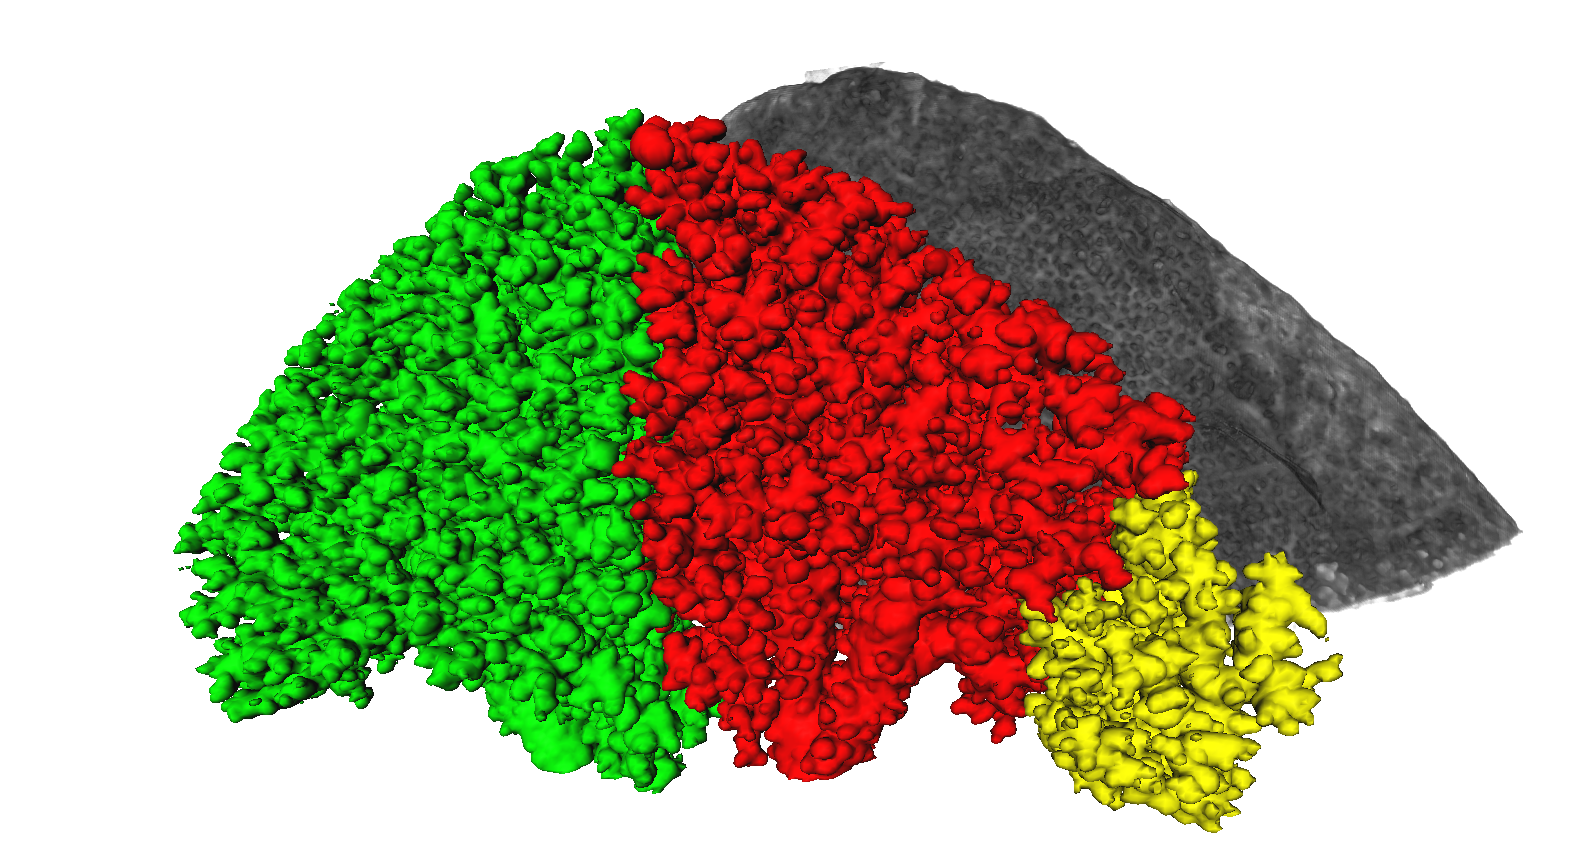
\includegraphics[width=\imagewidth]{img/comparisonBvsT/R108C21_overview_B}};%
				% 1237px = 4.0138mm > 100px = 324um > 154px = 500um
				\draw[|-|,thick] (160,659) -- (1393,764) node [sloped,midway,above] {\SI{4.0138}{\milli\meter}};%
				\draw[|-|,thick] (\x,\y) -- (\x+154,\y) node [right] {\SI{500}{\micro\meter}};%
			\end{tikzpicture}%
		&%
			\pgfmathsetlength{\imagewidth}{\imsize}%
			\pgfmathsetlength{\imagescale}{\imagewidth/1594}%
			\def\x{225}%
			\def\y{825}%
			\label{subfig:BvsToverviewT}%
			\begin{tikzpicture}[x=\imagescale,y=-\imagescale]%
				\node[anchor=north west,inner sep=0pt,outer sep=0pt] at (0,0)%
					{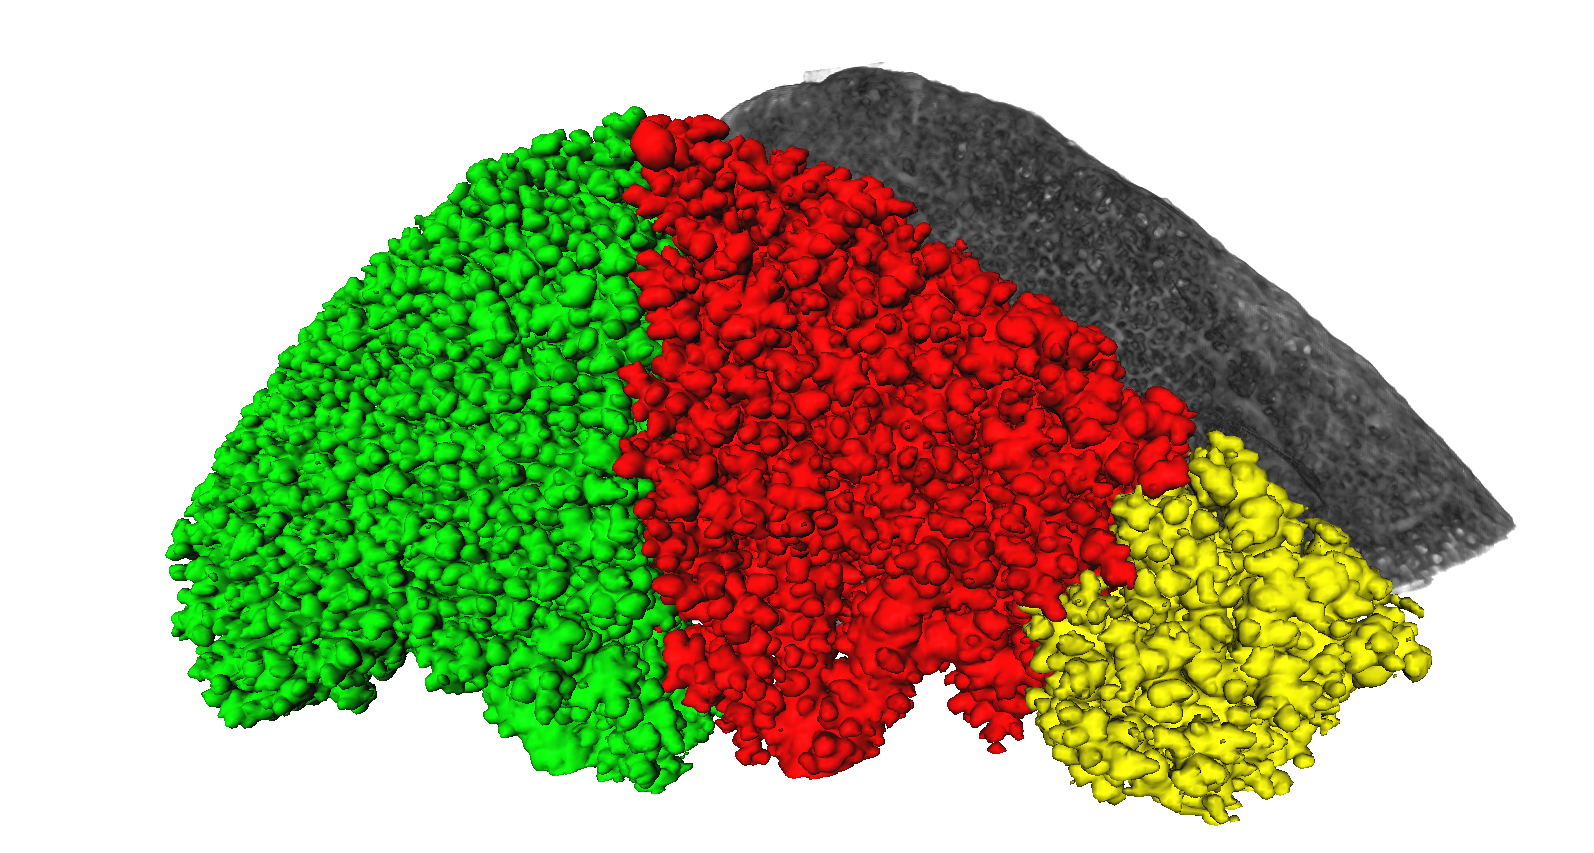
\includegraphics[width=\imagewidth]{img/comparisonBvsT/R108C21_overview_T}};%
				% 1329px = 4.0138mm > 100px = 302um > 166px = 500um
				\draw[|-|,thick] (154,667) -- (1477,793) node [sloped,midway,above] {\SI{4.0138}{\milli\meter}};%
				\draw[|-|,thick] (\x,\y) -- (\x+166,\y) node [right] {\SI{500}{\micro\meter}};%
			\end{tikzpicture}%
		\\%
		a) Overview Protocol B & b) Overview Protocol T%
		\\%
		\pgfmathsetlength{\imagewidth}{\imsize}%
		\pgfmathsetlength{\imagescale}{\imagewidth/1594}%
		\def\x{225}%
		\def\y{675}%
			\label{subfig:BvsTsegmentB}%
			\begin{tikzpicture}[x=\imagescale,y=-\imagescale]%
				\node[anchor=north west,inner sep=0pt,outer sep=0pt] at (0,0)%
					{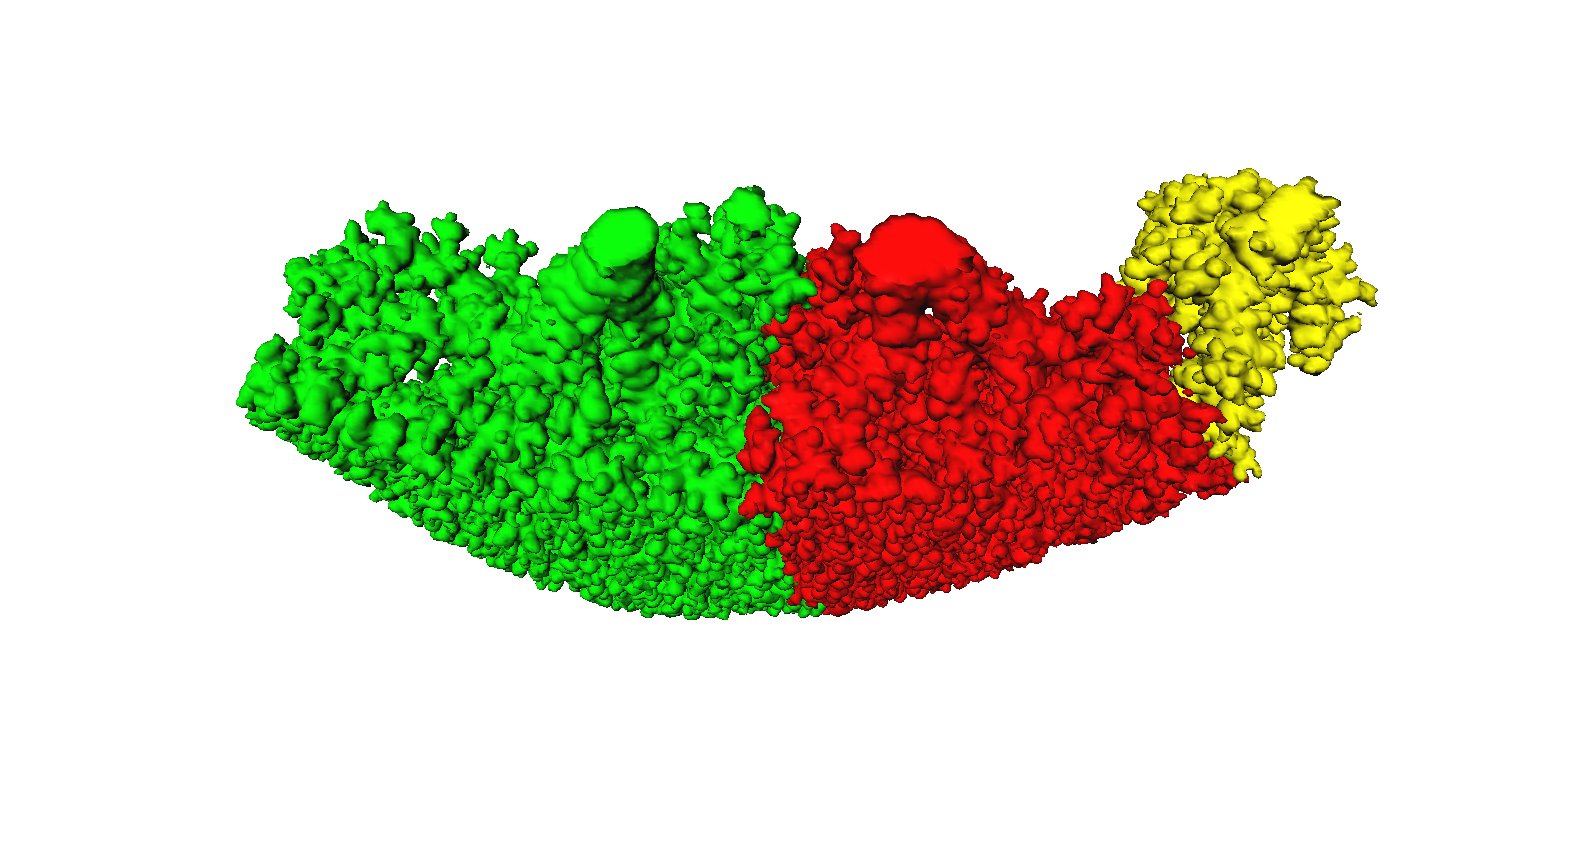
\includegraphics[width=\imagewidth]{img/comparisonBvsT/R108C21_underside_iso_B}};%
				% 1269px = 4.0138mm > 100px = 316um > 158px = 500um
				\draw[|-|,thick] (171,265) -- (1439,270) node [sloped,midway,above] {\SI{4.0138}{\milli\meter}};%
				\draw[|-|,thick] (\x,\y) -- (\x+158,\y) node [right] {\SI{500}{\micro\meter}};%
			\end{tikzpicture}%
		&%
			\pgfmathsetlength{\imagewidth}{\imsize}%
			\pgfmathsetlength{\imagescale}{\imagewidth/1594}%
			\def\x{225}%
			\def\y{675}%
			\label{subfig:BvsTsegmentT}%
			\begin{tikzpicture}[x=\imagescale,y=-\imagescale]%
				\node[anchor=north west,inner sep=0pt,outer sep=0pt] at (0,0)%
				{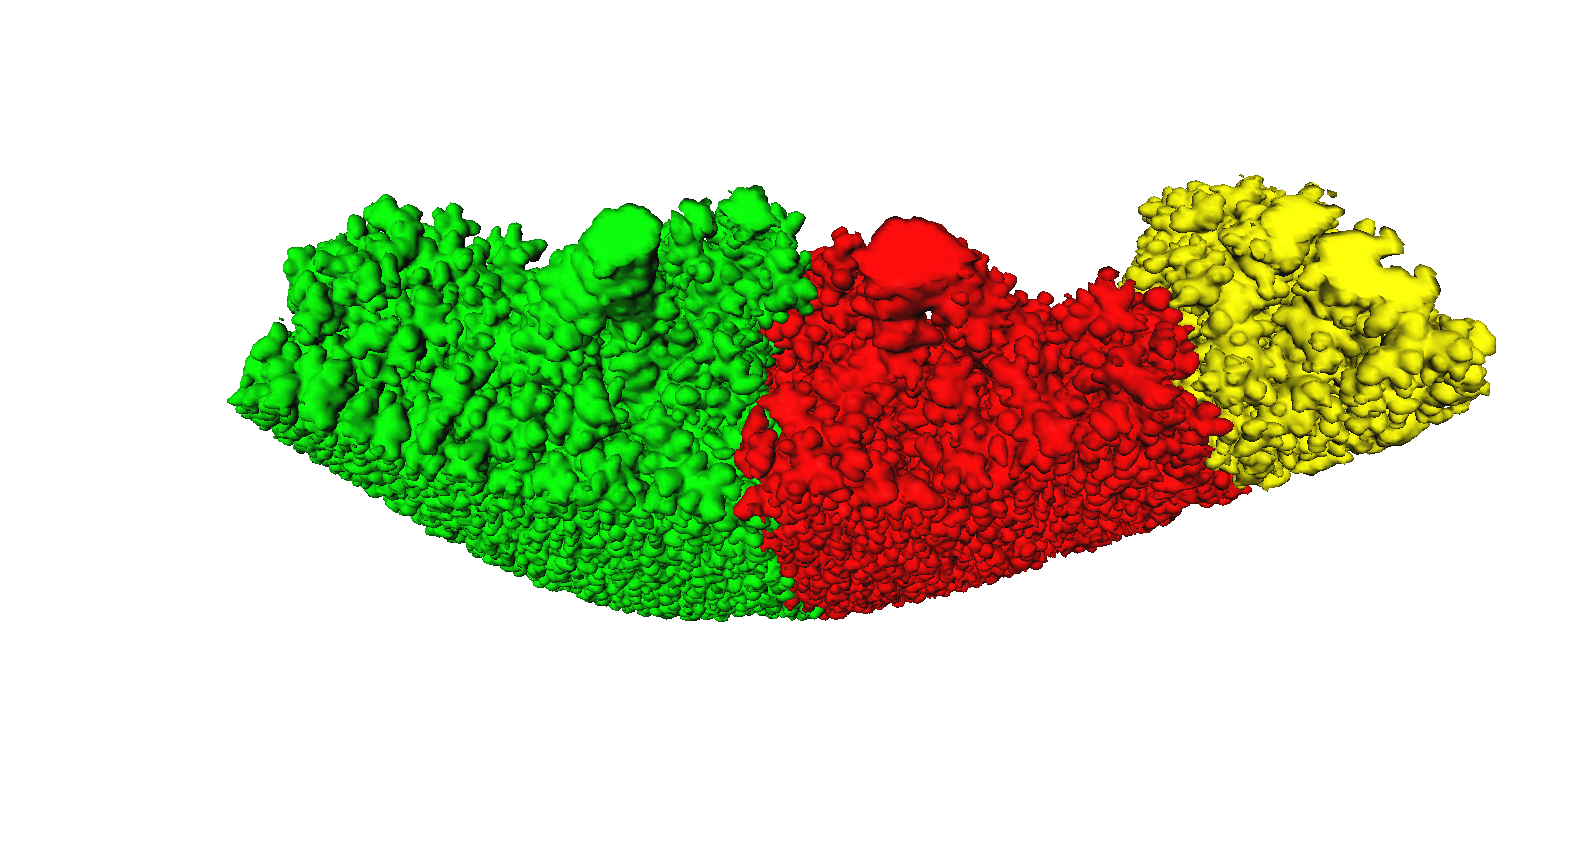
\includegraphics[width=\imagewidth]{img/comparisonBvsT/R108C21_underside_iso_T}};%
				% 1269px = 4.0138mm > 100px = 316um > 158px = 500um
				\draw[|-|,thick] (171,265) -- (1439,270) node [sloped,midway,above] {\SI{4.0138}{\milli\meter}};%
				\draw[|-|,thick] (\x,\y) -- (\x+158,\y) node [right] {\SI{500}{\micro\meter}};%
			\end{tikzpicture}%
		\\%
			c) Segmented airways for protocol B & d) Segmented airways for protocol T%
		\\%&
			\pgfmathsetlength{\imagewidth}{\imsize}%
			\pgfmathsetlength{\imagescale}{\imagewidth/2712}% pixel width of imagefile used		
			\def\x{383}%
			\def\y{150}%
			\label{subfig:BvsTsliceB}%
			\begin{tikzpicture}[x=\imagescale,y=-\imagescale]%
			  \node[anchor=north west,inner sep=0pt,outer sep=0pt] at (0,0)%
			     {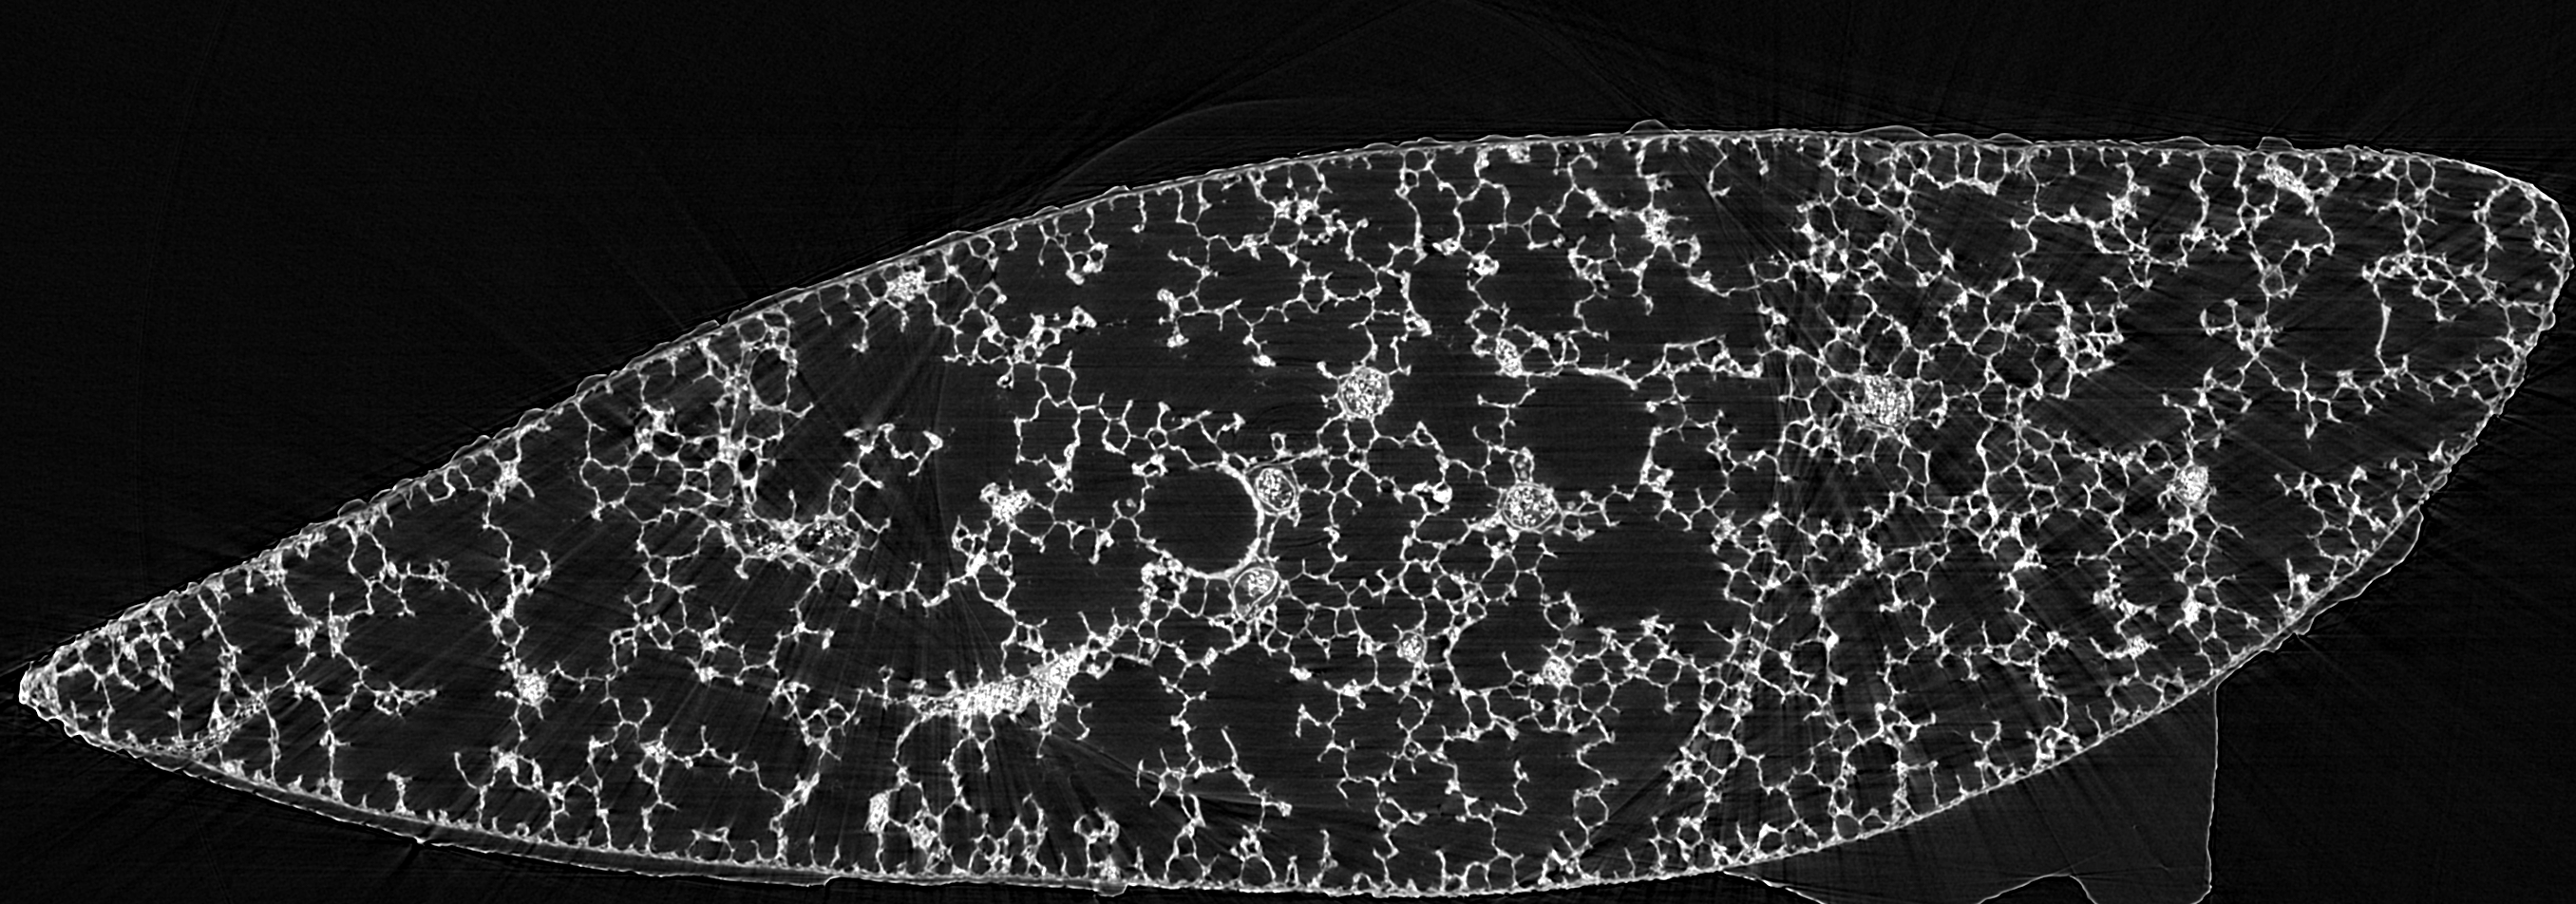
\includegraphics[width=\imagewidth]{img/protocols/R108C21Cb_mrg1024}};%
				% 2710px = 4.0138mm > 100px = 148um > 338px = 500um
				\draw[|-|,color=white,thick] (2712,742) -- (1,742) node [midway,above] {\SI{4.0138}{\milli\meter}};%
				\draw[|-|,color=white,thick] (\x,\y) -- (\x+338,\y) node [right] {\SI{500}{\micro\meter}};%
			\end{tikzpicture}%
		&%
			\pgfmathsetlength{\imagewidth}{\imsize}%
			\pgfmathsetlength{\imagescale}{\imagewidth/2712}% pixel width of imagefile used		
			\def\x{383}%
			\def\y{150}%
			\label{subfig:BvsTsliceT}%
			\begin{tikzpicture}[x=\imagescale,y=-\imagescale]
			  \node[anchor=north west,inner sep=0pt,outer sep=0pt] at (0,0)
			     {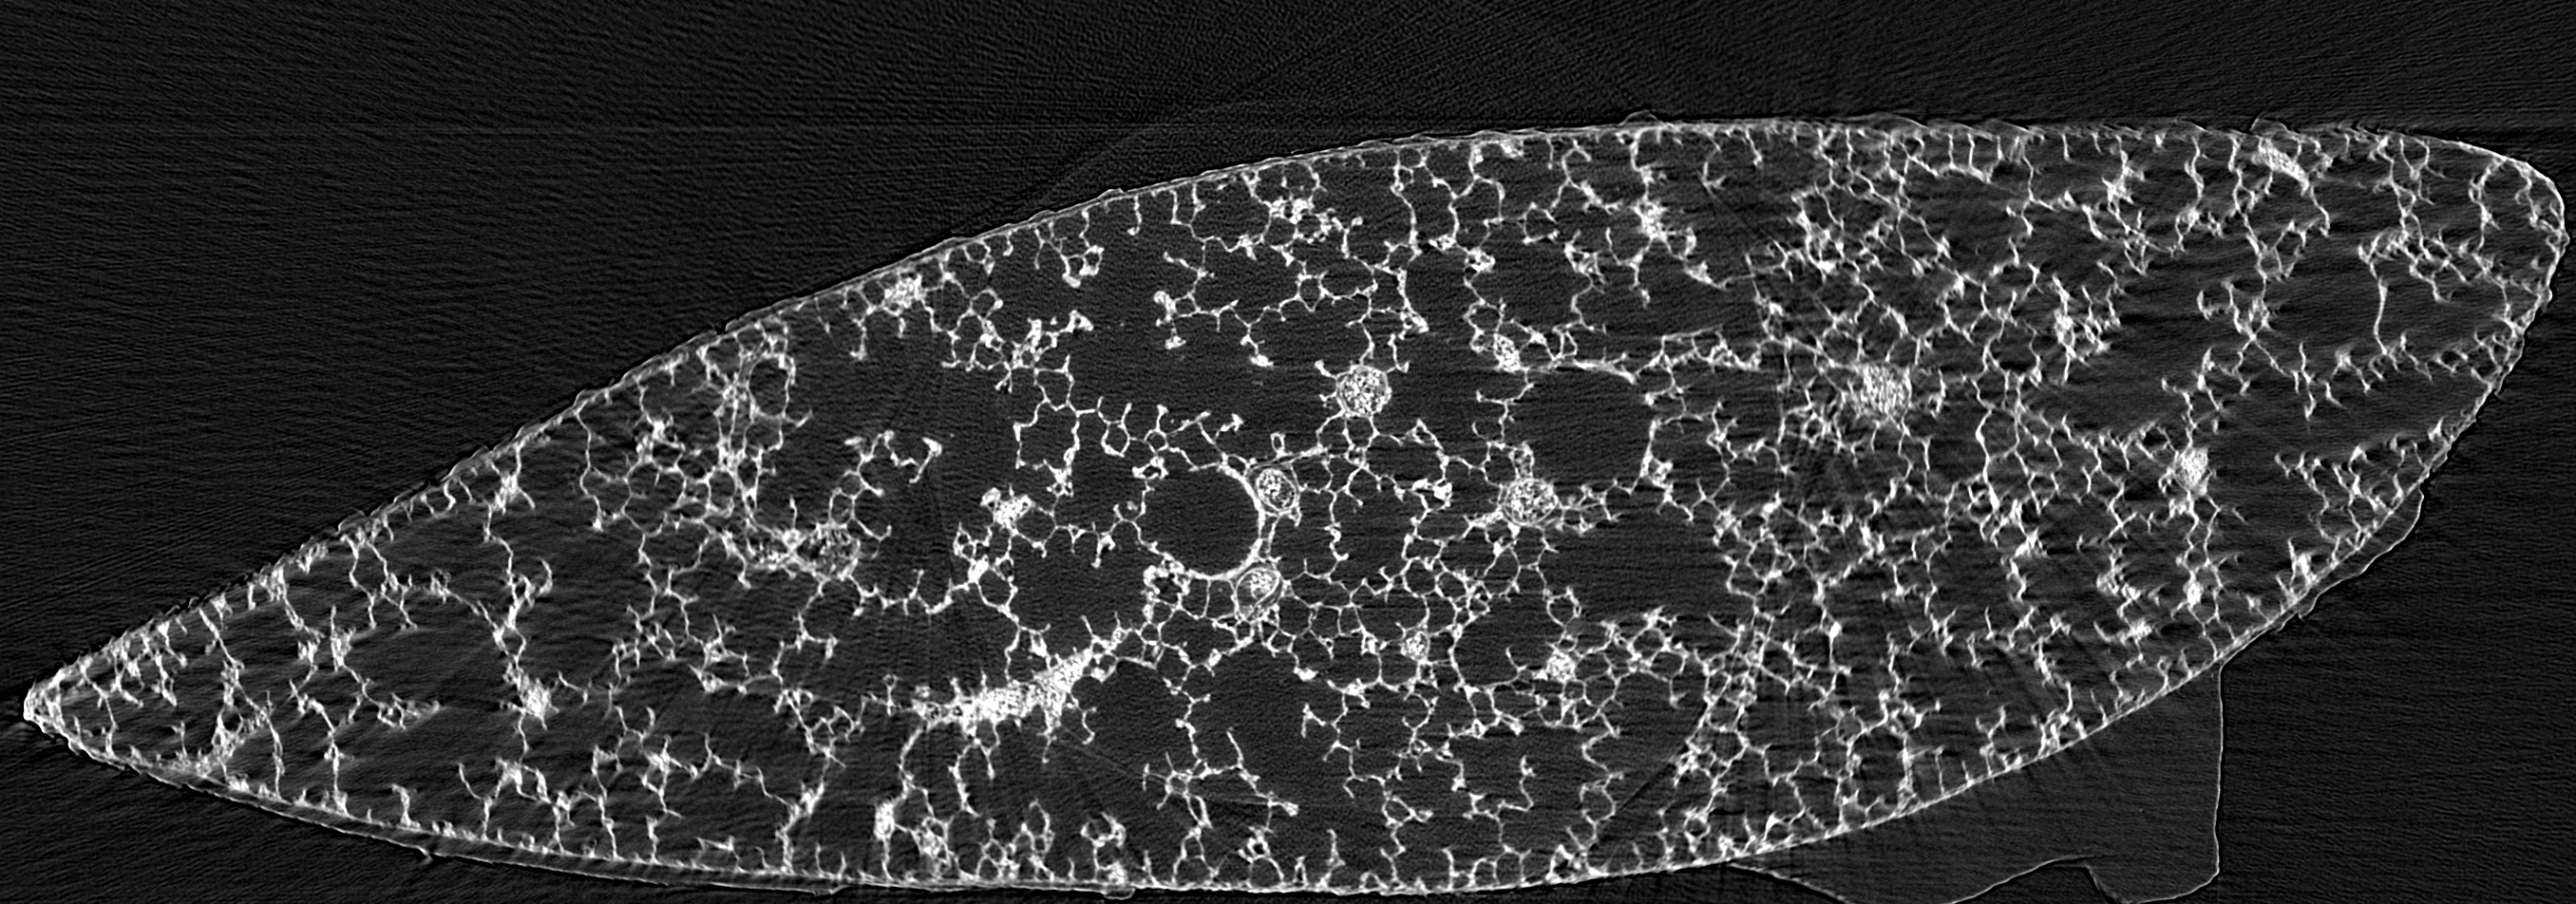
\includegraphics[width=\imagewidth]{img/protocols/R108C21Ct_mrg1024}};
				% 2712px = 4.0138mm > 100px = 148um > 338px = 500um
				\draw[|-|,color=white,thick] (0,760) -- (2712,758) node [midway,above] {\SI{4.0138}{\milli\meter}};
				\draw[|-|,color=white,thick] (\x,\y) -- (\x+338,\y) node [right] {\SI{500}{\micro\meter}};
			\end{tikzpicture}%
		\\%
			e) Slice 1024 of dataset for protocol B, reconstructed from 5244 merged projections.%
		&%			
			f) Slice 1024 of dataset for protocol T, reconstructed from 874 merged projections.%
	\end{tabular}%
	\label{fig:BvsT}%
\end{figure}%
%\twocolumn
%%% iucr %%%
%%% normal figures %%%
%%\begin{figure*}[htp]
%%	\renewcommand{\imsize}{.5\linewidth}
%%	\centering
%%	\pgfmathsetlength{\imagewidth}{\imsize}%
%%	\pgfmathsetlength{\imagescale}{\imagewidth/1594}%
%%	\def\x{225}%
%%	\def\y{825}%
%%	\subfloat[Overview Protocol B]{%
%%		\label{subfig:BvsToverviewB}%
%%	    \begin{tikzpicture}[x=\imagescale,y=-\imagescale]
%%			\node[anchor=north west,inner sep=0pt,outer sep=0pt] at (0,0)
%%				{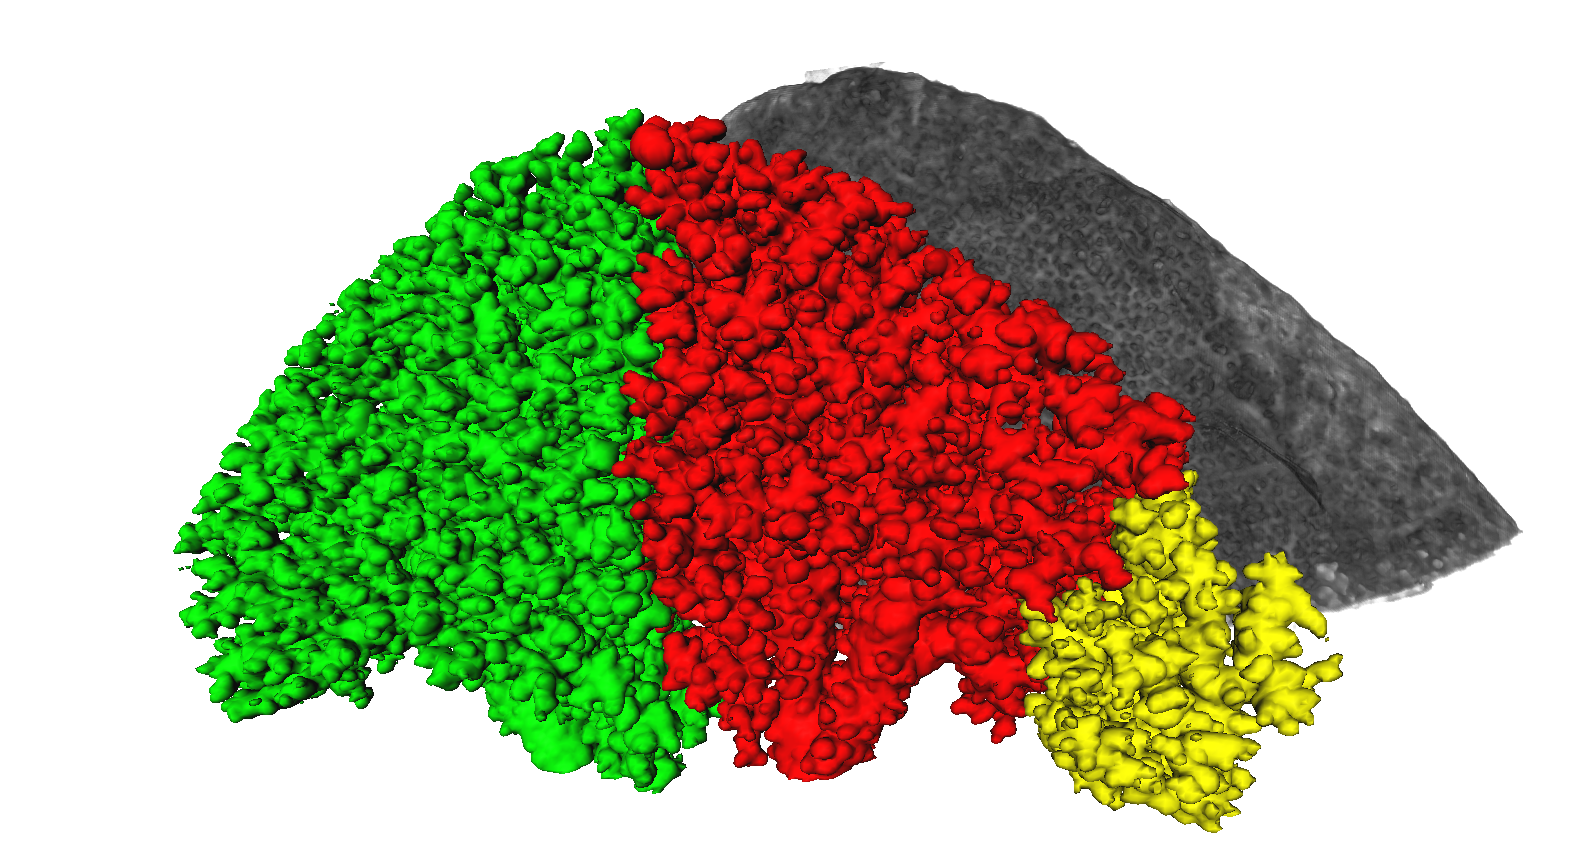
\includegraphics[width=\imagewidth]{img/comparisonBvsT/R108C21_overview_B}};
%%			% 1237px = 4.0138mm > 100px = 324um > 154px = 500um
%%			\draw[|-|,thick] (160,659) -- (1393,764) node [sloped,midway,above] {\SI{4.0138}{\milli\meter}};
%%			\draw[|-|,thick] (\x,\y) -- (\x+154,\y) node [right] {\SI{500}{\micro\meter}};
%%		\end{tikzpicture}%
%%		}%
%%	\subfloat[Overview Protocol T]{%
%%		\label{subfig:BvsToverviewT}%
%%		\begin{tikzpicture}[x=\imagescale,y=-\imagescale]
%%			\node[anchor=north west,inner sep=0pt,outer sep=0pt] at (0,0)
%%				{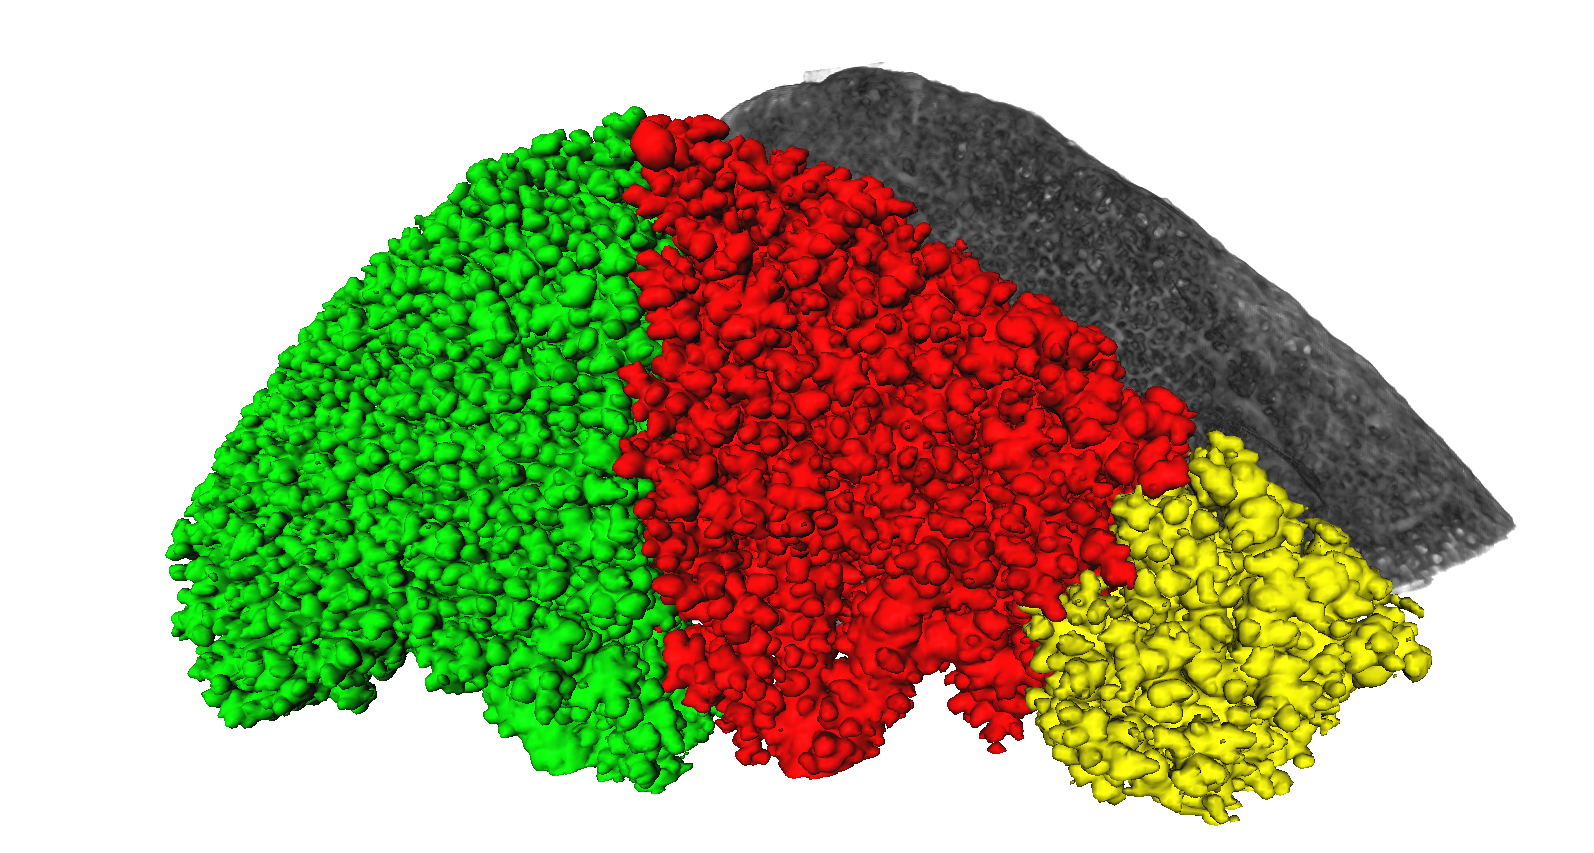
\includegraphics[width=\imagewidth]{img/comparisonBvsT/R108C21_overview_T}};
%%			% 1329px = 4.0138mm > 100px = 302um > 166px = 500um
%%			\draw[|-|,thick] (154,667) -- (1477,793) node [sloped,midway,above] {\SI{4.0138}{\milli\meter}};
%%			\draw[|-|,thick] (\x,\y) -- (\x+166,\y) node [right] {\SI{500}{\micro\meter}};
%%		\end{tikzpicture}%
%%		}\\%
%%	\def\x{225}%
%%	\def\y{675}%
%%	\subfloat[Segmented airways for protocol B]{%
%%		\label{subfig:BvsTsegmentB}%
%%		\begin{tikzpicture}[x=\imagescale,y=-\imagescale]
%%			\node[anchor=north west,inner sep=0pt,outer sep=0pt] at (0,0)
%%				{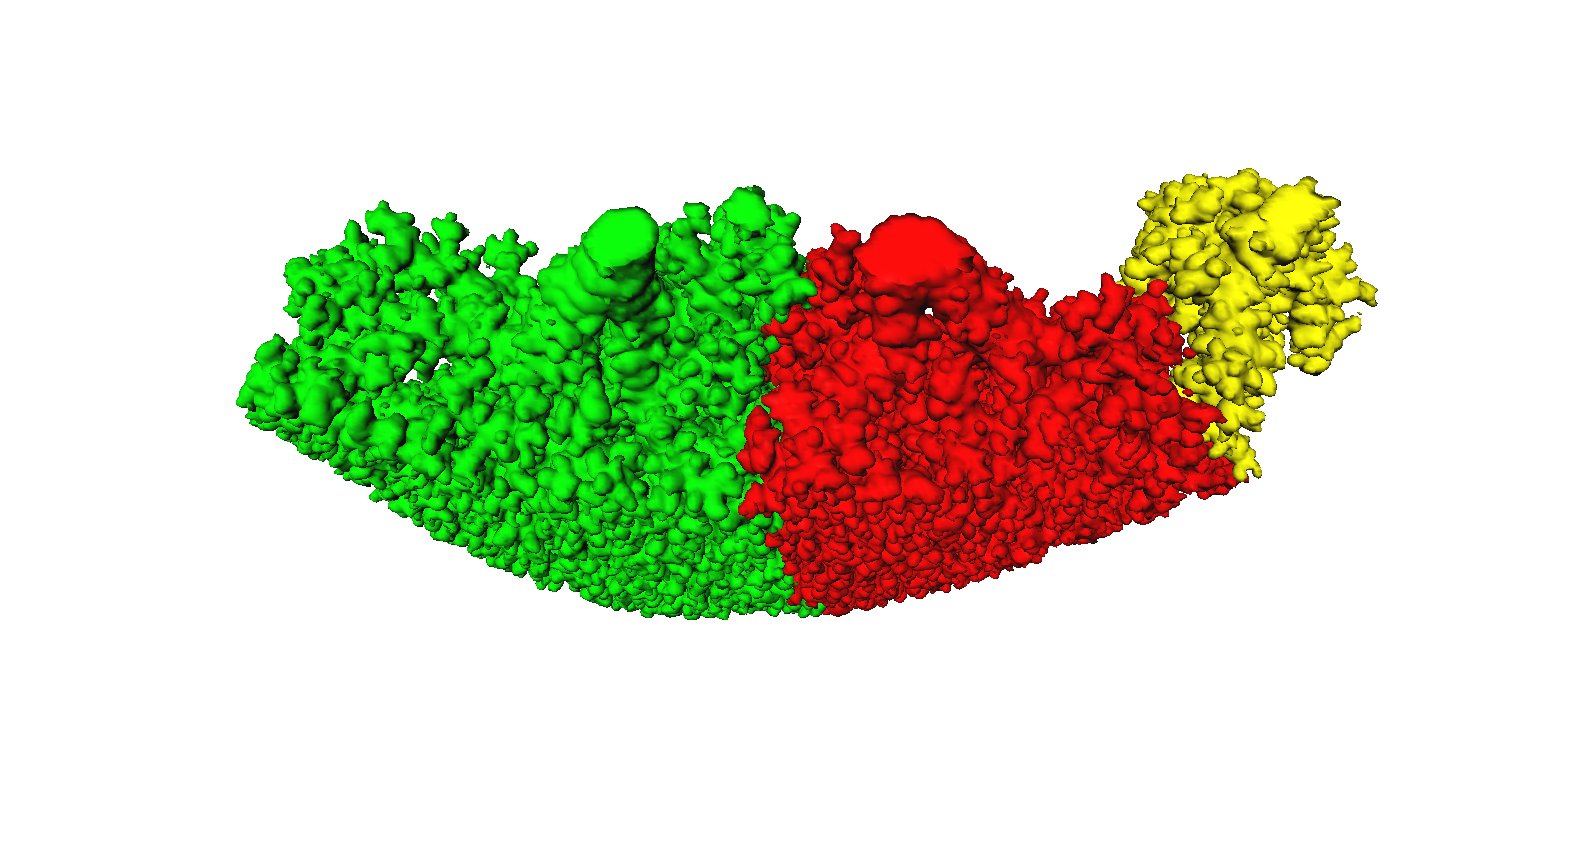
\includegraphics[width=\imagewidth]{img/comparisonBvsT/R108C21_underside_iso_B}};
%%			% 1269px = 4.0138mm > 100px = 316um > 158px = 500um
%%			\draw[|-|,thick] (171,265) -- (1439,270) node [sloped,midway,above] {\SI{4.0138}{\milli\meter}};
%%			\draw[|-|,thick] (\x,\y) -- (\x+158,\y) node [right] {\SI{500}{\micro\meter}};
%%		\end{tikzpicture}%
%%	}%
%%	\subfloat[Segmented airways for protocol T]{%
%%		\label{subfig:BvsTsegmentT}%
%%		\begin{tikzpicture}[x=\imagescale,y=-\imagescale]
%%			\node[anchor=north west,inner sep=0pt,outer sep=0pt] at (0,0)
%%			{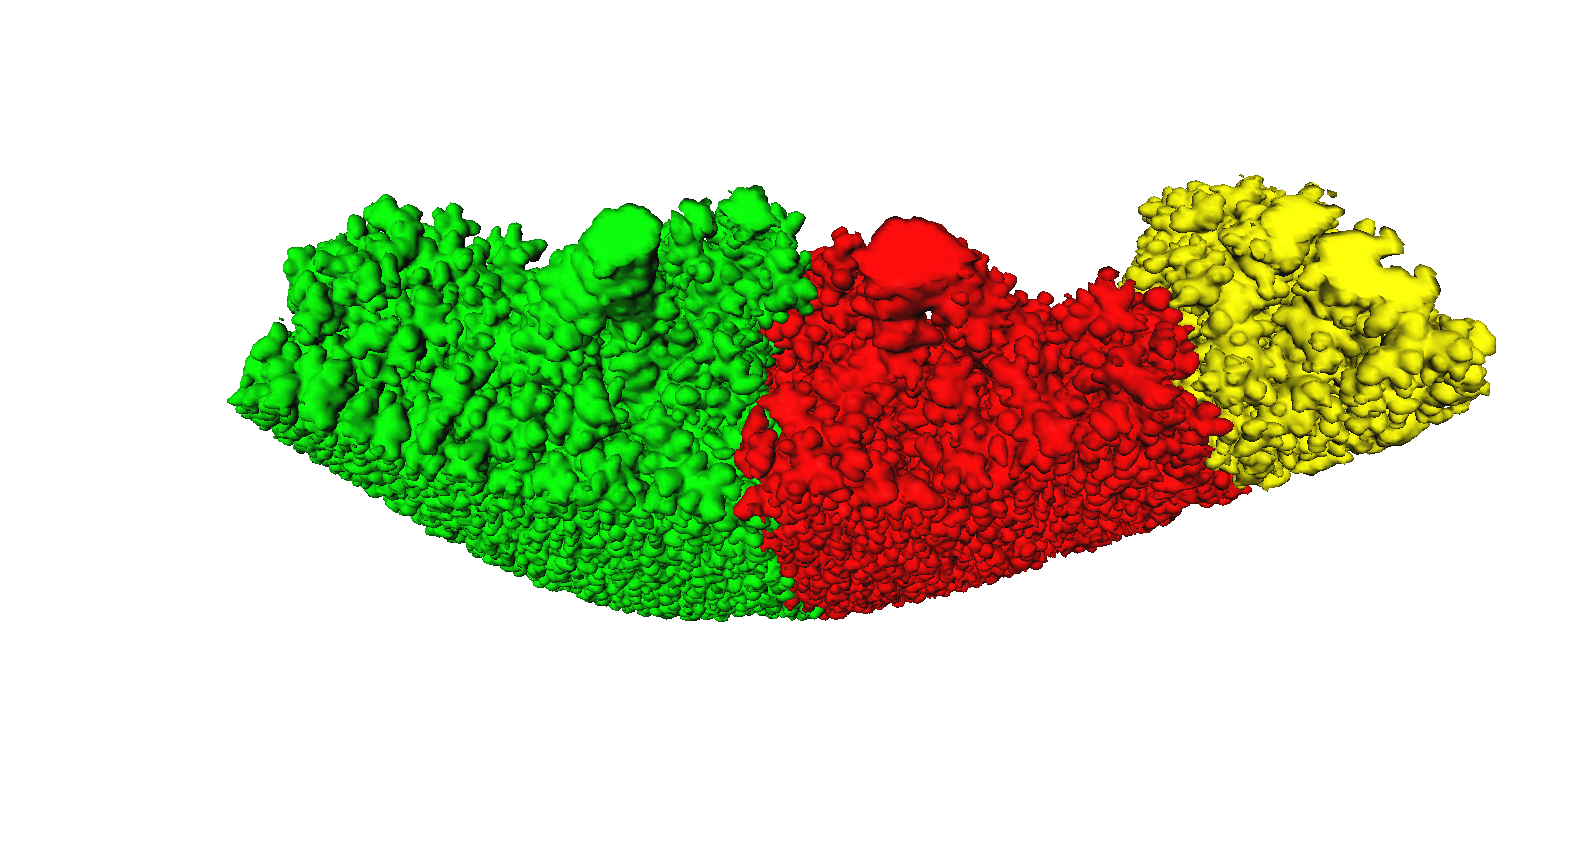
\includegraphics[width=\imagewidth]{img/comparisonBvsT/R108C21_underside_iso_T}};
%%			% 1269px = 4.0138mm > 100px = 316um > 158px = 500um
%%			\draw[|-|,thick] (171,265) -- (1439,270) node [sloped,midway,above] {\SI{4.0138}{\milli\meter}};
%%			\draw[|-|,thick] (\x,\y) -- (\x+158,\y) node [right] {\SI{500}{\micro\meter}};
%%		\end{tikzpicture}%
%%		}\\%
%%	\pgfmathsetlength{\imagescale}{\imagewidth/2712}% pixel width of imagefile used		
%%	\def\x{383}%
%%	\def\y{150}%
%%	\subfloat[Slice 1024 of dataset for protocol B, reconstructed from 5244 merged projections.]{%
%%		\label{subfig:BvsTsliceB}%
%%		\begin{tikzpicture}[x=\imagescale,y=-\imagescale]
%%		  \node[anchor=north west,inner sep=0pt,outer sep=0pt] at (0,0)
%%		     {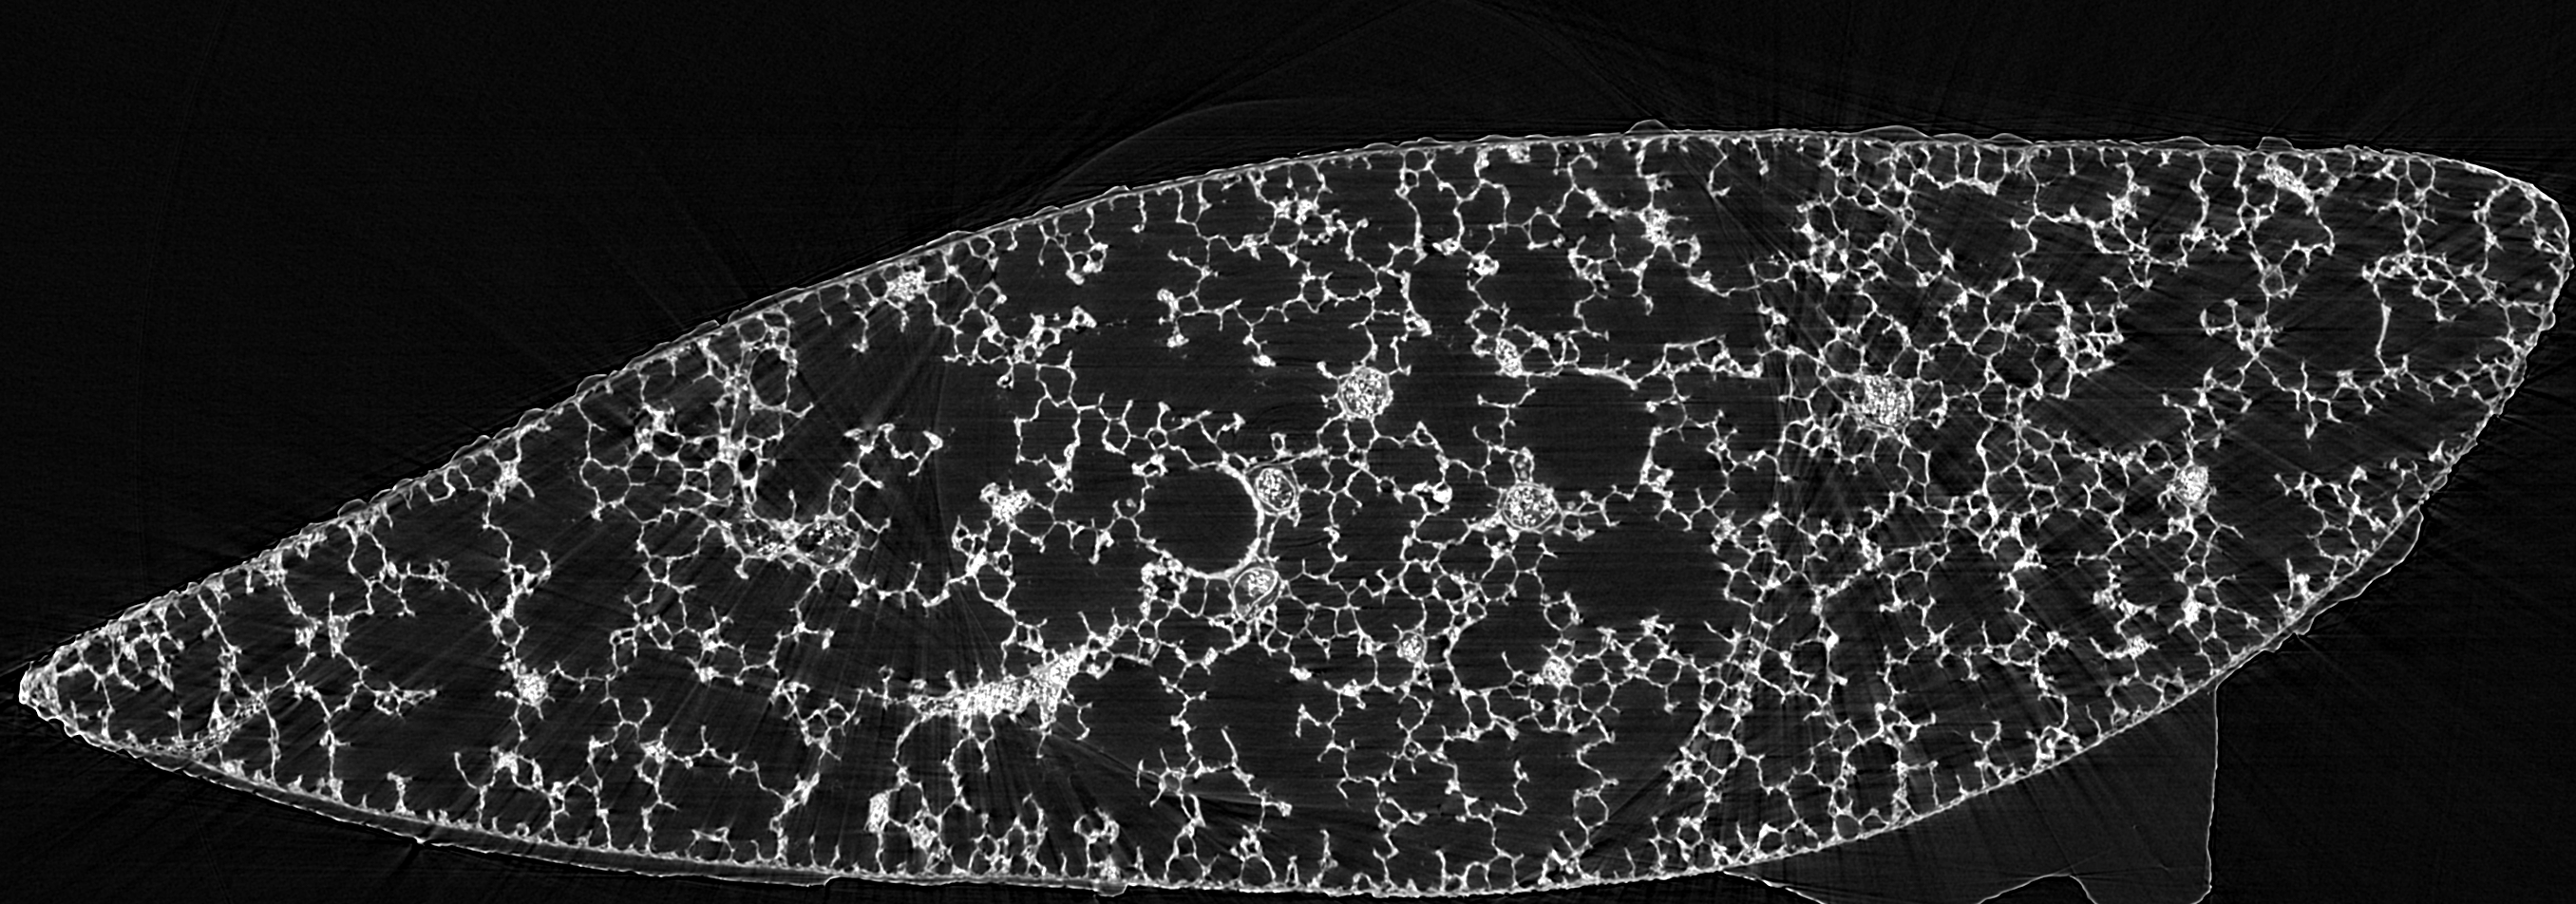
\includegraphics[width=\imagewidth]{img/protocols/R108C21Cb_mrg1024}};
%%			% 2710px = 4.0138mm > 100px = 148um > 338px = 500um
%%			\draw[|-|,color=white,thick] (2712,742) -- (1,742) node [midway,above] {\SI{4.0138}{\milli\meter}};
%%			\draw[|-|,color=white,thick] (\x,\y) -- (\x+338,\y) node [right] {\SI{500}{\micro\meter}};
%%		\end{tikzpicture}%
%%		}%
%%	\subfloat[Slice 1024 of dataset for protocol T, reconstructed from 874 merged projections.]{%
%%		\label{subfig:BvsTsliceT}%
%%		\begin{tikzpicture}[x=\imagescale,y=-\imagescale]
%%		  \node[anchor=north west,inner sep=0pt,outer sep=0pt] at (0,0)
%%		     {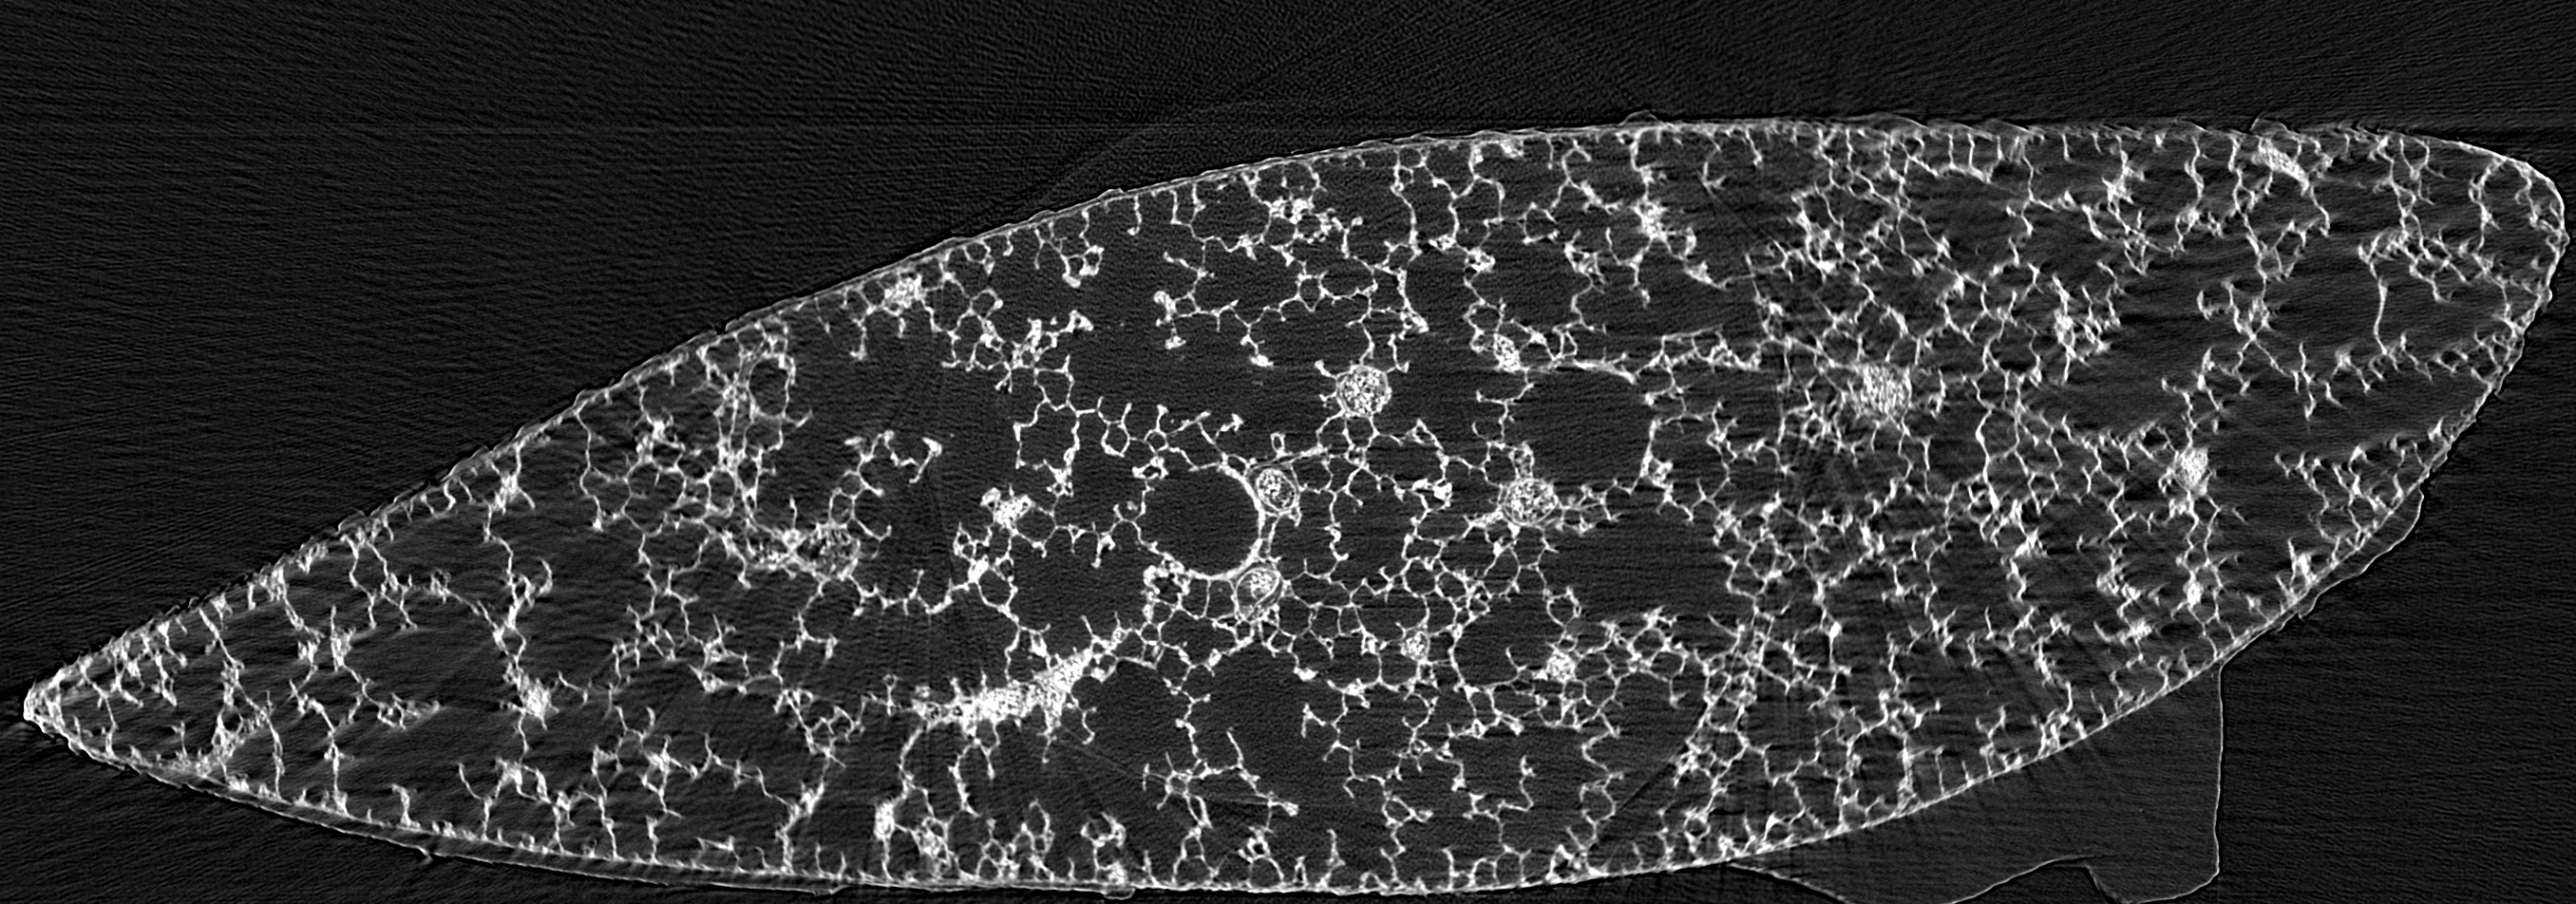
\includegraphics[width=\imagewidth]{img/protocols/R108C21Ct_mrg1024}};
%%			% 2712px = 4.0138mm > 100px = 148um > 338px = 500um
%%			\draw[|-|,color=white,thick] (0,760) -- (2712,758) node [midway,above] {\SI{4.0138}{\milli\meter}};
%%			\draw[|-|,color=white,thick] (\x,\y) -- (\x+338,\y) node [right] {\SI{500}{\micro\meter}};
%%		\end{tikzpicture}%
%%		}\\
%%	\caption{Comparison of protocols B and T. Top row: overview. Center row: view of the isosurfaces of the segmented airways. Bottom row: Slices}%
%%	\label{fig:BvsT}%
%%\end{figure*}
%%% normal figures %%%

The protocols shown in figure~\ref{fig:BvsT} are the two extremes of the 19 obtained protocols  in terms of scanning time. Protocol B is the gold standard, obtained with in total 15732 projections recorded in 65 minutes. Protocol T has been obtained in just \SI{13.75}{\percent} of the scanning time, with in total 2185 projections recorded in 12 minutes (\SI{13.75}{\percent} of 65 minutes would be 9 minutes, the 3 minute difference arises through the movement of the sample which cannot be reduced with the recording of less projections). Hence, the dataset from protocol B has been reconstructed from 5244 merged projection images, the dataset from protocol T has been reconstructed using only 874 merged slices. Albeit we have scanned protocol T while violating the sampling theorem, both samples still appear to be nearly identical in the three dimensional visualization. Except for small differences at the most lateral parts of the sample (yellow segment) the segmented airways appear to identical, even if the scanning time of protocol T has been reduced to \SI{13.75}{\percent} of the scanning time of protocol B.

Only when taking a closer look to a crop of the three dimensional dataset---as shown in figure~\ref{fig:BvsT2}---the artifacts introduced through the great reduction in scanning time become apparent. The blue cube inside the green airway segments in figures~\ref{subfig:DetailOverviewB} and \ref{subfig:DetailOverviewT} are shown as isosurface visualizations of the lung tissue (which exactly corresponds to the negative of the extracted airway segment) in figures~\ref{subfig:DetailROIB} and \ref{subfig:DetailROIT}.

Both those regions of interest are a cube with a side length of \SI{190}{\micro\meter} and only on this scale the difference between the two protocols B and T is visible. We see that the isosurface of the ROI of protocol T shown in figure~\ref{subfig:DetailROIT} appears rougher than the isosurface of protocol B shown in figure~\ref{subfig:DetailROIB}. This roughness is introduced through the wave-like artifacts visible in the original slice of the dataset of protocol T shown in figure~\ref{subfig:BvsTsliceT}%
\todo{do we need to show a close-up of the background to be able to see it?}%
which arise through the breaching of the sampling theorem, since we have only acquired 874 projections for the outer scan (2185 projections in total for protocol T) instead of the 5139 projections ($(3072+200)\frac{\pi}{2}$) that would be necessary to satisfy the sampling theorem. But even with this strong undersampling a segmentation, three dimensional reconstruction and visualization of the sample is still possible. Thus, if the user desired to gain a quick overview over his sample, e.g.\ to quickly assess the integrity of multiple samples over a short time, such a time-saving protocol could be used.

%%% iucr %%%
%\onecolumn%
\begin{figure}%
	\centering%
	\caption{Comparison of three-dimensional visualizations of protocols B and T. Top: Three independent airway segments (green, red, yellow) have been extracted using a region growing algorithm. A cubical region of interest (ROI, blue) with a side length of 128 pixels (corresponding to \SI{190}{\micro\meter}) is marked inside the leftmost segment for both protocols. Bottom: Detailed view of isosurfaces of the lung tissue inside the ROIs shown above. Note the artifacts in the reconstructions for protocol T in subfigure d).}%
	\begin{tabular}{cc}%
		\renewcommand{\imsize}{.5\linewidth}%
		\pgfmathsetlength{\imagewidth}{\imsize}%
		\pgfmathsetlength{\imagescale}{\imagewidth/1397}%
		\def\x{100}%
		\def\y{150}%
		\begin{tikzpicture}[x=\imagescale,y=-\imagescale]%
			\node[anchor=north west,inner sep=0pt,outer sep=0pt] at (0,0)%
				{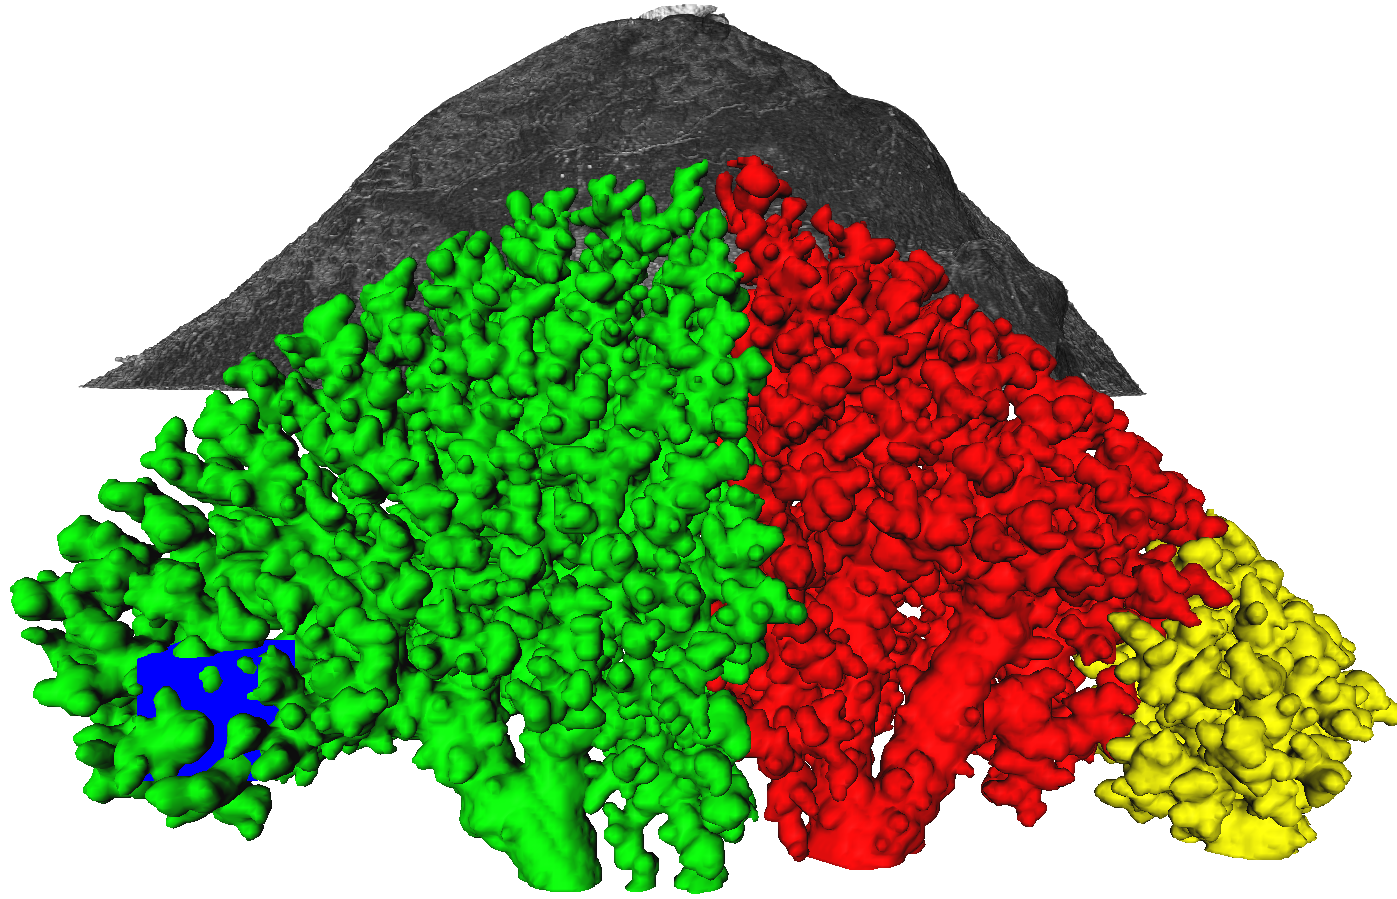
\includegraphics[width=\imagewidth]{img/comparisonBvsT/overview-b}};%
			% 1391px = 4.0138mm > 100px = 288um > 173px = 500um
			\draw[|-|,thick] (6,774) -- (1395,839) node [sloped,midway,above] {\SI{4.0138}{\milli\meter}};%
			\draw[|-|,thick] (\x,\y) -- (\x+173,\y) node [midway,above] {\SI{500}{\micro\meter}};%
		\end{tikzpicture}%
		\label{subfig:DetailOverviewB}%
	&%
		\renewcommand{\imsize}{.5\linewidth}%
		\pgfmathsetlength{\imagewidth}{\imsize}%
		\pgfmathsetlength{\imagescale}{\imagewidth/1397}%
		\def\x{100}%
		\def\y{150}%
		\begin{tikzpicture}[x=\imagescale,y=-\imagescale]%
			\node[anchor=north west,inner sep=0pt,outer sep=0pt] at (0,0)%
				{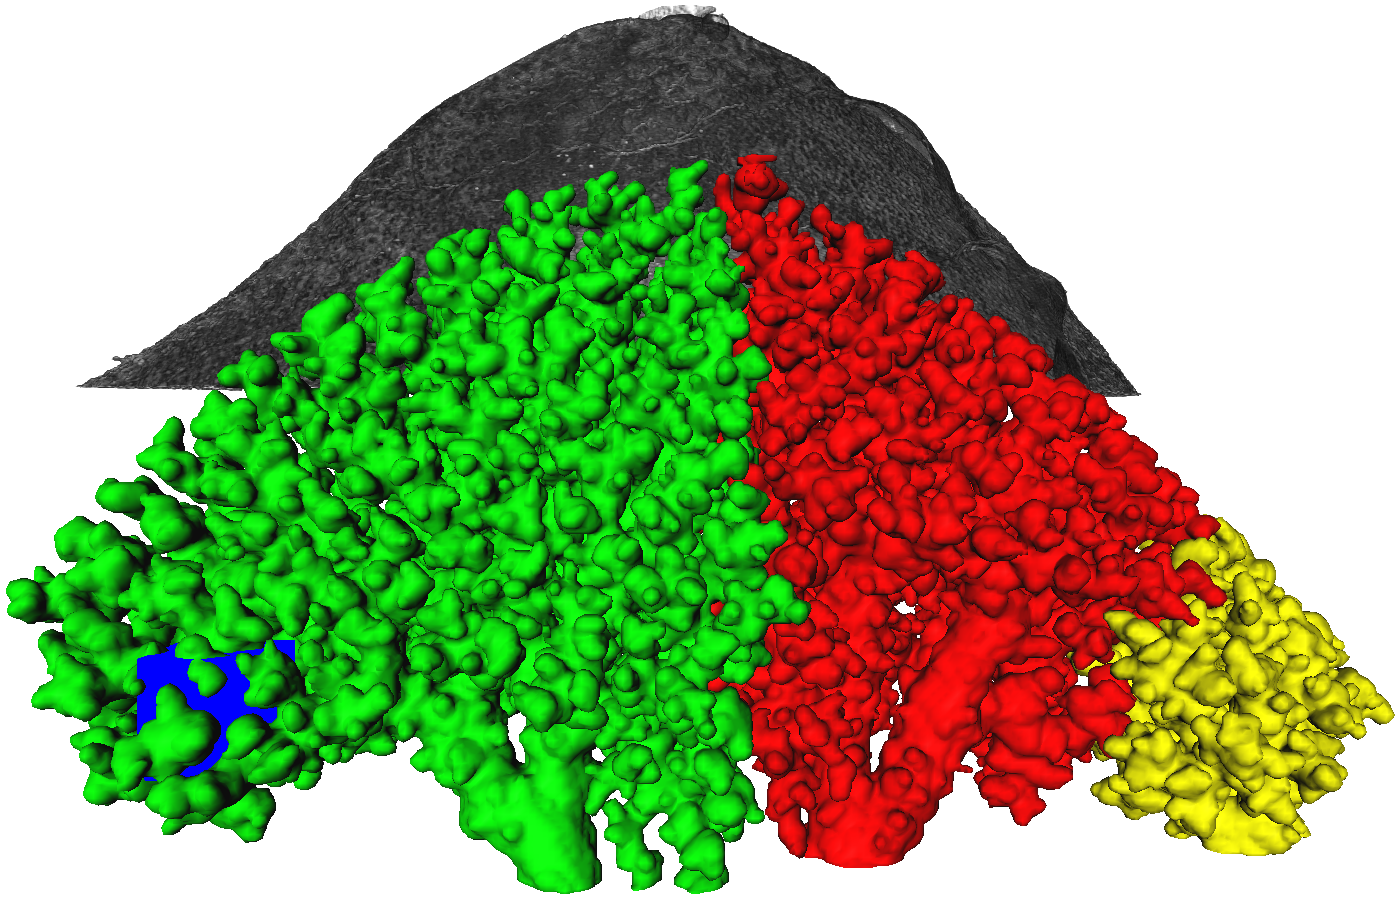
\includegraphics[width=\imagewidth]{img/comparisonBvsT/overview-t}};%
			% 1391px = 4.0138mm > 100px = 288um > 173px = 500um
			\draw[|-|,thick] (6,774) -- (1395,839) node [sloped,midway,above] {\SI{4.0138}{\milli\meter}};%
			\draw[|-|,thick] (\x,\y) -- (\x+173,\y) node [midway,above] {\SI{500}{\micro\meter}};%
		\end{tikzpicture}%
		\label{subfig:DetailOverviewT}%
	\\%
		a) Overview of protocol B%
	&%
		b) Overview of protocol T%
	\\%
		\renewcommand{\imsize}{.5\linewidth}%
		\pgfmathsetlength{\imagewidth}{\imsize}%
		\pgfmathsetlength{\imagescale}{\imagewidth/806}%
		\def\x{345}%
		\def\y{780}%
		\label{subfig:DetailROIB}%
		\begin{tikzpicture}[x=\imagescale,y=-\imagescale]%
			\node[anchor=north west,inner sep=0pt,outer sep=0pt] at (0,0)%
				{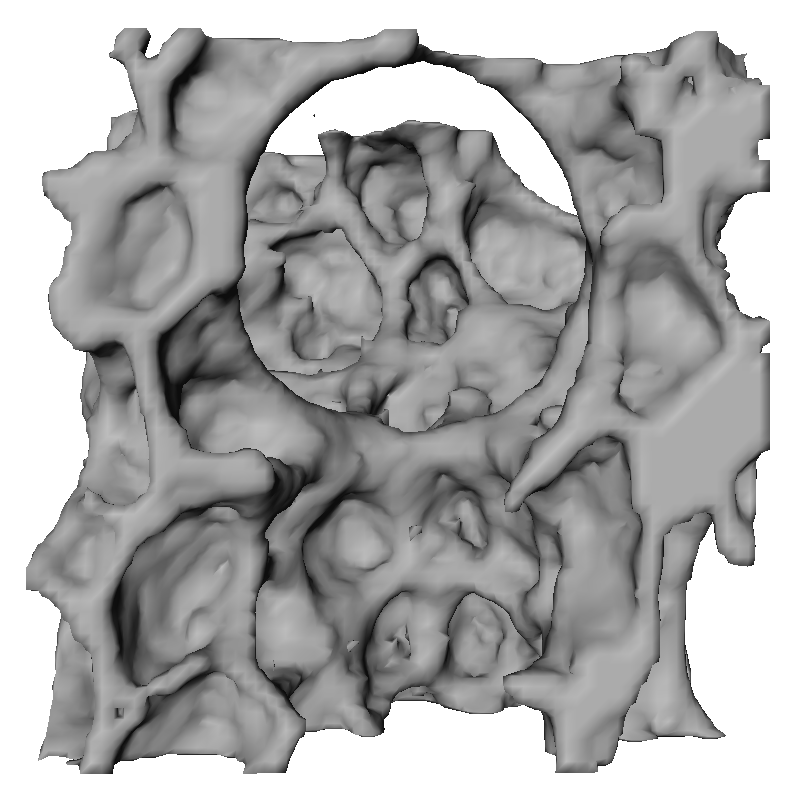
\includegraphics[width=\imagewidth]{img/comparisonBvsT/roi-b-nomedian}};%
			% 746px = 0.18944mm > 100px = 25um > 196.9px = 50um
			\draw[|-|,thick] (27,270) -- (773,272) node [sloped,midway,above] {\SI{189.44}{\micro\meter}};%
			\draw[|-|,thick] (\x,\y) -- (\x+196.9,\y) node [midway,above] {\SI{50}{\micro\meter}};%
		\end{tikzpicture}%
	&%
		\renewcommand{\imsize}{.5\linewidth}%
		\pgfmathsetlength{\imagewidth}{\imsize}%
		\pgfmathsetlength{\imagescale}{\imagewidth/806}%
		\def\x{345}%
		\def\y{780}%
		\label{subfig:DetailROIT}%
		\begin{tikzpicture}[x=\imagescale,y=-\imagescale]%
			\node[anchor=north west,inner sep=0pt,outer sep=0pt] at (0,0)%
				{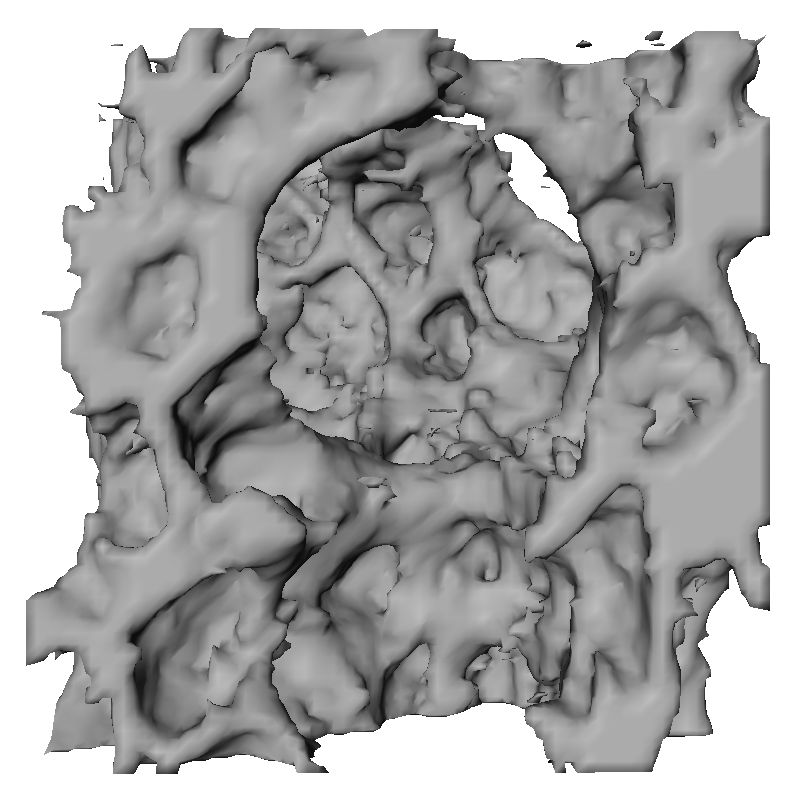
\includegraphics[width=\imagewidth]{img/comparisonBvsT/roi-t-nomedian}};%
			% 744px = 0.18944mm > 100px = 25um > 196.5px = 50um
			\draw[|-|,thick] (27,311) -- (771,311) node [sloped,midway,above] {\SI{189.44}{\micro\meter}};%
			\draw[|-|,thick] (\x,\y) -- (\x+196.5,\y) node [midway,above] {\SI{50}{\micro\meter}};%
		\end{tikzpicture}%
	\\%
		c) ROI inside green segment for protocol B%
	&%
		d) ROI inside green segment for protocol T%
	\\%
	\end{tabular}%
	\label{fig:BvsT2}%
\end{figure}%
%\twocolumn%
%%% iucr %%%
%%% normal figures %%%
%%%\begin{figure*}[htp]
%%%	\renewcommand{\imsize}{.5\linewidth}
%%%	\centering
%%%	\pgfmathsetlength{\imagewidth}{\imsize}          % desired displayed width of image
%%%	\pgfmathsetlength{\imagescale}{\imagewidth/1397} % pixel width of imagefile used
%%%	\def\x{100}
%%%	\def\y{150}
%%%	\subfloat[Overview of protocol B]{%
%%%		\label{subfig:DetailOverviewB}%
%%%		\begin{tikzpicture}[x=\imagescale,y=-\imagescale]
%%%			\node[anchor=north west,inner sep=0pt,outer sep=0pt] at (0,0)
%%%				{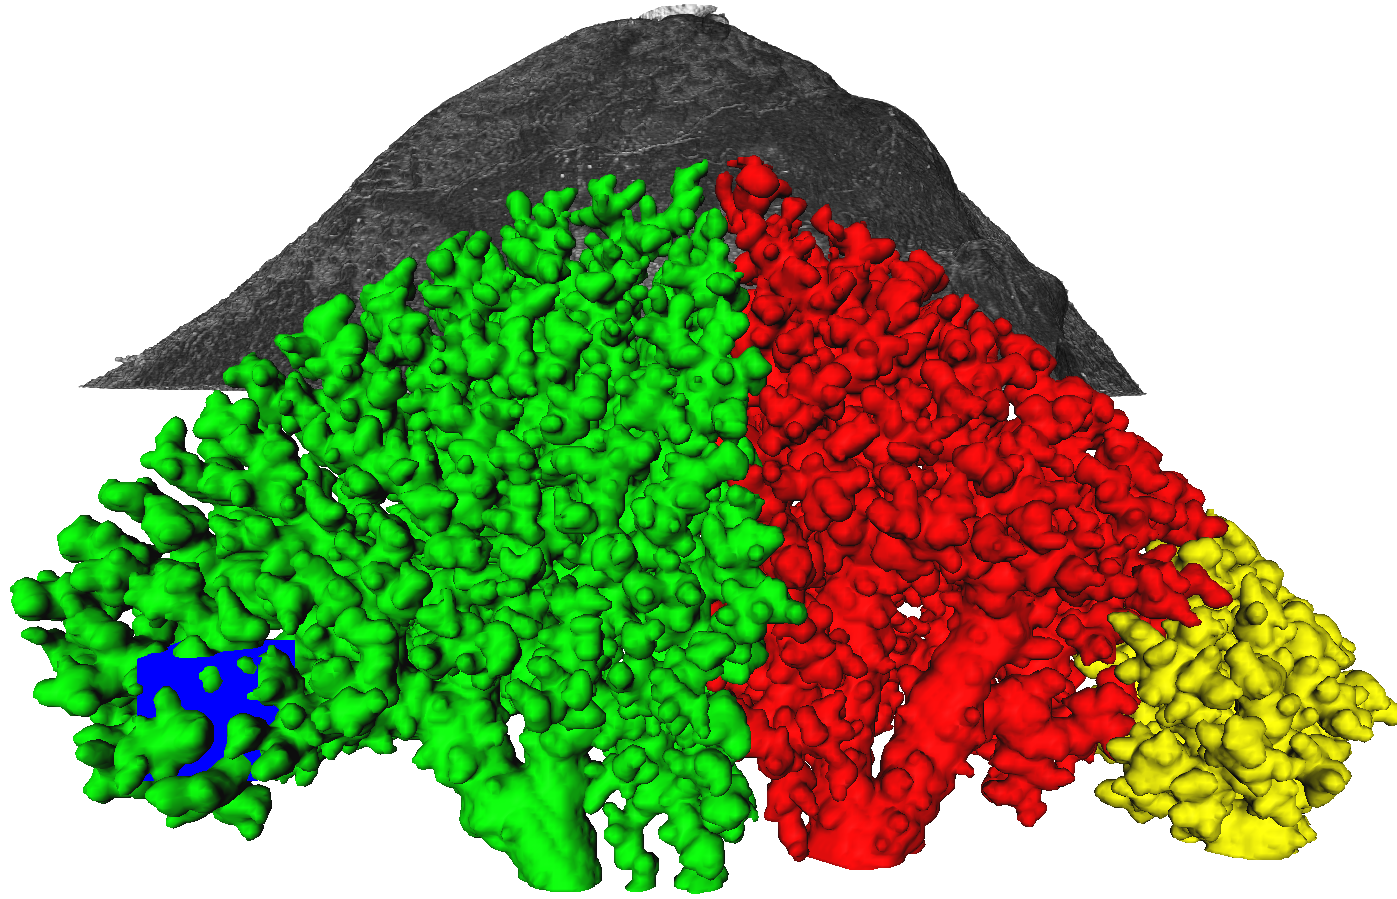
\includegraphics[width=\imagewidth]{img/comparisonBvsT/overview-b}};
%%%			% 1391px = 4.0138mm > 100px = 288um > 173px = 500um
%%%			\draw[|-|,thick] (6,774) -- (1395,839) node [sloped,midway,above] {\SI{4.0138}{\milli\meter}};
%%%			\draw[|-|,thick] (\x,\y) -- (\x+173,\y) node [midway,above] {\SI{500}{\micro\meter}};
%%%		\end{tikzpicture}%
%%%		}%
%%%	\subfloat[Overview of protocol T]{%
%%%		\label{subfig:DetailOverviewT}%
%%%		\begin{tikzpicture}[x=\imagescale,y=-\imagescale]
%%%			\node[anchor=north west,inner sep=0pt,outer sep=0pt] at (0,0)
%%%				{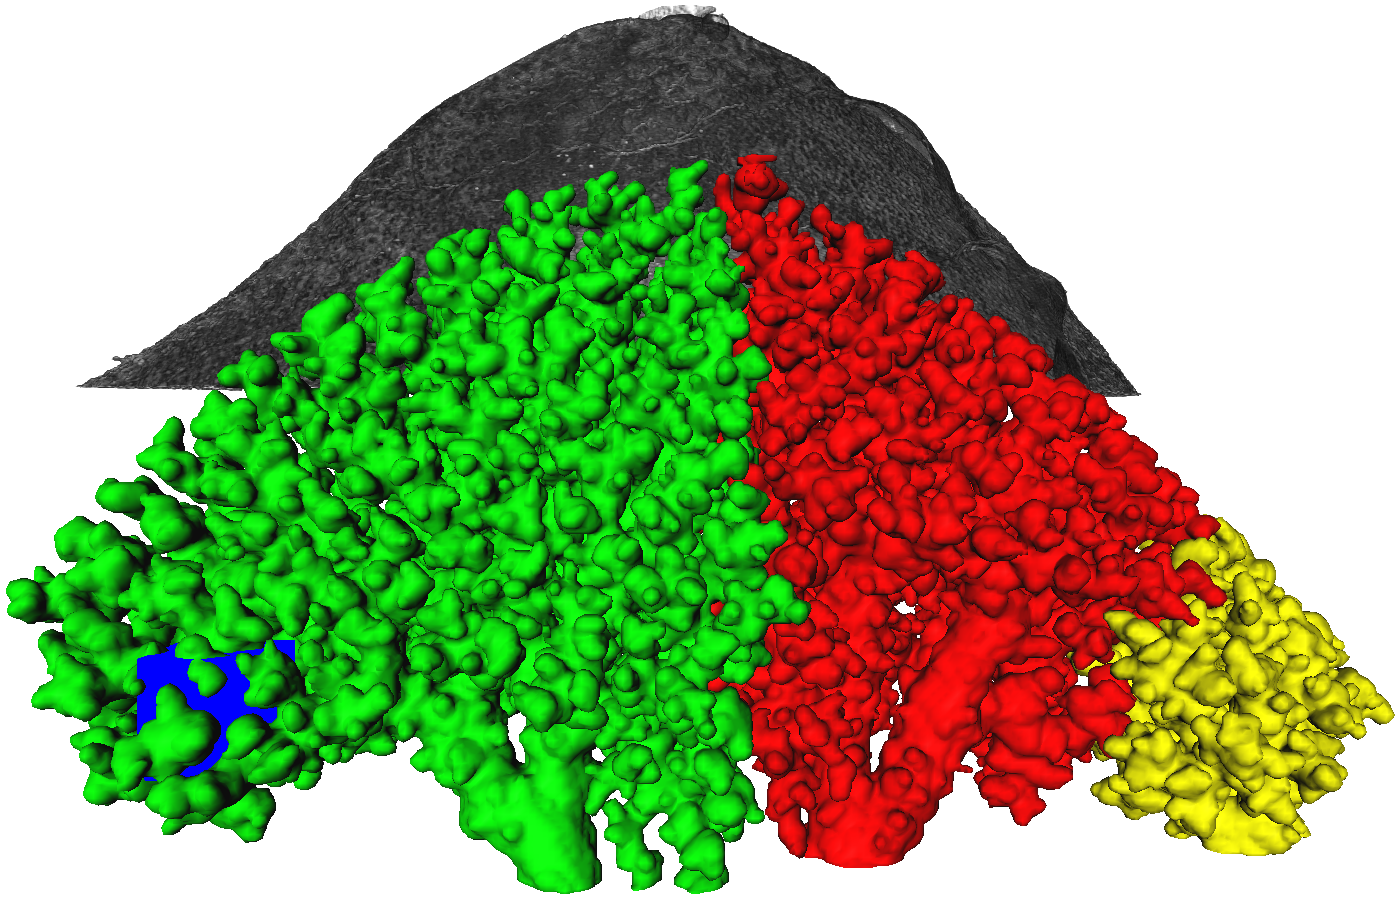
\includegraphics[width=\imagewidth]{img/comparisonBvsT/overview-t}};
%%%			% 1391px = 4.0138mm > 100px = 288um > 173px = 500um
%%%			\draw[|-|,thick] (6,774) -- (1395,839) node [sloped,midway,above] {\SI{4.0138}{\milli\meter}};
%%%			\draw[|-|,thick] (\x,\y) -- (\x+173,\y) node [midway,above] {\SI{500}{\micro\meter}};
%%%		\end{tikzpicture}%
%%%		}\\%
%%%	\pgfmathsetlength{\imagescale}{\imagewidth/806} % pixel width of imagefile used
%%%	\def\x{345}
%%%	\def\y{780}
%%%	\subfloat[ROI inside green segment for protocol B]{%
%%%		\label{subfig:DetailROIB}%
%%%		\begin{tikzpicture}[x=\imagescale,y=-\imagescale]
%%%			\node[anchor=north west,inner sep=0pt,outer sep=0pt] at (0,0)
%%%				{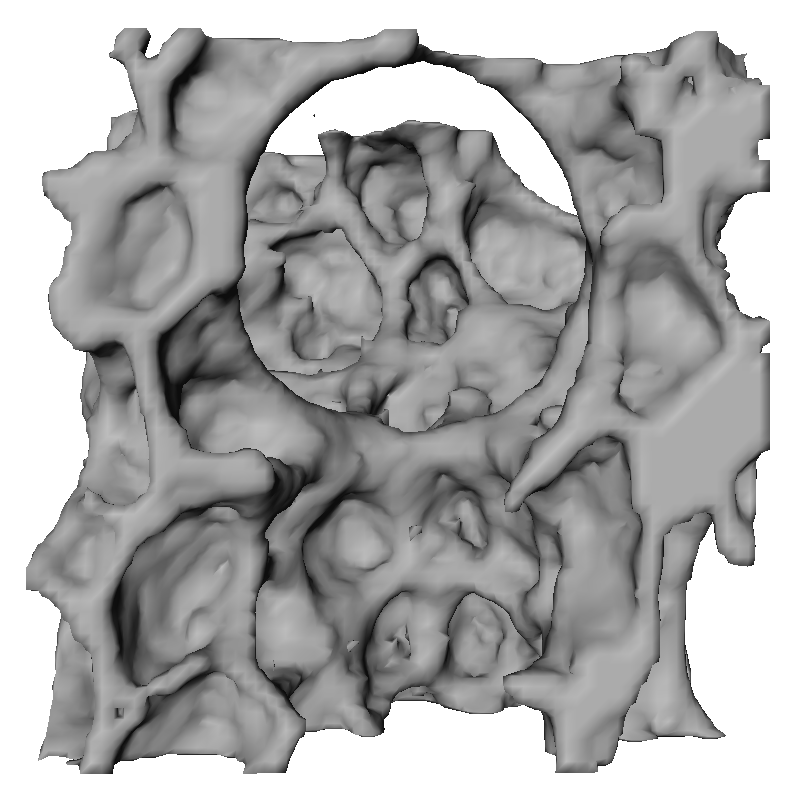
\includegraphics[width=\imagewidth]{img/comparisonBvsT/roi-b-nomedian}};
%%%			% 746px = 0.18944mm > 100px = 25um > 196.9px = 50um
%%%			\draw[|-|,thick] (27,270) -- (773,272) node [sloped,midway,above] {\SI{189.44}{\micro\meter}};
%%%			\draw[|-|,thick] (\x,\y) -- (\x+196.9,\y) node [midway,above] {\SI{50}{\micro\meter}};
%%%		\end{tikzpicture}%
%%%		}%
%%%	\subfloat[ROI inside green segment for protocol T]{%
%%%		\label{subfig:DetailROIT}%
%%%		\begin{tikzpicture}[x=\imagescale,y=-\imagescale]
%%%			\node[anchor=north west,inner sep=0pt,outer sep=0pt] at (0,0)
%%%				{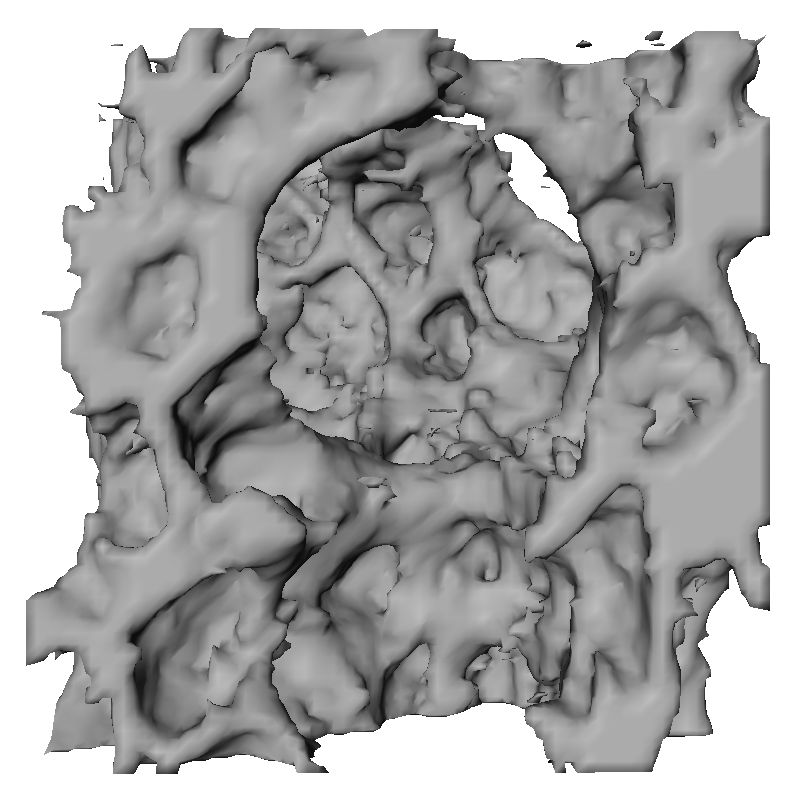
\includegraphics[width=\imagewidth]{img/comparisonBvsT/roi-t-nomedian}};
%%%			% 744px = 0.18944mm > 100px = 25um > 196.5px = 50um
%%%			\draw[|-|,thick] (27,311) -- (771,311) node [sloped,midway,above] {\SI{189.44}{\micro\meter}};
%%%			\draw[|-|,thick] (\x,\y) -- (\x+196.5,\y) node [midway,above] {\SI{50}{\micro\meter}};
%%%		\end{tikzpicture}%
%%%		}%\\%
%%%	%\subfloat[Detail B, median filtered ($3\times3\times3$)]{%
%%%	%	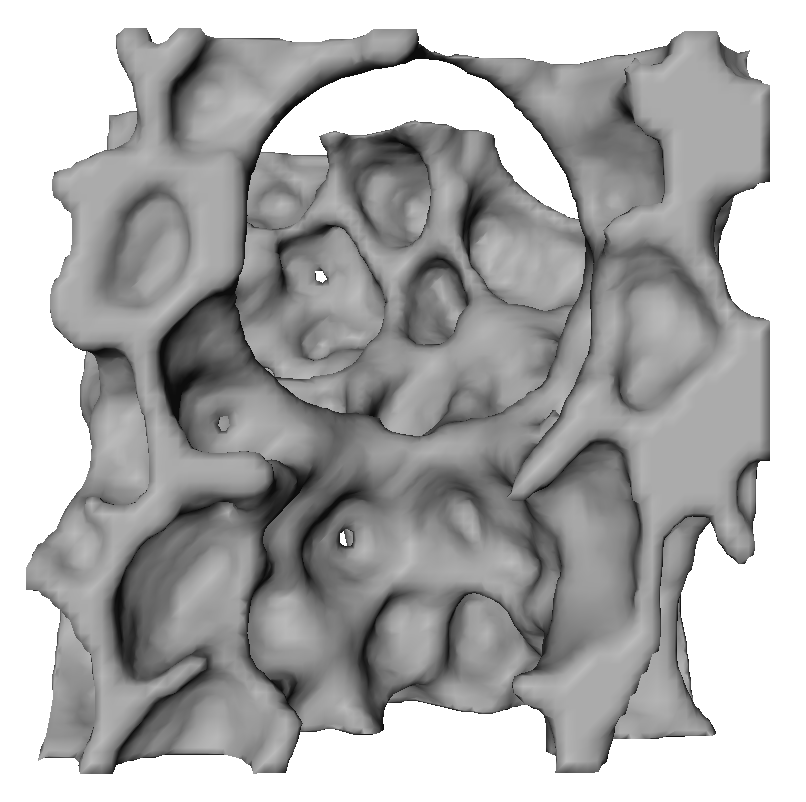
\includegraphics[width=\imsize]{img/comparisonBvsT/roi-b}%
%%%	%	}%
%%%	%\subfloat[Detail T, median filtered ($3\times3\times3$)]{%
%%%	%	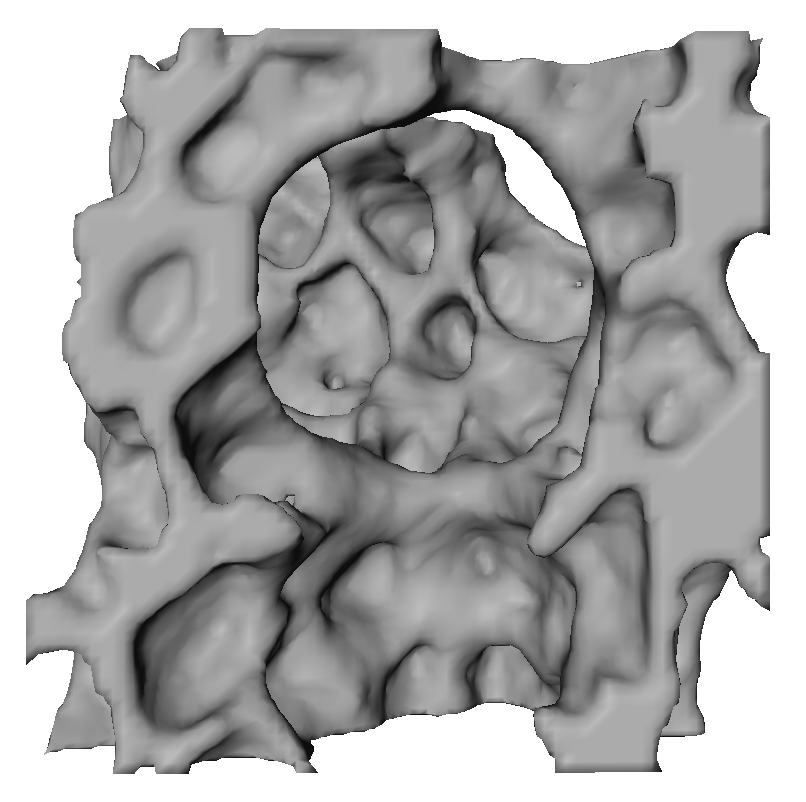
\includegraphics[width=\imsize]{img/comparisonBvsT/roi-t}%
%%%	%	}%
%%%%	\caption[Comparison of 3D visualizations of protocols B and T]
%%%	\caption{Comparison of three-dimensional visualizations of protocols B and T. Top: Three independent airway segments (green, red, yellow) have been extracted using a region growing algorithm. A cubical region of interest (ROI, blue) with a side length of 128 pixels (corresponding to \SI{190}{\micro\meter}) is marked inside the leftmost segment for both protocols. Bottom: Detailed view of isosurfaces of the lung tissue inside the ROIs shown above. Note the artifacts in the reconstructions for protocol T in subfigure~\subref{subfig:DetailROIT}.}%
%%%	\label{fig:BvsT2}%
%%%\end{figure*}
%%% normal figures %%%

As a proof of concept, we also scanned and reconstructed a lung sample with 5 subscans, which led to a roughly five-fold (4.74$\times$) increase in available FOV from 2048$\times$2048 pixels to 9703$\times$9703 pixels (see figure~\ref{fig:LungSlabSophie}). We have been able to reconstruct a sample with size of approximately 0.4$\times$3.6$\times$\SI{0.7}{\milli\meter} at a voxel side length of \SI{0.73}{\micro\meter}, see figure~\ref{fig:LungSlabSophie}.

%%% iucr %%%
%\onecolumn
\begin{figure}%
	\centering%
	\caption{Visualization of lung tissue slab:%
			a): Three dimensional volume rendering of slab of lung tissue with a size of 554$\times$4854$\times$1024 pixels at a voxel side length of \SI{0.73}{\micro\meter}. Both inset cubes have a side length of 256 pixels and were automatically segmented using a region growing algorithm. %
			b): Close-up of inset cube at an outer position in the sample, including the background tissue. % 
			c): Close-up of inset cube at an outer position in the sample. Albeit we have been able to automatically segment the lung tissue, segmentation artifacts are visible. Single alveoli can be distinguished. %
			d): Close-up of inset cube at a central position in the sample. Single alveoli are clearly visible. %
			e): Close-up of inset cube at a central position in the sample, including the background tissue.%
	 		}%
	\begin{tabular}{c}%
		\renewcommand{\imsize}{\linewidth}%
		\pgfmathsetlength{\imagewidth}{\imsize}%
		\pgfmathsetlength{\imagescale}{\imagewidth/1589}%
		\begin{tikzpicture}[x=\imagescale,y=-\imagescale]%
			\def\x{982}% scalebar-x at golden ratio
			\def\y{655}% scalebar-y at 90% of height
			\node[anchor=north west,inner sep=0pt,outer sep=0pt] at (0,0)%
				{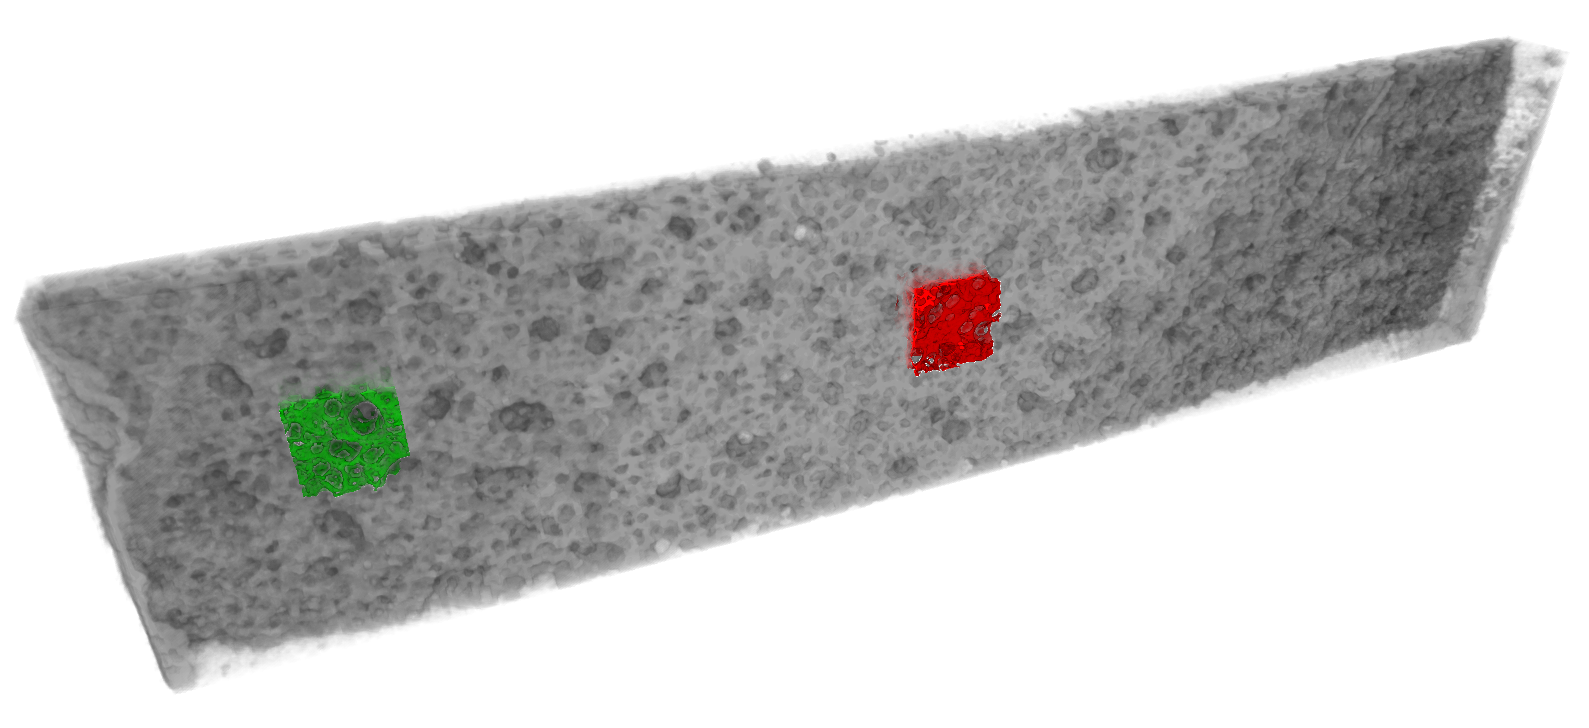
\includegraphics[width=\imagewidth]{img/sophie/full.png}};%
			% 1572px = 3.592mm > 100px = 228um > 219px = 500um
			\draw[|-|,thick] (17,319) -- (1568,58) node [sloped,midway,above] {\SI{3.592}{\milli\meter}};%
			\draw[|-|,thick] (\x,\y) -- (\x+219,\y) node [midway,above] {\SI{500}{\micro\meter}};%
		\end{tikzpicture}%
	\\%
	a) Volume Rendering of lung tissue slab, including two ROIs.%
	\\%
	\label{subfig:LungSlab}%
	\end{tabular}\\%
	\begin{tabular}{cccc}%
			\renewcommand{\imsize}{.21\linewidth}%
			\pgfmathsetlength{\imagewidth}{\imsize}% desired displayed width of image
			\pgfmathsetlength{\imagescale}{\imagewidth/902}% 1543*928 = width of imagefile used below
			\def\x{557}%
			\def\y{812}%
				\begin{tikzpicture}[x=\imagescale,y=-\imagescale]%
					\node[anchor=north west,inner sep=0pt,outer sep=0pt] at (0,0)%
						{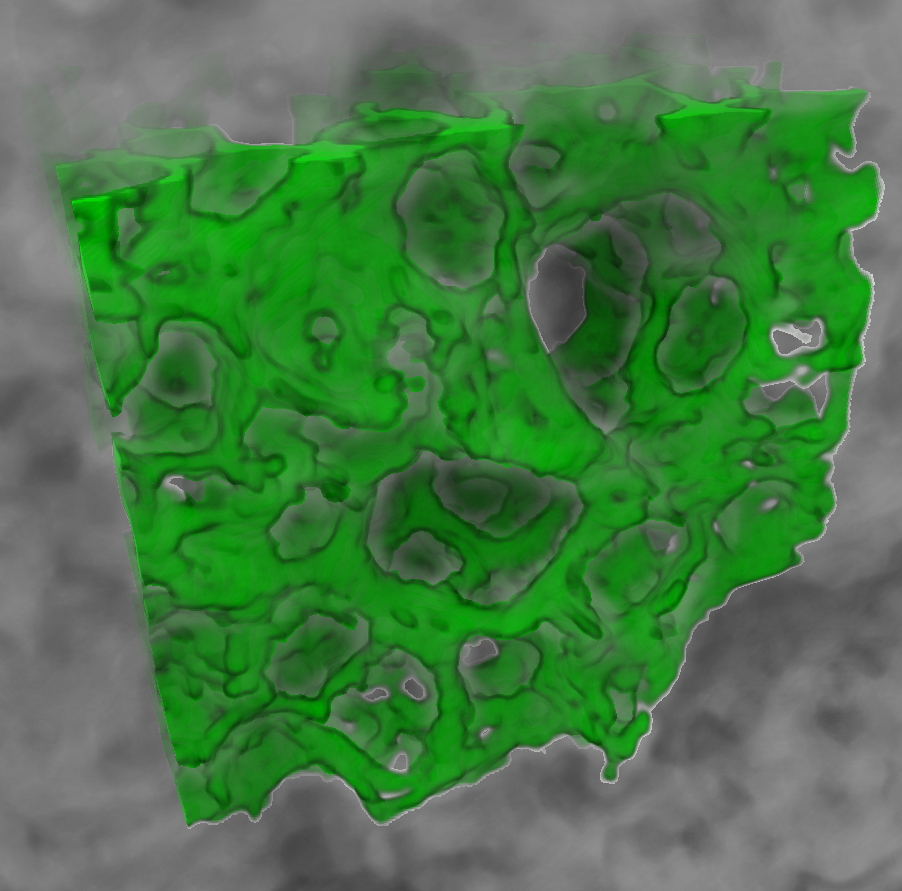
\includegraphics[width=\imagewidth]{img/sophie/crop-green-background}};%
					% 801px = 0.18944mm > 100px = 24um > 211.4px = 50um
					\draw[|-|,thick] (73,208) -- (866,93) node [sloped,midway,above] {\SI{0.18944}{\milli\meter}};%
					\draw[|-|,thick] (\x,\y) -- (\x+211.4,\y) node [midway,above] {\SI{50}{\micro\meter}};%
				\end{tikzpicture}%
				\label{subfig:LungSlabDetailsGreenBG}%
		&%
			\renewcommand{\imsize}{.21\linewidth}%
			\pgfmathsetlength{\imagewidth}{\imsize}% desired displayed width of image
			\pgfmathsetlength{\imagescale}{\imagewidth/902}% 1543*928 = width of imagefile used below
			\def\x{557}%
			\def\y{812}%
			\begin{tikzpicture}[x=\imagescale,y=-\imagescale]
				\node[anchor=north west,inner sep=0pt,outer sep=0pt] at (0,0)%
					{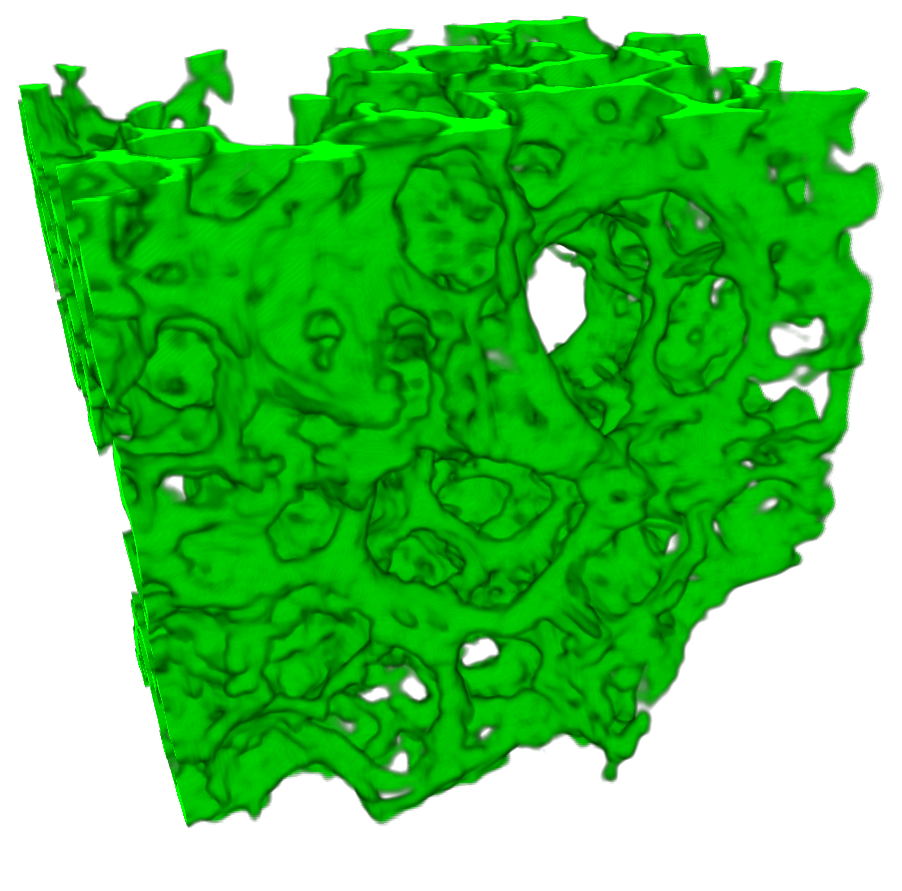
\includegraphics[width=\imagewidth]{img/sophie/crop-green}};%
				% 801px = 0.18944mm > 100px = 24um > 211.4px = 50um
				\draw[|-|,thick] (73,208) -- (866,93) node [sloped,midway,above] {\SI{0.18944}{\milli\meter}};%
				\draw[|-|,thick] (\x,\y) -- (\x+211.4,\y) node [midway,above] {\SI{50}{\micro\meter}};%
			\end{tikzpicture}%
			\label{subfig:LungSlabDetailsGreen}%
		&%
			\renewcommand{\imsize}{.21\linewidth}%
			\pgfmathsetlength{\imagewidth}{\imsize}% desired displayed width of image
			\pgfmathsetlength{\imagescale}{\imagewidth/902}% 1543*928 = width of imagefile used below
			\def\x{557}%
			\def\y{812}%
			\begin{tikzpicture}[x=\imagescale,y=-\imagescale]%
			     \node[anchor=north west,inner sep=0pt,outer sep=0pt] at (0,0)%
			         {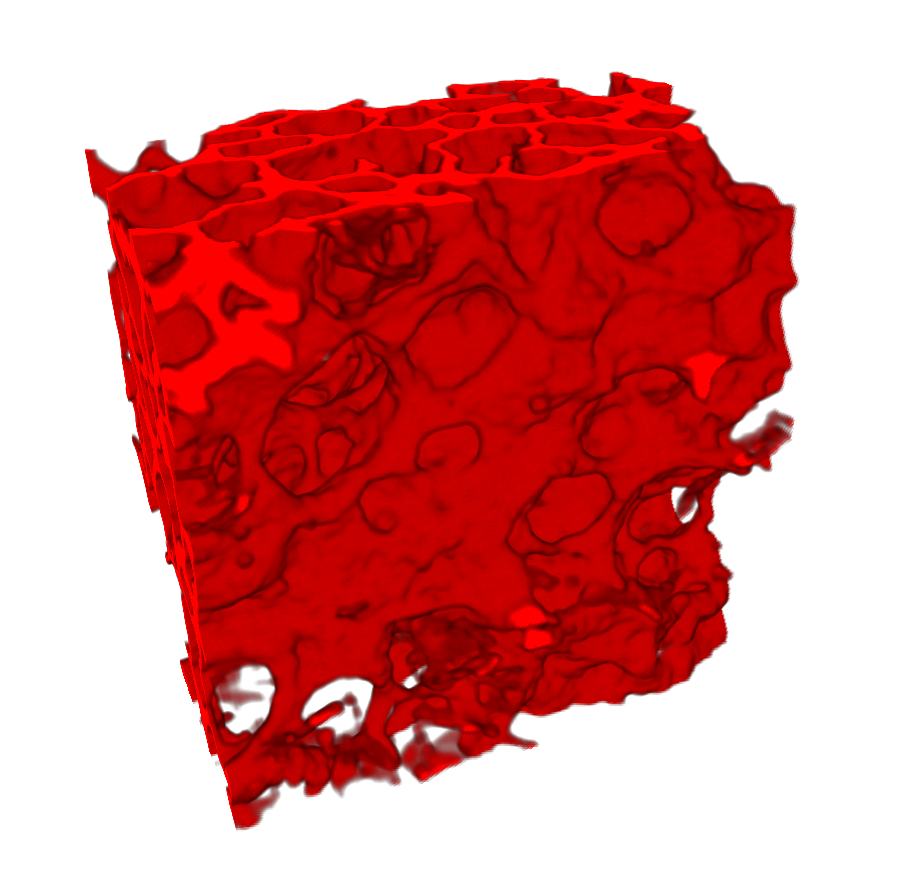
\includegraphics[width=\imagewidth]{img/sophie/crop-red}};%
				% 661px = 0.18944mm > 100px = 29um > 174.6px = 50um
				\draw[|-|,thick] (85,151) -- (741,66) node [sloped,midway,above] {\SI{189.44}{\micro\meter}};%
				\draw[|-|,thick] (\x,\y) -- (\x+174.6,\y) node [midway,above] {\SI{50}{\micro\meter}};%
			\end{tikzpicture}%
		&%
			\renewcommand{\imsize}{.21\linewidth}%
			\pgfmathsetlength{\imagewidth}{\imsize}% desired displayed width of image
			\pgfmathsetlength{\imagescale}{\imagewidth/902}% 1543*928 = width of imagefile used below
			\def\x{557}%
			\def\y{812}%
			\begin{tikzpicture}[x=\imagescale,y=-\imagescale]%
			     \node[anchor=north west,inner sep=0pt,outer sep=0pt] at (0,0)%
			         {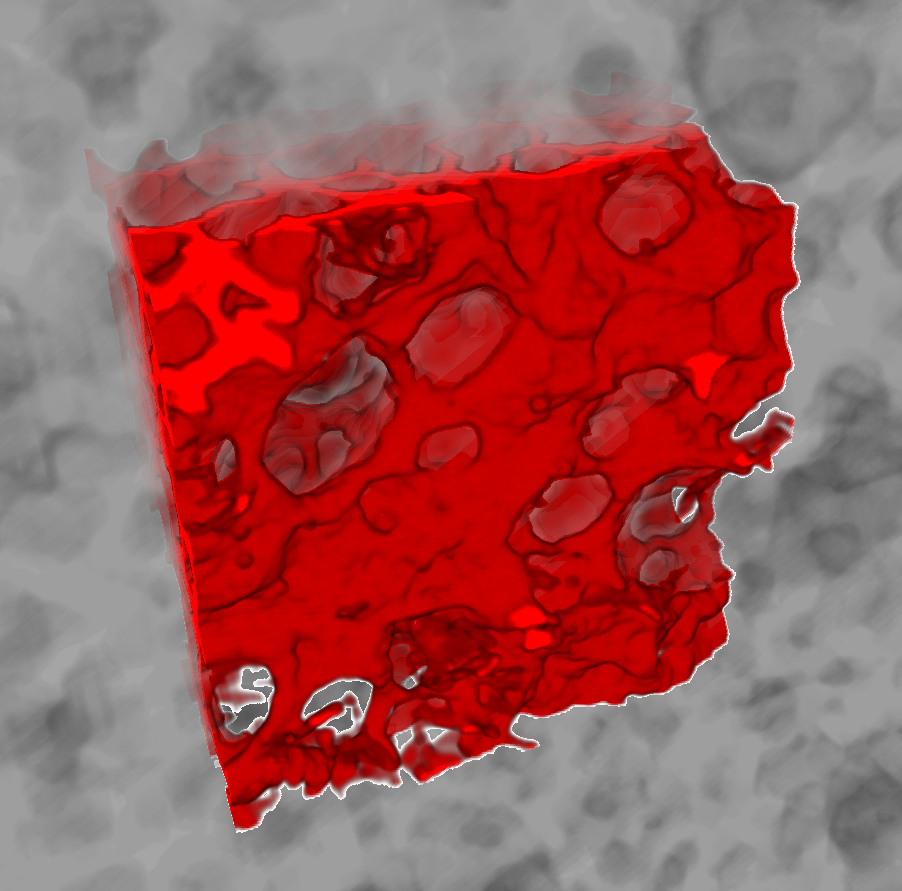
\includegraphics[width=\imagewidth]{img/sophie/crop-red-background}};%
				% 661px = 0.18944mm > 100px = 29um > 174.6px = 50um
				\draw[|-|,thick] (85,151) -- (741,66) node [sloped,midway,above] {\SI{189.44}{\micro\meter}};%
				\draw[|-|,thick] (\x,\y) -- (\x+174.6,\y) node [midway,above] {\SI{50}{\micro\meter}};%
			\end{tikzpicture}%
		 	\label{subfig:LungSlabDetailsRedBG}%
		\\%
			b) ROI inside lung tissue slab%
		&%
			c) extracted ROI%
		&%
			d) extracted ROI%
		&%
			e) ROI inside lung tissue slab%
		\\%
	\end{tabular}%
	\label{fig:LungSlabSophie}%
\end{figure}%
%\twocolumn
%%% iucr %%%
%%% normal figures %%%
%%\begin{figure*}[htp]
%%	\renewcommand{\imsize}{\linewidth}%
%%	\pgfmathsetlength{\imagewidth}{\imsize} 		 % desired displayed width of image
%%	\pgfmathsetlength{\imagescale}{\imagewidth/1589} % 1589*728 = width of imagefile used below
%%	\centering
%%	\subfloat[Volume Rendering of lung tissue slab, including two ROI]{%
%%		\begin{tikzpicture}[x=\imagescale,y=-\imagescale]
%%			\def\x{982} % scalebar-x at golden ratio
%%			\def\y{655} % scalebar-y at 90% of height
%%			\node[anchor=north west,inner sep=0pt,outer sep=0pt] at (0,0)
%%				{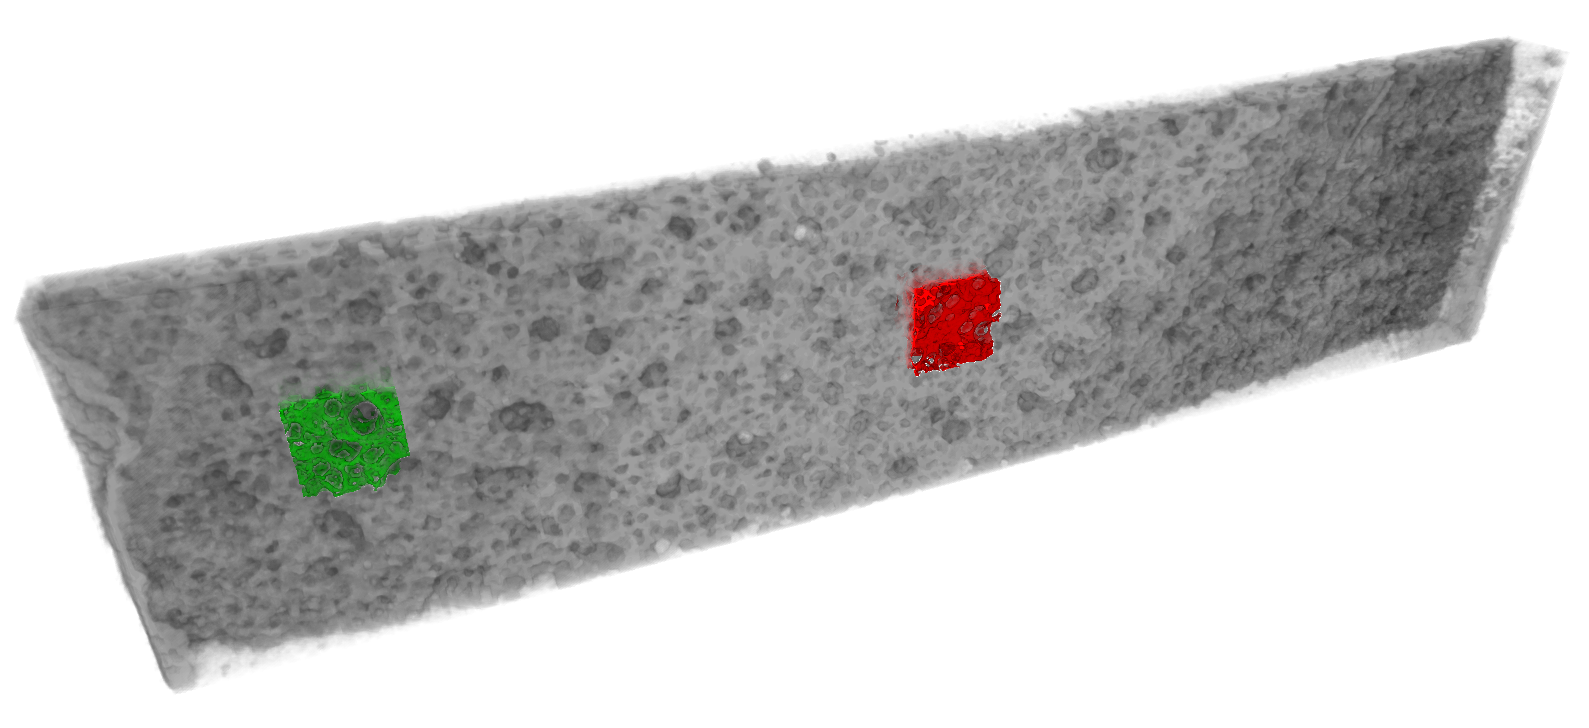
\includegraphics[width=\imagewidth]{img/sophie/full.png}};
%%			% 1572px = 3.592mm > 100px = 228um > 219px = 500um
%%			\draw[|-|,thick] (17,319) -- (1568,58) node [sloped,midway,above] {\SI{3.592}{\milli\meter}};
%%			\draw[|-|,thick] (\x,\y) -- (\x+219,\y) node [midway,above] {\SI{500}{\micro\meter}};
%%		\end{tikzpicture}%
%%		\label{subfig:LungSlab}%
%%		}%
%%	\renewcommand{\imsize}{.25\linewidth}
%%	\pgfmathsetlength{\imagewidth}{\imsize} % desired displayed width of image
%%	\pgfmathsetlength{\imagescale}{\imagewidth/902} % 1543*928 = width of imagefile used below
%%	\def\x{557}
%%	\def\y{812}
%%	\subfloat[ROI inside the lung tissue slab]{%
%%		\begin{tikzpicture}[x=\imagescale,y=-\imagescale]
%%			\node[anchor=north west,inner sep=0pt,outer sep=0pt] at (0,0)
%%				{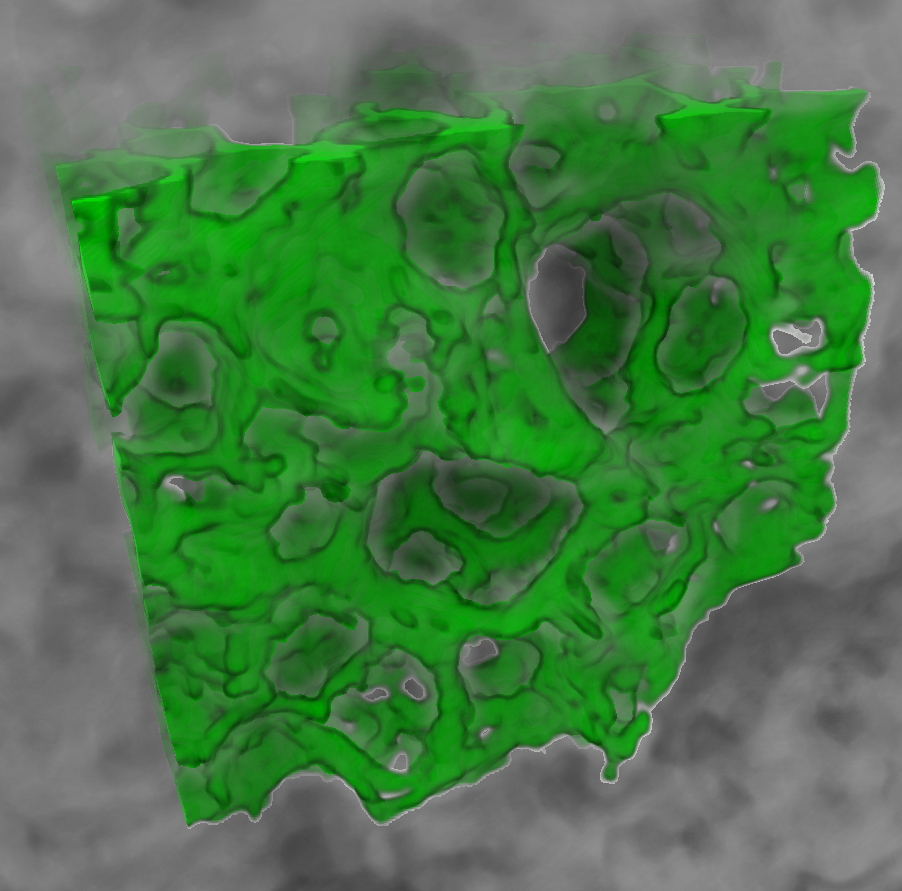
\includegraphics[width=\imagewidth]{img/sophie/crop-green-background}};
%%			% 801px = 0.18944mm > 100px = 24um > 211.4px = 50um
%%			\draw[|-|,thick] (73,208) -- (866,93) node [sloped,midway,above] {\SI{0.18944}{\milli\meter}};
%%			\draw[|-|,thick] (\x,\y) -- (\x+211.4,\y) node [midway,above] {\SI{50}{\micro\meter}};
%%		\end{tikzpicture}%
%%		\label{subfig:LungSlabDetailsGreenBG}%
%%		}%
%%	\subfloat[extracted ROI]{%
%%		\begin{tikzpicture}[x=\imagescale,y=-\imagescale]
%%			\node[anchor=north west,inner sep=0pt,outer sep=0pt] at (0,0)
%%				{\includegraphics[width=\imagewidth]{img/sophie/crop-green}};
%%			% 801px = 0.18944mm > 100px = 24um > 211.4px = 50um
%%			\draw[|-|,thick] (73,208) -- (866,93) node [sloped,midway,above] {\SI{0.18944}{\milli\meter}};
%%			\draw[|-|,thick] (\x,\y) -- (\x+211.4,\y) node [midway,above] {\SI{50}{\micro\meter}};
%%		\end{tikzpicture}%
%%	 	\label{subfig:LungSlabDetailsGreen}%
%%		}%
%%	\subfloat[ROI inside the lung tissue slab]{%
%%		\begin{tikzpicture}[x=\imagescale,y=-\imagescale]
%%		     \node[anchor=north west,inner sep=0pt,outer sep=0pt] at (0,0)
%%		         {\includegraphics[width=\imagewidth]{img/sophie/crop-red}};
%%			% 661px = 0.18944mm > 100px = 29um > 174.6px = 50um
%%			\draw[|-|,thick] (85,151) -- (741,66) node [sloped,midway,above] {\SI{189.44}{\micro\meter}};
%%			\draw[|-|,thick] (\x,\y) -- (\x+174.6,\y) node [midway,above] {\SI{50}{\micro\meter}};
%%		\end{tikzpicture}%
%%		\label{subfig:LungSlabDetailsRed}%
%%		}%
%%	\subfloat[extracted ROI]{%
%%		\begin{tikzpicture}[x=\imagescale,y=-\imagescale]
%%		     \node[anchor=north west,inner sep=0pt,outer sep=0pt] at (0,0)
%%		         {\includegraphics[width=\imagewidth]{img/sophie/crop-red-background}};
%%			% 661px = 0.18944mm > 100px = 29um > 174.6px = 50um
%%			\draw[|-|,thick] (85,151) -- (741,66) node [sloped,midway,above] {\SI{189.44}{\micro\meter}};
%%			\draw[|-|,thick] (\x,\y) -- (\x+174.6,\y) node [midway,above] {\SI{50}{\micro\meter}};
%%		\end{tikzpicture}%
%%	 	\label{subfig:LungSlabDetailsRedBG}%
%%		}%
%%%	\caption[Visualization of lung tissue slab.]
%%	\caption{Visualization of lung tissue slab: %
%%		\subref{subfig:LungSlab}: Three dimensional volume rendering of slab of lung tissue with a size of 554$\times$4854$\times$1024 pixels at a voxel side length of \SI{0.73}{\micro\meter}. Both inset cubes have a side length of 256 pixels and were automatically segmented using a region growing algorithm. 
%% 		\subref{subfig:LungSlabDetailsGreenBG}: Close-up of inset cube at an outer position in the sample, including the background tissue. % 
%% 		\subref{subfig:LungSlabDetailsGreen}: Close-up of inset cube at an outer position in the sample. Albeit we have been able to automatically segment the lung tissue, segmentation artifacts are visible. Single alveoli can be distinguished. %
%% 		\subref{subfig:LungSlabDetailsRed}: Close-up of inset cube at a central position in the sample. Single alveoli are clearly visible. %
%% 		\subref{subfig:LungSlabDetailsRedBG}: Close-up of inset cube at a central position in the sample, including the background tissue.%
%% 		}%
%%	\label{fig:LungSlabSophie}%
%%\end{figure*}
%%% normal figures %%%
%!TEX root = widefieldscan.tex
\svnidlong
{$HeadURL$}
{$LastChangedDate$}
{$LastChangedRevision$}
{$LastChangedBy$}
%
%\ifhtml
%\else
%\begin{center}
%	\fbox{
%		\begin{minipage}{.618\columnwidth}
%		The section below is versioned at \url{\svnkw{HeadURL}} (last commit @ \svnfileday.\svnfilemonth.\svnfileyear \space \svnfilehour:\svnfileminute, Revision: \svnkw{LastChangedRevision}).
%		\end{minipage}
%	} 
%\end{center}
%\fi
%
\section{Discussion}\label{sec:Discussion}%

We present a method to laterally increase the field of view of tomographic imaging systems operated in parallel beam geometry and would like to call this method wide field synchrotron radiation based x-ray tomographic microscopy (WF-SRXTM). We selectively defined different scanning protocols for the optimization of the total imaging time towards the expected imaging quality. This enables a very fast acquisition of lower quality tomographic datasets or acquisition of very high quality datasets in a longer time.

The field of view was increased three-fold by merging projections from three subscans and reconstructing the merged projections using the standard workflow present at the TOMCAT beamline. As a consequence of increasing the field of view, an increased amount of projections has to be acquired to satisfy the sampling theorem. This increased amount of projections lengthens the acquisition time. To overcome this limitation, we defined multiple scanning protocols with a reduced amount of total projections and thus reduced acquisition time. All these protocols have been evaluated for quality of the resulting reconstructions compared to a gold standard. We have shown that the resulting quality can be simulated prior to scanning, thus giving the end-user a possibility to chose a suited scanning protocol, based on the demands for scanning time optimization and quality of the resulting tomographic dataset.

For protocols with an equal amount of total projections, but differing amount of projections for the central and the ring scans we observed a difference in reconstruction quality (protocols C and D as well as protocols M and N are such protocols and are marked in figure~\ref{fig:NormalizedErrorPlot}). This difference arises through the fact that the amount of projections acquired for the central and the subscan do add up to the same total amount of projections, but contribute differently to the quality of the reconstruction. Two factors are responsible for this result: First, we perform an oversampling in the central scan for both protocols D and N when compared to protocols C and M, which increases the quality of the reconstructions. Second, since we acquired different amount of projections for the subscans, we need to interpolate projections from the central scan to generate merged projections, which accounts for an additional error for protocols M and C\todo{Additionally a ``missing wedge''-problem for outer scans?}.

It is thus desirable to favor a protocol with equal amounts of projections for each subscans over of a protocol with an equal total amount of projections, but a decreased amount of projections for the central scan. Since a reduced amount of projections for the central scan decreases the reconstruction quality for the central parts of the sample, this explanation seems natural. In addition, the interpolation of missing projections could introduce artifacts in the reconstruction which are suppressed when simply stitching projections without interpolation.

We have shown that the field of view of parallel beam tomographic end-stations can be increased up to five-fold and have three-dimensionally reconstructed multiple tomograms obtained with WF-SRXTM. The protocols are theoretically expandable for more than the shown 5 subscans, albeit the reconstruction of wide field scans with 7 or more subscans implies tremendous requirements on the data processing infrastructure. The datasets shown in figure~\ref{fig:BvsT} are binned scans resulting in datasets of 1024 slices, each with a size of 2792$\times$2792 pixels at a \SI{8}{\bit} depth. This amounts to a total size of the dataset of approximately \SI{7.5}{\giga\byte}. If we assume an un-binned scan with 7 overlapping subscans, the size of the stitched projections will be around 14000$\times$14000 pixels. The full dataset will consist of 2048 stitched slices with that size, with amounts to a total size of approximately \SI{383}{\giga\byte} for the full dataset. All mentioned datasets have been reconstructed at \SI{8}{\bit}, TOMCAT also offers the possibility to obtain tomographic datasets with \SI{16}{\bit} depth. A wide field scan with a seven-fold increase in field of view with increased bit depth would result in one dataset with a size of \SI{0.75}{\tera\byte}.

Nonetheless it is interesting to scan samples with a five-fold increase in field of view or bigger, since it would enable the end-user to selectively reconstruct regions of interest from large samples with ultra-high resolution. Up to now a two-step process was required to scan such regions from samples larger than the field of view at high resolutions. In a first step, a registered overview scan of the sample at lower resolution and thus large field of view was acquired, then a region of interest to be scanned with high resolution was marked in the low-resolution dataset using a custom-made ROI picker software~\cite{Heinzer2008} and a high resolution local tomography scan with small field of view was performed at the marked region.

One disadvantage of WF-SRXTM compared to the ROI picker method is the extremely big datasets which resulting from the reconstruction of the full resolution projections into reconstructions spanning a large field of view. With the ROI picker method only selective regions of interest selected from a low-resolution tomogram are scanned and reconstructed in high resolution, thus reducing the amount of data recorded. Since we record all data in a one-step process, it would be possible to integrate partial reconstructions of the full size datasets into the data processing pipeline of TOMCAT. After definition of a ROI to be reconstructed out of the high-resolution wide field dataset, partial sinograms and partial reconstructions could be calculated.
%!TEX root = widefieldscan.tex
\svnidlong
{$HeadURL$}
{$LastChangedDate$}
{$LastChangedRevision$}
{$LastChangedBy$}

\begin{center}
	\fbox{
		\begin{minipage}{.618\columnwidth}
		The section below is versioned at \url{\svnkw{HeadURL}} (last commit @ \svnfileday.\svnfilemonth.\svnfileyear \space \svnfilehour:\svnfileminute \space (UTC\svnfiletimezone), Revision: \svnkw{LastChangedRevision}).
		\end{minipage}
	} 
\end{center}

\section{Summary}
The proposed method establishes an increase of the visible FOV up to five times what is conventionally available. We have shown that we can provide different scanning protocols based on needs of the end-user of TOMCAT. The end-user has the possibility to choose a suitable scanning protocol depending on a balance between acquisition time and reconstruction quality. We managed to reduce the image acquisition time down to \SI{14}{\percent} of the comparable gold standard scan while keeping the quality of the reconstructed tomographic dataset on a level that still permitted automated segmentation of the lung structure and surrounding airspace, as shown in figure~\ref{fig:BvsT}.

Further increases of the FOV are only theoretically limited, but face problems with the amount of data to process. The dataset shown in figure~\ref{fig:LungSlabSophie} is composed of 1024 tiff-Files each with a size of 4852$\times$4852 pixels, which adds up to a total size of nearly \SI{23}{\giga B}. Calculations and visualizations of datasets of this size require great optimizations of the processing queue and automation of calculations\todo{elaborate a bit more\ldots}.

The stitching of the multiple overlapping projections has been automated using custom made MATLAB scripts and will be implemented at the beamline for end-user access. Since the stitching of the overlapping subscans is quite a time-consuming process it would be desirable to directly implement the stitching in to the present sinogram generation routines. This would also reduce the load on the file server, since at the moment, all the projection from the subscans are read from disk, merged to big projections and these big projections is then subsequently written to disk. If would be desirable to directly generate merged sinograms from the overlapping subscans to define the reconstruction parameters and then perform the merging and reconstruction on the cluster without intermediate merging step\todo{Is this planned? Or is this too far-fetched for TOMCAT-team?}.

\section{Outlook}
The wide field scanning method has been developed to enable the high-resolution tomographic imaging of entire acini, something which would not have been possible with the  ``simple'' tomographic imaging method present at TOMCAT.

In addition to the multiple scans of the same sample to assess the method, we also recorded tomographic datasets with increased FOV from distal-medial edges of right lower lung lobes of Sprague Dawley rats obtained at post-natal days 4, 10, 21, 36 and 60. With these samples we have begun to study the skeleton of the terminal airways to quantitatively differentiate the lung development at this post-natal stage\todo{add manuscript in preparation?}.

Figure~\ref{fig:skel} shows a three dimensional visualization of such a lung lobe including the extracted segments and the airway skeleton of such a segment. We are currently analyzing the skeletons of the terminal airways at different stages in lung development and plan to publish the morphological details as soon as possible.

\renewcommand{\imsize}{\linewidth}
\pgfmathsetlength{\imagewidth}{\imsize} % desired displayed width of image
\pgfmathsetlength{\imagescale}{\imagewidth/1520} % pixel width of imagefile used below
\begin{figure*}
	\centering
%		\subfloat[conventional scan]{ncludegraphics[width=\imsize]{img/widefieldscanning/R108C04C-skeleton-s2}
%			}\\
%		\subfloat[merge]{
%			\includegraphics[%angle=90,
%							width=\imsize]{img/widefieldscanning/R108C04C-skeleton-merge}%
			\begin{tikzpicture}[x=\imagescale,y=-\imagescale]
			\def\x{950}
			\def\y{725}
    			\node[anchor=north west,inner sep=0pt,outer sep=0pt] at (0,0)
    			{\includegraphics[width=\imagewidth]{img/widefieldscanning/R108C04C-skeleton-merge}};
		    	\draw[|-|,thick] (13,512) -- (705,572) node [midway,right] {\SI{3.8444}{\milli\meter}}; 
			    % 695 px = 3.844 mm > 100 px = 554 um > 90 px = 500um
				\draw[|-|,thick] (\x,\y) -- (180+\x,\y) node [midway,above] {\SI{1}{\milli\meter}}; 
			\end{tikzpicture}%							
%			}
	\caption{Three dimensional visualization of the distal-medial edge of the right lower lung lobe of a Sprague Dawley rat (same sample as in figure~\ref{fig:overview} and~\ref{fig:down}), including the airway skeletons of the extracted airways.}
	\label{fig:skel}
\end{figure*}
%!TEX root = widefieldscan.tex
\section{Acknowledgements}
asdf


\bibliographystyle{unsrtnat}
%\bibliography{../references}
\bibliography{references-wfs}

\appendix

%!TEX root = widefieldscan.tex

\appendix

\svnidlong
{$HeadURL$}
{$LastChangedDate$}
{$LastChangedRevision$}
{$LastChangedBy$}

\begin{center}
	\fbox{
		\begin{minipage}{.618\textwidth}
		The file of this section is \url{\svnkw{HeadURL}}, was last changed at: \svnfileday.\svnfilemonth.\svnfileyear \space \svnfilehour:\svnfileminute \space (UTC\svnfiletimezone) and is at revision \svnkw{LastChangedRevision}.
		\end{minipage}
	} 
\end{center}

\section{code}
the code can be downloaded/found on \url{http://www.ana.unibe.ch/~haberthuer/code/matlab}\todo{or don't we provide the code?}

\end{document}